% 若编译失败,且生成 .synctex(busy) 辅助文件,可能有两个原因:
% 1. 需要插入的图片不存在:Ctrl + F 搜索 'figure' 将这些代码注释/删除掉即可
% 2. 路径/文件名含中文或空格:更改路径/文件名即可

% --------------------- 文章宏包及相关设置 --------------------- %
% >> ------------------ 文章宏包及相关设置 ------------------ << %
% 设定文章类型与编码格式
\documentclass[UTF8]{report}		

% 本 .tex 专属的宏定义
    \def\uV{\ \mathrm{uV}}
    \def\mV{\ \mathrm{mV}}
    \def\V{\ \mathrm{V}}
    \def\kV{\ \mathrm{KV}}
    \def\KV{\ \mathrm{KV}}
    \def\MV{\ \mathrm{MV}}
    \def\uF{\ \mathrm{uF}}
    \def\nF{\ \mathrm{nF}}
    \def\pF{\ \mathrm{pF}}
    \def\uA{\ \mathrm{uA}}
    \def\mA{\ \mathrm{mA}}
    \def\A{\ \mathrm{A}}
    \def\kA{\ \mathrm{KA}}
    \def\KA{\ \mathrm{KA}}
    \def\MA{\ \mathrm{MA}}
    \def\uO{\ \mu\Omega}
    \def\mO{\ \mathrm{m}\Omega}
    \def\O{\ \Omega}
    \def\kO{\ \mathrm{K}\Omega}
    \def\KO{\ \mathrm{K}\Omega}
    \def\MO{\ \mathrm{M}\Omega}
    \def\Hz{\ \mathrm{Hz}}
    \def\kHz{\ \mathrm{kHz}}
    \def\KHz{\ \mathrm{KHz}}
    \def\mHz{\ \mathrm{MHz}}
    \def\MHz{\ \mathrm{MHz}}
    \def\Res{\,\mathrm{Res}\,}
    \def\Im{\,\mathrm{Im}\,}
    \def\Re{\,\mathrm{Re}\,}
    \def\db{\,\mathrm{dB}\,}
    \def\dB{\,\mathrm{dB}\,}

% 自定义宏定义
    \def\N{\mathbb{N}}
    \def\F{\mathbb{F}}
    \def\Z{\mathbb{Z}}
    \def\Q{\mathbb{Q}}
    \def\R{\mathbb{R}}
    \def\C{\mathbb{C}}
    \def\T{\mathbb{T}}
    \def\S{\mathbb{S}}
    %\def\A{\mathbb{A}}
    \def\I{\mathscr{I}}
    \def\d{\mathrm{d}}
    \def\p{\partial}


% 导入基本宏包
    \usepackage[UTF8]{ctex}     % 设置文档为中文语言
    \usepackage{hyperref}  % 宏包:自动生成超链接 (此宏包与标题中的数学环境冲突)
    \hypersetup{
        % 超链接颜色设置
        colorlinks=true,    % false:边框链接 ; true:彩色链接
        citecolor={blue},    % 文献引用颜色
        linkcolor={blue},   % 目录 (我们在目录处单独设置),公式,图表,脚注等内部链接颜色
        urlcolor={magenta},    % 网页 URL 链接颜色,包括 \href 中的 text
        % pdf 相关设置
        pdfauthor={丁毅},% PDF 作者
        pdftitle={Notes of Principles of Electric Circuits},% PDF 标题
        pdfproducer={LaTeX with hyperref}, % PDF 制作软件
        pdfcreator={xelatex},       % PDF 创建者
        pdfpagelayout=TwoColumn,    % 双栏布局
        pdfstartview=FitH,          % 页面宽度适合窗口
        %pdfpagemode=UseNone,       % 不显示书签 (默认会显示)
        pdfpagemode=UseOutlines,    % 显示书签
        pdfnewwindow=true,          % 在新窗口中打开链接
        pdfencoding=auto,           % 自动编码
        pdfborder={0 0 0},          % pdf 无边框
        pdfhighlight=/I,            % 链接高亮样式
        % magenta 洋红色
        % cyan 浅蓝色 
        % magenta 洋红色
        % yellow 黄色
        % black 黑色
        % white 白色
        % red 红色
        % green 绿色
        % blue 蓝色
        % gray 灰色
        % darkgray 深灰色
        % lightgray 浅灰色
        % brown 棕色
        % lime 石灰色
        % olive 橄榄色
        % orange 橙色
        % pink 粉红色
        % purple 紫色
        % teal 蓝绿色
        % violet 紫罗兰色
    }
    % \usepackage{docmute}    % 宏包:子文件导入时自动去除导言区,用于主/子文件的写作方式,\include{./51单片机笔记}即可。注:启用此宏包会导致.tex文件capacity受限。
    \usepackage{amsmath}    % 宏包:数学公式
    \usepackage{mathrsfs}   % 宏包:提供更多数学符号
    \usepackage{amssymb}    % 宏包:提供更多数学符号
    \usepackage{pifont}     % 宏包:提供了特殊符号和字体
    \usepackage{extarrows}  % 宏包:更多箭头符号 
    \usepackage{multicol}   % 宏包:支持多栏 

% 文章页面margin设置
    \usepackage[a4paper]{geometry}
        \geometry{top=0.75in}
        \geometry{bottom=0.75in}
        \geometry{left=0.75in}
        \geometry{right=0.75in}   % 设置上下左右页边距
        \geometry{marginparwidth=1.75cm}    % 设置边注距离(注释、标记等)

% 配置数学环境
    \usepackage{amsthm} % 宏包:数学环境配置
    % theorem-line 环境自定义
        \newtheoremstyle{MyLineTheoremStyle}% <name>
            {11pt}% <space above>
            {11pt}% <space below>
            {\kaishu}% <body font> 默认使用正文字体, \kaishu 为楷体
            {}% <indent amount>
            {\bfseries}% <theorem head font> 设置标题项为加粗
            {:\ \ }% <punctuation after theorem head>
            {.5em}% <space after theorem head>
            {\textbf{#1}\thmnumber{#2}\ \ (\,\textbf{#3}\,)}% 设置标题内容顺序
        \theoremstyle{MyLineTheoremStyle} % 应用自定义的定理样式
        \newtheorem{LineTheorem}{Theorem.\,}
    % theorem-block 环境自定义
        \newtheoremstyle{MyBlockTheoremStyle}% <name>
            {11pt}% <space above>
            {11pt}% <space below>
            {\kaishu}% <body font> 使用默认正文字体
            {}% <indent amount>
            {\bfseries}% <theorem head font> 设置标题项为加粗
            {:\\ \indent}% <punctuation after theorem head>
            {.5em}% <space after theorem head>
            {\textbf{#1}\thmnumber{#2}\ \ (\,\textbf{#3}\,)}% 设置标题内容顺序
        \theoremstyle{MyBlockTheoremStyle} % 应用自定义的定理样式
        \newtheorem{BlockTheorem}[LineTheorem]{Theorem.\,} % 使用 LineTheorem 的计数器
    % definition 环境自定义
        \newtheoremstyle{MySubsubsectionStyle}% <name>
            {11pt}% <space above>
            {11pt}% <space below>
            {}% <body font> 使用默认正文字体
            {}% <indent amount>
            {\bfseries}% <theorem head font> 设置标题项为加粗
            {:\\ \indent}% <punctuation after theorem head>
            {0pt}% <space after theorem head>
            {\textbf{#3}}% 设置标题内容顺序
        \theoremstyle{MySubsubsectionStyle} % 应用自定义的定理样式
        \newtheorem{definition}{}

%宏包:有色文本框(proof环境)及其设置
    \usepackage[dvipsnames,svgnames]{xcolor}    %设置插入的文本框颜色
    \usepackage[strict]{changepage}     % 提供一个 adjustwidth 环境
    \usepackage{framed}     % 实现方框效果
        \definecolor{graybox_color}{rgb}{0.95,0.95,0.96} % 文本框颜色。修改此行中的 rgb 数值即可改变方框纹颜色,具体颜色的rgb数值可以在网站https://colordrop.io/ 中获得。(截止目前的尝试还没有成功过,感觉单位不一样)(找到喜欢的颜色,点击下方的小眼睛,找到rgb值,复制修改即可)
        \newenvironment{graybox}{%
        \def\FrameCommand{%
        \hspace{1pt}%
        {\color{gray}\small \vrule width 2pt}%
        {\color{graybox_color}\vrule width 4pt}%
        \colorbox{graybox_color}%
        }%
        \MakeFramed{\advance\hsize-\width\FrameRestore}%
        \noindent\hspace{-4.55pt}% disable indenting first paragraph
        \begin{adjustwidth}{}{7pt}%
        \vspace{2pt}\vspace{2pt}%
        }
        {%
        \vspace{2pt}\end{adjustwidth}\endMakeFramed%
        }

% 外源代码插入设置
    % matlab 代码插入设置
    \usepackage{matlab-prettifier}
        \lstset{style=Matlab-editor}    % 继承 matlab 代码高亮 , 此行不能删去
    \usepackage[most]{tcolorbox} % 引入tcolorbox包 
    \usepackage{listings} % 引入listings包
        \tcbuselibrary{listings, skins, breakable}
        \newfontfamily\codefont{Consolas} % 定义需要的 codefont 字体
        \lstdefinestyle{MatlabStyle_inc}{   % 插入代码的样式
            language=Matlab,
            basicstyle=\small\ttfamily\codefont,    % ttfamily 确保等宽 
            breakatwhitespace=false,
            breaklines=true,
            captionpos=b,
            keepspaces=true,
            numbers=left,
            numbersep=15pt,
            showspaces=false,
            showstringspaces=false,
            showtabs=false,
            tabsize=2,
            xleftmargin=15pt,   % 左边距
            %frame=single, % single 为包围式单线框
            frame=shadowbox,    % shadowbox 为带阴影包围式单线框效果
            %escapeinside=``,   % 允许在代码块中使用 LaTeX 命令 (此行无用)
            %frameround=tttt,    % tttt 表示四个角都是圆角
            framextopmargin=0pt,    % 边框上边距
            framexbottommargin=0pt, % 边框下边距
            framexleftmargin=5pt,   % 边框左边距
            framexrightmargin=5pt,  % 边框右边距
            rulesepcolor=\color{red!20!green!20!blue!20}, % 阴影框颜色设置
            %backgroundcolor=\color{blue!10}, % 背景颜色
        }
        \lstdefinestyle{MatlabStyle_src}{   % 插入代码的样式
            language=Matlab,
            basicstyle=\small\ttfamily\codefont,    % ttfamily 确保等宽 
            breakatwhitespace=false,
            breaklines=true,
            captionpos=b,
            keepspaces=true,
            numbers=left,
            numbersep=15pt,
            showspaces=false,
            showstringspaces=false,
            showtabs=false,
            tabsize=2,
        }
        \newtcblisting{matlablisting}{
            %arc=2pt,        % 圆角半径
            % 调整代码在 listing 中的位置以和引入文件时的格式相同
            top=0pt,
            bottom=0pt,
            left=-5pt,
            right=-5pt,
            listing only,   % 此句不能删去
            listing style=MatlabStyle_src,
            breakable,
            colback=white,   % 选一个合适的颜色
            colframe=black!0,   % 感叹号后跟不透明度 (为 0 时完全透明)
        }
        \lstset{
            style=MatlabStyle_inc,
        }

% table 支持
    \usepackage{booktabs}   % 宏包:三线表
    \usepackage{tabularray} % 宏包:表格排版
    \usepackage{longtable}  % 宏包:长表格

% figure 设置
    \usepackage{graphicx}  % 支持 jpg, png, eps, pdf 图片 
    \usepackage{svg}       % 支持 svg 图片
        \svgsetup{
            % 指向 inkscape.exe 的路径
            inkscapeexe = C:/aa_MySame/inkscape/bin/inkscape.exe, 
            % 一定程度上修复导入后图片文字溢出几何图形的问题
            inkscapelatex = false                 
        }
    \usepackage{subcaption} % 用于子图和小图注  

% 图表进阶设置
    \usepackage{caption}    % 图注、表注
        \captionsetup[figure]{name=图}  
        \captionsetup[table]{name=表}
        \captionsetup{
            labelfont=bf, % 设置标签为粗体
            textfont=bf,  % 设置文本为粗体
            font=small  
        }
    \usepackage{float}     % 图表位置浮动设置 
    \usepackage{etoolbox} % 用于保证图注表注的数学字符为粗体
        \AtBeginEnvironment{figure}{\boldmath} % 图注中的数学字符为粗体
        \AtBeginEnvironment{table}{\boldmath}  % 表注中的数学字符为粗体
        \AtBeginEnvironment{tabular}{\unboldmath}   % 保证表格中的数学字符不受额外影响

% 圆圈序号自定义
    \newcommand*\circled[1]{\tikz[baseline=(char.base)]{\node[shape=circle,draw,inner sep=0.8pt, line width = 0.03em] (char) {\small \bfseries #1};}}   % TikZ solution

% 列表设置
    \usepackage{enumitem}   % 宏包:列表环境设置
        \setlist[enumerate]{
            label=(\arabic*) ,   % 设置序号样式为加粗的 (1) (2) (3)
            ref=\arabic*, % 如果需要引用列表项,这将决定引用格式(这里仍然使用数字)
            itemsep=0pt, parsep=0pt, topsep=0pt, partopsep=0pt, leftmargin=3.5em} 
        \setlist[itemize]{itemsep=0pt, parsep=0pt, topsep=0pt, partopsep=0pt, leftmargin=3.5em}
        \newlist{circledenum}{enumerate}{1} % 创建一个新的枚举环境  
        \setlist[circledenum,1]{  
            label=\protect\circled{\arabic*}, % 使用 \arabic* 来获取当前枚举计数器的值,并用 \circled 包装它  
            ref=\arabic*, % 如果需要引用列表项,这将决定引用格式(这里仍然使用数字)
            itemsep=0pt, parsep=0pt, topsep=0pt, partopsep=0pt, leftmargin=3.5em
        }  

% 其它设置
    % 脚注设置
        \renewcommand\thefootnote{\ding{\numexpr171+\value{footnote}}}
    % 参考文献引用设置
        \bibliographystyle{unsrt}   % 设置参考文献引用格式为unsrt
        \newcommand{\upcite}[1]{\textsuperscript{\cite{#1}}}     % 自定义上角标式引用
    % 文章序言设置
        \newcommand{\cnabstractname}{序言}
        \newenvironment{cnabstract}{%
            \par\Large
            \noindent\mbox{}\hfill{\bfseries \cnabstractname}\hfill\mbox{}\par
            \vskip 2.5ex
            }{\par\vskip 2.5ex}

% 文章默认字体设置
    \usepackage{fontspec}   % 宏包:字体设置
        \setmainfont{SimSun}    % 设置中文字体为宋体字体
        \setCJKmainfont[AutoFakeBold=3]{SimSun} % 设置加粗字体为 SimSun 族,AutoFakeBold 可以调整字体粗细
        \setmainfont{Times New Roman} % 设置英文字体为Times New Roman

% 各级标题自定义设置
    \usepackage{titlesec}   
        % chapter 标题自定义设置
        \titleformat{\chapter}[hang]{\normalfont\huge\bfseries\centering\boldmath}{第\,\thechapter\,章}{20pt}{}
        \titlespacing*{\chapter}{0pt}{-20pt}{20pt} % 控制上下间距
        % section标题自定义设置 
        \titleformat{\section}[hang]{\normalfont\Large\bfseries\boldmath}{§\,\thesection\,}{8pt}{}
        % subsubsection标题自定义设置
        \titlespacing*{\subsubsection}{0pt}{3pt}{0pt} % 控制上下间距


% --------------------- 文章宏包及相关设置 --------------------- %
% >> ------------------ 文章宏包及相关设置 ------------------ << %

% ------------------------ 文章信息区 ------------------------ %
% ------------------------ 文章信息区 ------------------------ %
% 页眉页脚设置
    \usepackage{fancyhdr}   % 宏包:页眉页脚设置
        \pagestyle{fancy}
        \fancyhf{}
        \cfoot{\thepage}
        \renewcommand\headrulewidth{1pt}
        \renewcommand\footrulewidth{0pt}
        \usepackage{fontawesome}    % 宏包:更多符号与图标 (用于插入 GitHub 图标等)
        \lhead{\small
        \href{https://github.com/YiDingg/LatexNotes}{\color{black}\faGithub\ https://github.com/YiDingg/LatexNotes}
        }
        \chead{Notes of Principles of Electric Circuits}    
        \rhead{\small dingyi233@mails.ucas.ac.cn}

%文档信息设置
    \title{电路原理笔记\\ Notes of Principles of Electric Circuits}
    \author{丁毅\\ \footnotesize 中国科学院大学,北京 100049\\ Yi Ding \\ \footnotesize University of Chinese Academy of Sciences, Beijing 100049, China}
    \date{\footnotesize 2024.8 -- 2025.1}
% ------------------------ 文章信息区 ------------------------ %
% ------------------------ 文章信息区 ------------------------ %

% 开始编辑文章

\begin{document} 
\zihao{5}           % 设置全文字号大小

% ------------------------ 封面序言与目录 ------------------------ %
% >> --------------------- 封面序言与目录 --------------------- << %
% 封面
    \maketitle\newpage  
    \pagenumbering{Roman} % 页码为大写罗马数字
    \thispagestyle{fancy}   % 显示页码、页眉等

% 序言
\begin{cnabstract}\normalsize 
本文为笔者本科时的“电路原理”课程笔记(Notes of Principles of Electric Circuits, 2024.8 - 2025.1)。读者可到网址 \href{https://www.123865.com/s/0y0pTd-L8Kj3}{https://www.123865.com/s/0y0pTd-L8Kj3} 下载相关资料,也可以在笔者的个人网站上找到课程信息、作业答案等资料: 
\href{https://yidingg.github.io/YiDingg/\#/Notes/MajorCourses/CircuitTheoryNotes}{https://yidingg.github.io/YiDingg/\#/Notes/MajorCourses/CircuitTheoryNotes}。

由于个人学识浅陋,认识有限,文中难免有不妥甚至错误之处,望读者不吝指正。读者可以将错误发送到我的邮箱 {\color{blue}\ dingyi233@mails.ucas.ac.cn},也可以到笔者的 \href{https://github.com/YiDingg/LatexNotes}{GitHub (https://github.com/YiDingg/LatexNotes)} 上提 issue,衷心感谢。

\end{cnabstract}
\addcontentsline{toc}{chapter}{序言} % 手动添加为目录

% 目录
    \setcounter{tocdepth}{2}    % 目录深度 (为 1 时显示到 section)
    % 目录页
        \tableofcontents
        \addcontentsline{toc}{chapter}{目录}
        \thispagestyle{fancy}                   % 显示页码、页眉等
    % 插图页
        %\cleardoublepage\listoffigures
        %\addcontentsline{toc}{chapter}{插图}
        %\thispagestyle{fancy}                   % 显示页码、页眉等
    % 表格页
        %\cleardoublepage\listoftables
        %\addcontentsline{toc}{chapter}{表格}
        %\thispagestyle{fancy}                   % 显示页码、页眉等 

% 收尾工作
    \newpage    
    \pagenumbering{arabic} 


% >> --------------------- 封面序言与目录 --------------------- << %
% ------------------------ 封面序言与目录 ------------------------ %

\chapter{绪论}\thispagestyle{fancy}

本章首先介绍几个有关电路的基本问题,然后介绍电路中相关物理量的定义,再简单介绍电路在信号处理与能量处理方面的应用,最后讨论电路的分类。本章是所有后续章节的共同基础。

\section{电路}
一般来讲,电路的研究内容分为电路分析、电路综合,分别对应电路研究的正问题(已知电路求电路的解)和逆问题(已知解求电路结构参数),本课程的重点在电路分析,对电路综合不深入探讨。

有些电路原理课程习惯用大写英文字母表示不随时间变化的常量,用小写英文字母表示随时间变化的量。在本笔记中,时变量(非恒定量)、瞬时量、微元量均用小写表示,其它情况一般用大写。

\begin{figure}[H]\centering
\begin{subfigure}[t]{0.52\textwidth}\centering
    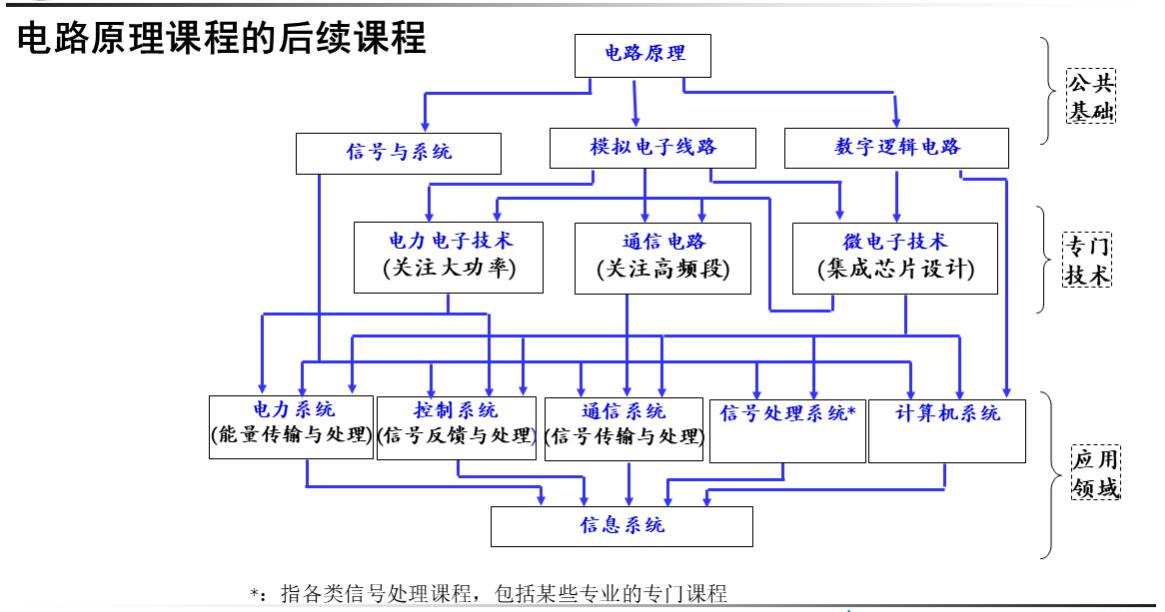
\includegraphics[height=130pt]{assets/1,2/11b7879b24f71ddbf3e5316424203201.jpg}
    \caption{ 电路原理与其他电类主要课程的联系 }
\end{subfigure}\begin{subfigure}[t]{0.48\textwidth}\centering
    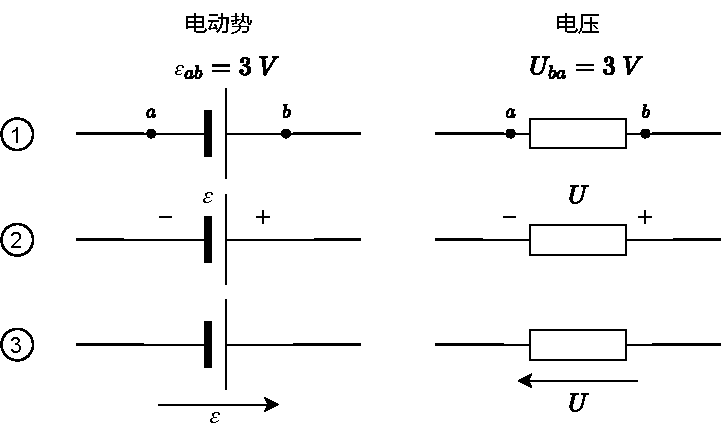
\includegraphics[height=130pt]{assets/1,2/电动势与电压.drawio.pdf}
    \caption{ 电压与电动势的三种表示方法 }
\end{subfigure}
\caption{ 电路原理与其他电类主要课程的联系、电压与电动势的三种表示方法 }\label{电路原理与其他电类主要课程的联系,电压与电动势的三种表示方法}
\end{figure}

\section{电流、电压和电势}

电势(电位,potential):选定参考点(reference point)后,电路中某一点的电势,用 $\varphi$ 表示。如果不引起歧义,也常用 $U$ 表示。两点间电位差(电势差,potential difference)即为电压。电动势(electromotive force, e.m.f.):非静电力克服电场力搬运单位正电荷所做的功(电势升, potential rise)。

在分析电路时,必须事先规定电路电流的参考方向(正方向),也必须规定电压的参考方向或参考极性。

电压与电动势参考方向有三种表示方式,分别为结点、正负和箭头,如图 \ref{电压与电动势的三种表示方法} 所示,要特别注意两者方向相反。

电压、电流定义式:
\begin{equation}
u_{ab} = \frac{\mathrm{d} w_{ab}}{\mathrm{d}q},\ i_{ab} = \frac{\mathrm{d} q_{ab}}{\mathrm{d}t}
\end{equation}



端口:封装好的电路元件与电路其它部分的联接点称为端纽、端子或接线端(terminal)。如果从元件的两个端纽看进去满足 $i = -i'$,则这两个端子被称为一个端口(port)
\footnote{任意二端电路元件都可以看作是一个端口}
,如图 \ref{端口示意图} 所示。

\begin{figure}[H]\centering
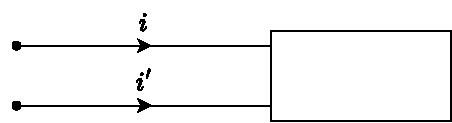
\includegraphics[width=0.35\textwidth]{assets/1,2/端口.drawio.pdf}
\caption{端口示意图}\label{端口示意图}
\end{figure}

与外部电路有 $n$ 个端口相连的电路称为 $n$ 端口网络(n-port network)。

部分常见的电路元件如图 \ref{部分常见电路元件} 所示(国家标准):

\begin{figure}[H]\centering
\begin{subfigure}[t]{0.52\textwidth}\centering
    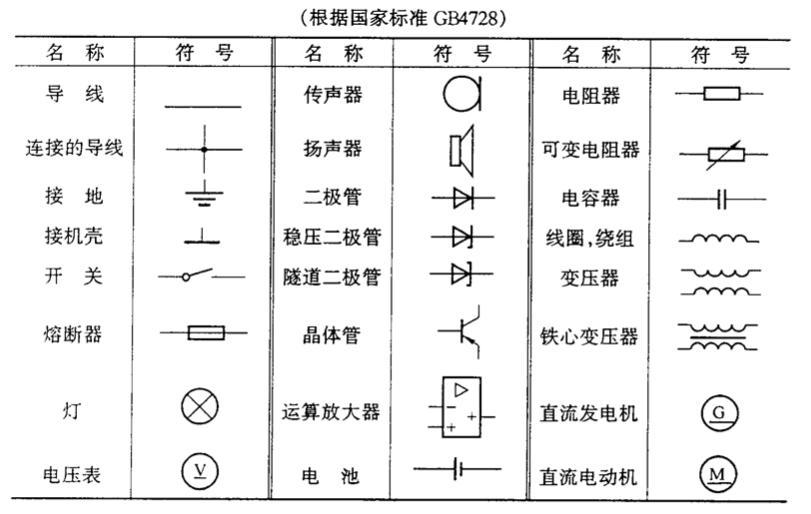
\includegraphics[height=160pt]{assets/1,2/7d3f6db847882c6447cc046186ede6ef.jpg}
\end{subfigure}\begin{subfigure}[t]{0.47\textwidth}\centering
    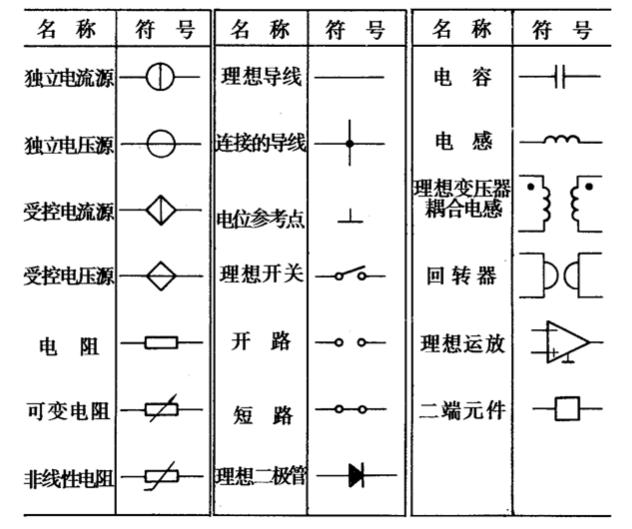
\includegraphics[height=160pt]{assets/1,2/3f5d73ec5ae9909ab42cd864852b0d72.jpg}
\end{subfigure}
\caption{部分常见电路元件}\label{部分常见电路元件}
\end{figure}





\section{电路分析基本观点}


\begin{definition}[建立电路模型]
电阻、电感与电容:
\begin{equation}
U = RI,\ \varPsi = LI,\ Q = CU
\end{equation}

$R, L, C$ 被称为电路基本模型,是电路分析的最基本模型。对不同的电路,应采用不同的模型,以适应实际需要并满足所需精度。另外,电路中常常使用大量的等效观点来简化电路的分析,使其求解更易、物理意义更清晰、应用更方便。

\end{definition}


\section{电路信号处理}

电路信号可分为图 \ref{信号分类、信号示意图} (a) 中的几类,它们的示意图如图 \ref{信号分类、信号示意图} (b) 所示: 

\begin{figure}[H]\centering
\begin{subfigure}[t]{0.52\textwidth}\centering
    \includesvg[height=75pt]{assets/1,2/信号分类.drawio.svg}
    \caption{ 信号分类 }
\end{subfigure}\begin{subfigure}[t]{0.48\textwidth}\centering
    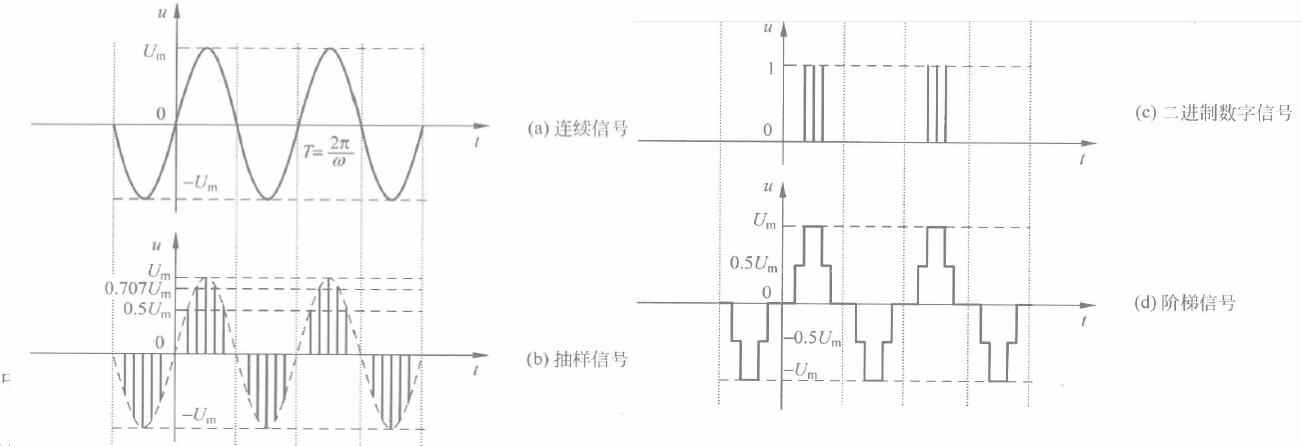
\includegraphics[height=75pt]{assets/1,2/1b9e0bed85e1f3a049de96f4c6018da8.jpg}
    \caption{ 信号示意图 }
\end{subfigure}
\caption{ 信号分类、信号示意图 }\label{信号分类、信号示意图}
\end{figure}

\section{电路能量处理}

\begin{definition}[功率]

二端元件吸收的瞬时功率(instantaneous power)为其单位时间内吸收的电能\footnote{在非关联参考方向下,瞬时吸收功率 $p = -ui$}:
\begin{equation*}
p(t) = \frac{\mathrm{d}w}{\mathrm{d}t} = \frac{\mathrm{d}w}{\mathrm{d}q}\cdot\frac{\mathrm{d}q}{\mathrm{d}t} = u(t)i(t) 
\end{equation*}


\begin{definition}[平均值、有效值]
对周期信号而言,其物理量有瞬时值、平均值、平均绝对值和有效值等特征量。以电压 $u = u(t)$ 为例:

\begin{enumerate}
\item 平均值(average value):$\bar{u} = \frac{1}{T}\int_0^T u(t)\mathrm{d}t$
\item 绝对平均值(average absolute value):$\overline{| u |} = \frac{1}{T}\int_0^T | u(t) |\mathrm{d}t$
\item 有效值(effective value):$ U = \sqrt{\frac{1}{T}\int_0^T u^2(t)\mathrm{d}t} $
\end{enumerate}
电流 $i$ 与上面同理。特别地,对正弦交流电流(sinusoidal altering current)而言,其有效值 $I = \frac{I_{\mathrm{m}}}{\sqrt{2}},\ U = \frac{U_{\mathrm{m}}}{\sqrt{2}}$。
\end{definition}


\end{definition}


\section{电路分类}


\begin{definition}[静态 / 动态电路]
    电路里,将可以提供能量或信号的元件称为源(source),将对能量或信号进行传输、分配和处理的元件称为负载(load)。
    负载全为电阻的电路称为电阻电路或静态电路,否则称为动态电路。前者需求解代数方程组,后者需求解微分方程组。本书第 2~4 章讨论静态电路,第 5~6 章讨论动态电路。
\end{definition}


\begin{definition}[线性 / 非线性电路]
判断是否线性需要先定义系统的激励(excitation)和响应(response),设激励为 $x$ 而响应为 $y = f(x)$,则系统是否线性由 $f$ 决定。例如电阻是二端线性系统,发光二极管是二端非线性系统。
\end{definition}


\begin{definition}[时变 / 非时变电流]
参数随时间变化的元件称为时变元件,含此类元件的电路称为时变电路,否则称为非时变电路。
\end{definition}


\begin{definition}[有源 / 无源电路]
对任意的一端口网络来说,设其端口电压 $u = u(t)$ 且 $u(0) = 0$ ,电流 $i = i(t)$ 且 $i(0) = 0$,该电路称为无源电路如果:
\begin{equation}
\int_{0}^{t} u(t)i(t)\mathrm{d}t \geqslant 0,\ \forall\ t >0
\end{equation}
否则称为有源电路,无源元件和有源元件同理。
\end{definition}


其它还可分为集总 / 分布参数电路、模拟 / 数字电路等。

\section{其它}




\begin{center}\noindent\begin{minipage}{0.65\textwidth}
    \begin{definition}[电路的基本名词]
    以图 \ref{电路基本名词} 为例:
    \begin{enumerate}
    \item 支路:若干元件无分岔地首尾相连构成一条支路。图里有三条支路(竖向的),因此 $p = 3$。
    \item 节点(node): 3个或更多支路的连接点。图中 $n = 4$。 
    \item 路径(path): 两个节点间包含的支路个数。
    \item 回路(loop): 由支路构成的闭合路径。图中 $l = 7$
    \item 网格(mesh): 平面电路中不与其余支路相交的回路,即最小网格数。图中 $m = 3$
    \end{enumerate}
    \end{definition}
\end{minipage}\hfill\begin{minipage}{0.35\textwidth}
    \begin{figure}[H]\centering
        \includesvg[width=\textwidth]{assets/1,2/电路基本名词.drawio.svg}
        \caption{电路基本名词}\label{电路基本名词}
    \end{figure}
\end{minipage}\end{center}





\chapter{简单电阻电路}\thispagestyle{fancy}
\section{电阻}
设一均匀线性电阻微元长 $\mathrm{d} l$,横截面积为 $\mathrm{d}S$,电阻率为 $\sigma$,则阻值为
\begin{gather}
    \mathrm{d}R = \frac{\mathrm{d} l}{\sigma\mathrm{d}S} \Longrightarrow R = \frac{L}{\sigma S} = \frac{\rho L}{S},\quad 
\text{串联:}\ R = \sum_{i}R_i,\quad 
\text{并联:}\ \frac{1}{R} = \sum_{i}\frac{1}{R_i} 
\end{gather}

多数金属材料的电阻率随温度变化见下式,其中 $\alpha$ 称为电阻温度系数,在实际使用时,最好保持额定功率在实际承受功率的两倍以上,以免过载。常见材料的具体数值见表 \ref{常见材料的0度电阻率和温度系数}。
\begin{equation}
\rho(T) = \rho_0(1+\alpha T)
\end{equation}
\begin{table}[H]\centering\small
    \setlength{\tabcolsep}{2mm} % 调整列间距
    \caption{常见材料的 0 \textdegree C 电阻率和温度系数}
    \label{常见材料的0度电阻率和温度系数}
    \resizebox{\linewidth}{!}{
        \begin{tabular}{cccccccccc}\toprule
            名称 & 银 & 铜 & 铝 & 钨 & 铁 & 碳 & 镍铬合金 & 镍铜合金\\
            \midrule
            $\rho_0\ (\Omega\cdot \mathrm{m})$
            &$1.5 \times 10^{-8}$ 
            &$1.6 \times 10^{-8}$ 
            &$2.5 \times 10^{-8}$ 
            &$2.5 \times 10^{-8}$ 
            &$8.7 \times 10^{-8}$ 
            &$3500 \times 10^{-8}$ 
            &$110 \times 10^{-8}$ 
            &$50 \times 10^{-8}$ \\
            $\alpha\ (\text{\textdegree C}^{-1})$
            &$4.0 \times 10^{-3}$ 
            &$4.3 \times 10^{-3}$ 
            &$4.7 \times 10^{-3}$ 
            &$4.6 \times 10^{-3}$ 
            &$5.0 \times 10^{-3}$ 
            &$-5.0 \times 10^{-4}$ 
            &$1.6 \times 10^{-4}$ 
            &$4.0 \times 10^{-5}$ \\
            \bottomrule
        \end{tabular}
    }
\end{table}


我们有欧姆定律微分形式和焦耳定律微分形式
\begin{equation}
i = \sigma E\ ,\ \ q =  \sigma E^2 = \frac{1}{\sigma} i^2  
\end{equation}

二极管模型如下,其中 $I_{\mathrm{S}}$ 为反向饱和电流(硅二极管典型值为 $10^{-12}$ A),$U_{TH}$ 为常数(典型值 25 mV)。
\begin{equation}
i = I_{\mathrm{S}}\left(e^{\frac{u}{U_{\mathrm{TH}}}} - 1\right)
\end{equation}

伏安特性曲线($u$-$i$ 特性曲线,voltage current relationship,VCR)的表达式为 $i = f(u)$ 或 $f(u,i) = 0$,
到目前为止,我们讨论的电阻 $u$-$i$ 特性曲线都在平面的一三象限(正电阻),后文我们将在等效观念指导下用运算放大器来实现负电阻性质。

\section{电源}


\begin{definition}[独立电源]
与外接电路无关的二端电源称为独立电源(independent source),例如独立电压源(independent voltage source)和独立电流源(independent current source)
\footnote{电压为零的独立电压源等效于短路,电流为零的独立电流源等效于断路}。
\end{definition}


\begin{definition}[受控电源]

流经元件的电压或电流受电路中其它部分电压或电流控制的元件称为受控电源。最常见的例子是放大器,如电子管、晶体管(又称三极管)等。
依据控制量和受控量的不同,受控电源一般分为 4 种:
\begin{itemize}
    \item 压控电压源(voltage controlled voltage source, VCVS)
    \item 流控电压源(current controlled voltage source, CCVS)
    \item 压控电流源(voltage controlled current source, VCCS)
    \item 流控电流源(current controlled current source, CCCS)
\end{itemize}
它们的电路符号如图 \ref{受控电源电路符号} 所示。 

\begin{figure}[H]\centering
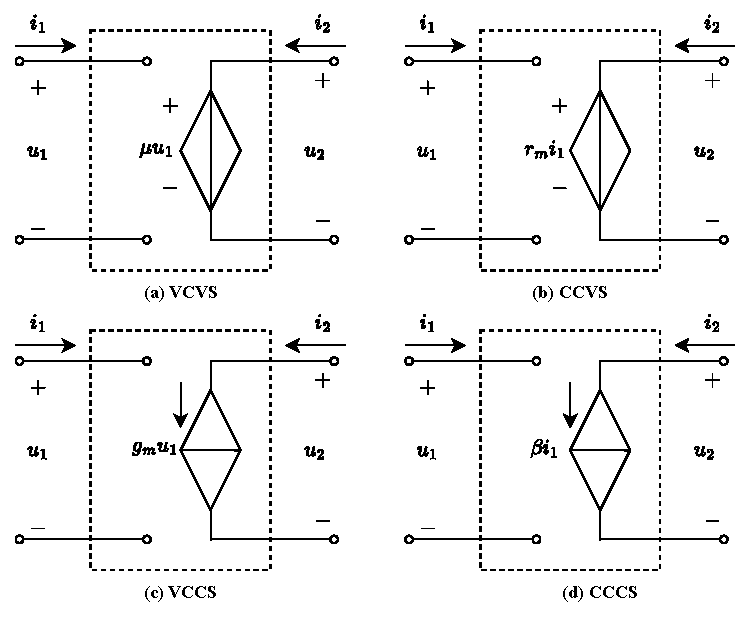
\includegraphics[width=0.7\textwidth]{assets/1,2/受控电源电路符号.drawio.pdf}
\caption{受控电源电路符号}\label{受控电源电路符号}
\end{figure}

图 \ref{受控电源电路符号} 中,控制量 $u_1$ 和 $i_1$ 分别是电路其它部分任意两点间的电压或电流;$\mu$ 是一个无量纲常数,称为电压放大倍数(转移电压比);$r_m$ 是电阻量纲常数,称为转移电阻;$g_m$ 是电导量纲常数,称为转移电导;$\beta$ 是无量纲常数,称为电流放大倍数(转移电流比)。

分析含受控源电路时需要注意,受控源性质和独立源有本质差别,不应简单等同。
\end{definition}



\section{基尔霍夫定律}


\begin{BlockTheorem}[基尔霍夫电流定律, KCL]
基尔霍夫电流定律(Kirchhoff's Current Law,KCL)表示,在任意时刻,电路中流入任一节点的电流代数和都为 0。
\begin{equation}
\sum i(t) = 0,\ \forall\ t 
\end{equation}
KCL 不仅适用于节点,对含多个端子的子电路也适用,称为广义 KCL。此定律本质上是是电流连续性 $\frac{\mathrm{d}q}{\mathrm{d}t} = 0$。

$n$ 节点电路含 $n-1$ 个独立的电流节点方程,构成第一方程组。
\end{BlockTheorem}

\begin{BlockTheorem}[基尔霍夫电压定律, KVL]
基尔霍夫电压定律(Kirchhoff's Voltage Law,KVL)表示,在任意时刻,沿任意回路的电压降(代数和)为 0。
\begin{equation}
\sum u(t) = 0,\ \forall\ t
\end{equation}
此定律本质上是法拉第电磁感应定律 $\oint \boldsymbol{E} \mathrm{d}\boldsymbol{l} = -\frac{\p \phi_B}{\p t} = 0$。

$n$ 节点 $p$ 支路的电路含有 $p-n+1$ 个独立的回路方程(即最小网格数),构成第二方程组。
\end{BlockTheorem}


\section{电路等效变换}

\subsection{电阻等效变换}

\noindent\textbf{平衡电桥:}

如图 \ref{平衡电桥与Y-Delta等效变换} (a),当 $\frac{R_1}{R_2} = \frac{R_3}{R_4}$ 时,$\varphi_A = \varphi_B$,AB 段无电流通过。 

\noindent\textbf{Y-$\Delta$ 等效变换:}

如图 \ref{平衡电桥与Y-Delta等效变换} (b),一般情况见下面公式。特别地,当三个电阻都相等时,我们有 $R_{\Delta} = 3R_Y$。
\begin{gather}
\boxed{
\begin{matrix}
    \text{由 Y 求 $\Delta$ :}\quad R_{12}= R_1 + R_2 + \frac{R_1R_2}{R_3}, \quad
    R_{13}=R_1 + R_3 + \frac{R_1R_3}{R_2} , \quad
    R_{23}=R_2 + R_3 + \frac{R_2R_3}{R_1} \\ 
    \text{由 $\Delta$ 求 Y :}\quad R_{1}=\frac{R_{12}R_{13}}{R_0}, \quad
    R_{2}=\frac{R_{21}R_{23}}{R_0}, \quad
    R_{3}=\frac{R_{31}R_{32}}{R_0},\quad 
    R_0 = R_{12}+R_{13}+R_{23} 
\end{matrix}
}
\end{gather}



\begin{figure}[H]\centering
\begin{subfigure}[t]{0.46\textwidth}\centering
    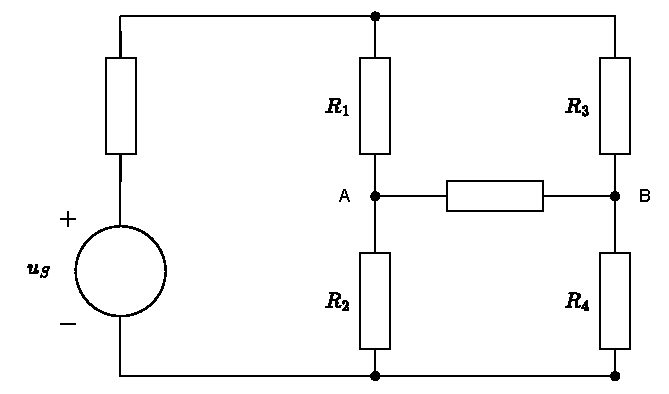
\includegraphics[height=125pt]{assets/1,2/平衡电桥.drawio.pdf}
    \caption{ 平衡电桥 }
\end{subfigure}\begin{subfigure}[t]{0.54\textwidth}\centering
    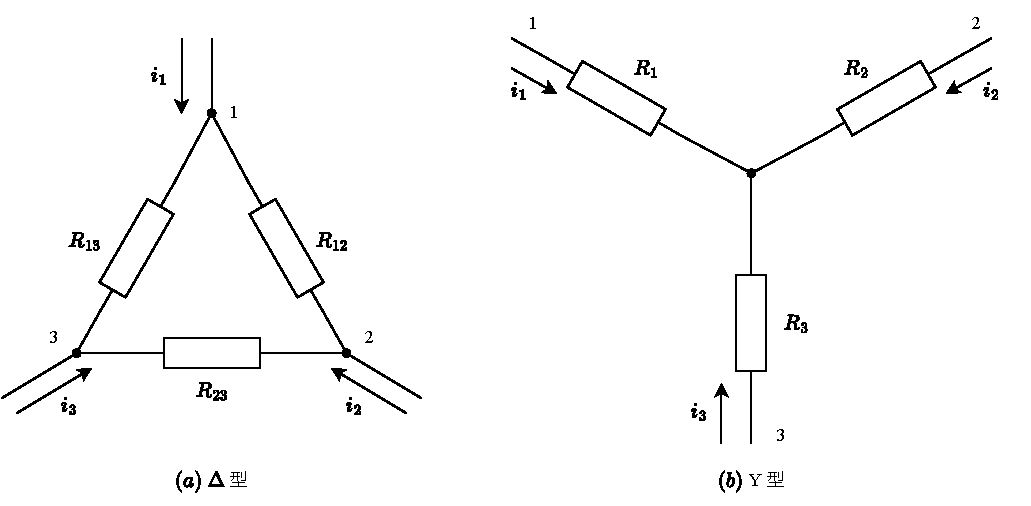
\includegraphics[height=125pt]{assets/1,2/YDelta等效变换.drawio.pdf}
    \caption{ Y-$\Delta$ 等效变换 }
\end{subfigure}
\caption{ 平衡电桥与Y-Delta等效变换 }\label{平衡电桥与Y-Delta等效变换}
\end{figure}

\subsection{电源等效变换}

含电阻和受控源的二端网络一般可等效为一个电阻。由于电路性质只与电路内部结构和参数有关,与外接激励无关,因此无论是外接独立电压源,还是外接独立电流源,都可以求出等效电阻。


\begin{definition}[独立源等效替换]
如图 \ref{实际独立源等效变换、独立电流源串联} (a),当满足下式时,两者可以等效替换 {\color{red}(注意变换前后的电流方向!)}。
\begin{equation}
U_S = I_SR_S\ \  \text{或}\ \  I_S = \frac{U_S}{R_S}
\end{equation}

例如,将电流源等效为电压源时,保持 $R_S$ 不变,令 $U_S = I_S R_S$ 即可;将电压源等效为电流源时,保持 $R_S$ 不变,令 $I_S = \frac{U_S}{R_S}$ 即可。

受控源可以像独立源一样进行等效变换,但要注意以下几点:
\begin{enumerate}
\item 对受控源作
等效变换时,如果变换只对受控量进行,则变换后仍是受控源,同时,不能将控制量所在支路变换掉
\item 当控制量与受控制量包含在一个二端网络内部时,可将此二端网络等效为一个电阻
\end{enumerate}
\end{definition}


\begin{definition}[独立电流源串联]
如图 \ref{实际独立源等效变换、独立电流源串联} (b) 所示,两个独立电流源串联,可以分别将其等效为独立电压源,等效仍成立。
\end{definition}

\begin{figure}[H]\centering
\begin{subfigure}[t]{0.53\textwidth}\centering
    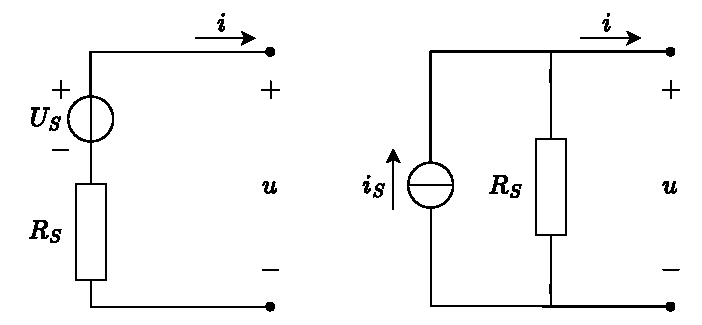
\includegraphics[height=120pt]{assets/1,2/独立源等效.drawio.pdf}
    \caption{ 实际独立源等效变换、独立电流源串联 }
\end{subfigure}\begin{subfigure}[t]{0.47\textwidth}\centering
    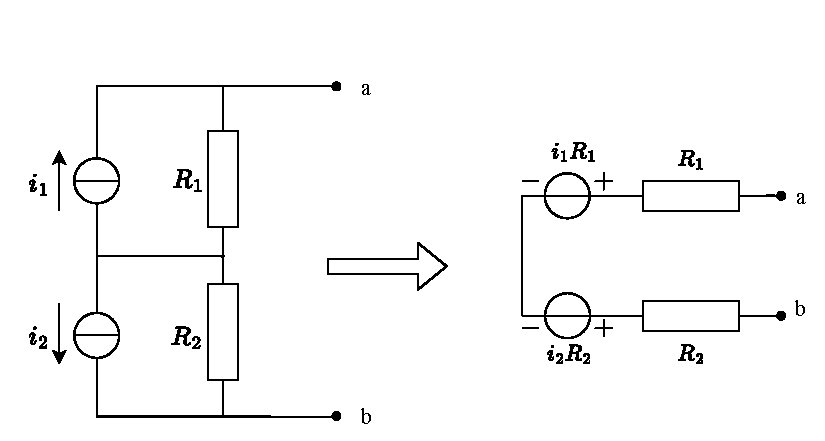
\includegraphics[height=120pt]{assets/1,2/独立电流源并联.drawio.pdf}
    \caption{ 独立电流源串联 }
\end{subfigure}
\caption{ 实际独立源等效变换、独立电流源串联 }\label{实际独立源等效变换、独立电流源串联}
\end{figure}


\begin{definition}[独立电压源并联]
如图 \ref{} 所示,两个独立电压源并联,可以分别将其等效为独立电流源,处理并联关系后转换为电压源,最终得:
\begin{equation}
U = \frac{\frac{U_1}{R_1} + \frac{U_2}{R_2}}{\frac{1}{R_1} + \frac{1}{R_2}} = \frac{R_2U_1 + R_1U_2}{R_1+R_2}, \quad R = \frac{R_1R_2}{R_1 + R_2}
\end{equation}

{\color{red} (缺图:独立电压源串联)}

\end{definition}



\begin{definition}[最大功率传输]
大多数仅含独立源和线性电阻的电路都可等效为一个实际独立电压源(内阻 $R_S$)外接一个负载电阻 $R_L$,则当且仅当 $R_S = R_L$ 时,$R_L$ 有最大功率。
\begin{equation}
P_L = P_L(R_L) =  \left(\frac{U_S}{R_S + R_L}\right)^2R_L, \ P_{L,\mathrm{max}} = P_L(R_S) = \frac{U_S^2}{4R_S}
\end{equation}
\end{definition}



\begin{definition}[元件与电压源并联]
如图 \ref{元件与电压源并联}  所示。理想电压源两端并联一个元件或一个网络,对电压源外部仍等效为一个理想电压源,即并联的这个元件或网络对原本的外电路求解没有任何影响。\footnote{例题见习题集:例 2-6}

\begin{figure}[H]\centering
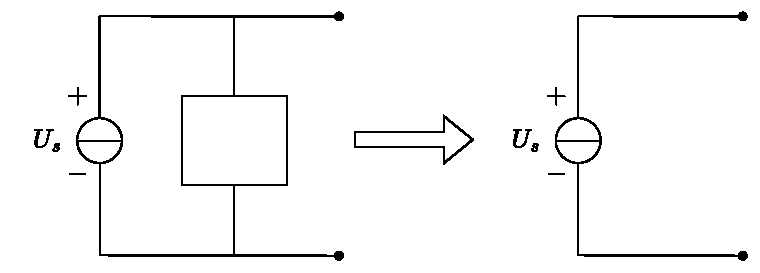
\includegraphics[width=0.5\textwidth]{assets/1,2/电阻与电源并联.drawio.pdf}
\caption{元件与电压源并联}\label{元件与电压源并联}
\end{figure}

例如,理想电压源 $U_s$ 的两端并联了一个电阻,对外等效结果是这个电阻不起作用。
\end{definition}

\begin{definition}[元件与电流源并联]
    类似地,理想电流源串联一个元件或一个网络,对电流源外部仍等效为一个理想电压源,即串联的这个元件或网络对原电路求解没有任何影响。\footnote{例题见习题集:例 2-7}
\end{definition}

\section{运算放大器}

\subsection{运算放大器 OPA 及其电气特性}


运算放大器(operational amplifier, Op Amp, OPA),简称运放,是一种性质特殊的多端集成电路,可视为电压放大器。借助 OPA,可实现模拟信号的各种数学运算。

在图 \ref{OPA 示意图} 中,OPA 的国标电路符号如图 (a) 所示,简化符号如图 (b) 所示,过去也惯用符号图 (c)。
\begin{figure}[H]\centering
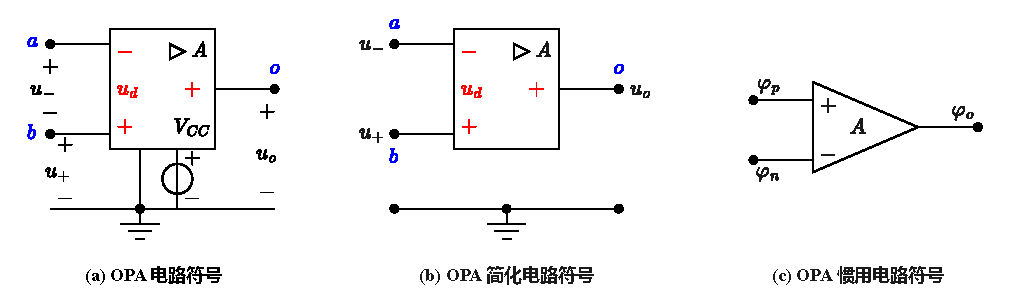
\includegraphics[width=0.8\textwidth]{assets/1,2/OPA运放.drawio.pdf}
\caption{OPA 示意图}\label{OPA 示意图}
\end{figure}

其中,a 接线端称为反相输入端(inverting input),用 $u_-$ 表示;b 接线端称为同相输入端(noninverting input),用 $u_+$ 表示;o 接线端称为输出端(output),用 $u_o$ 表示; $V_{CC}$ supply voltage, working voltage),向 OPA 提供直流电压以保证其正常工作;接地端 ground 并非大地,而是电源 $V_{CC}$ 的公共参考零点;参数 $A$ 为开环放大倍数。需要注意,在图 \ref{OPA 示意图} (b) 中,因为省略了电源部分,所以包围 OPA 的封闭曲线不满足广义 KCL。

OPA 的主要电气参数包括:
\begin{enumerate}
\item $V_\text{CC}$ : 供电电压(supply voltage)
\item $A$ : 差模电压增益(diffrential mode voltage gain),在开环情况下\footnote{(无输入引回到输出, diffrential mode)}满足 $u_o = Au_d = A(u_+-u_-) $,$A$ 因元件和温度而变,通常在 $10^5\sim 10^8$ 之间。
\item $R_i$ : 输入电阻(input resistance),$u_-$ 和 $u_+$ 端的等效电阻,基本上在 $\mathrm{M} \Omega$ 量级。
\item $R_o$ : 输出电阻(output resistance),$u_o$ 和接地端的等效电阻,基本上在 $\Omega$ 量级。
\item $U_{\text{sat}}$ : 饱和电压(saturate voltage),一般比 $V_{\text{CC}}$ 低两 $\mathrm{V}$ 左右。
\end{enumerate}

\noindent\begin{minipage}{0.67\textwidth}
\hspace{2em}OPA 仅在线性区内满足 $u_o = Au_d$,实际与近似输入输出曲线如图 \ref{OPA 输入输出曲线} 所示,在非线性区对外相当于一个独立电压源,称为正向(负向)饱和区。事实上,线性区是一个相当小的范围,例如 $A = 10^5$,$U_\text{sat} = 13 \V$,则 $U_{\text{ds}} = 0.13 \mV$。 
    
\hspace{2em}影响OPA的其它电气参数还包括输入失调电压、输入失调电流、输入偏置电流、压摆率(或转换速率)、增益宽带积、共模抑制比、静态功耗等。我们会在后续的模电课程中讨论它们对 OPA 的具体影响。
\end{minipage}\hfill
\begin{minipage}{0.31\textwidth}
    \begin{figure}[H]\centering
        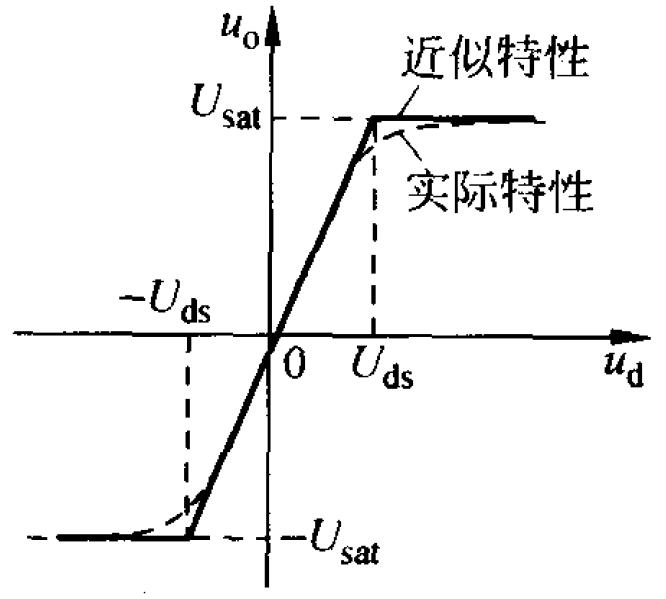
\includegraphics[width=\textwidth]{assets/1,2/image (49).jpg}
        \caption{OPA 输入输出曲线}\label{OPA 输入输出曲线}
        \end{figure}
\end{minipage}

由此可得出低频直流情形下 OPA 的低频受控源模型,如图 \ref{OPA 的低频受控源模型} (a) 所示。特别地,当电路电阻都在 $\kO$ 量级时,从工程的角度来看,可认为 $R_i = \infty$ 而 $R_o = 0$,如图 \ref{OPA 的低频受控源模型} (b) 所示。 

\begin{figure}[H]\centering
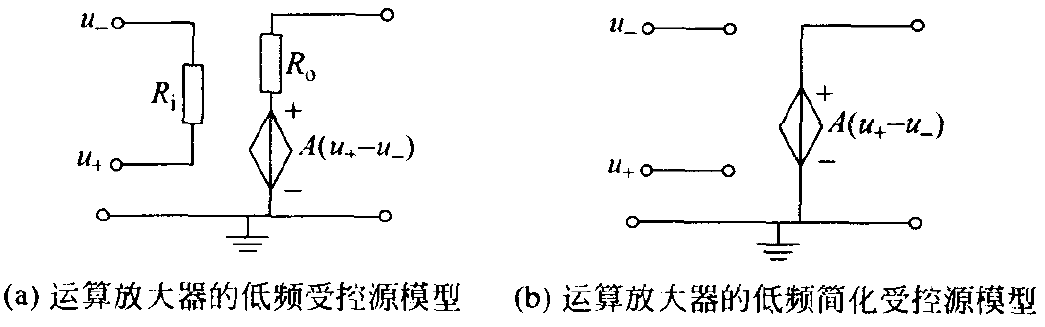
\includegraphics[width=0.7\textwidth]{assets/1,2/image (50).png}
\caption{OPA 的低频受控源模型}\label{OPA 的低频受控源模型}
\end{figure}

为了使 OPA 在多种场合可以正常使用,我们需要将一部分输出引回到输入,这种电路连接方式称为反馈(feedback)。将部分输出引到 $u_-$ 端,使得 $u_-$ 升高,进而抑制信号放大,可以构成负反馈;将部分输出引到 $u_+$ 端,使得 $u_+$ 升高,进而促进信号放大,可以构成正反馈。


先讨论一个负反馈的例子,如图 \ref{负反馈 OPA 电路} 所示,求电压放大倍数 $\frac{u_o}{u_i}$。

注意这里 $u_+ = 0$ 而 $u_- = u_i$,列出 KVL: 
\begin{gather}
u_i - iR_1 = u_1,\quad u_1 - iR_f = -Au_1 \Longrightarrow I =(1+A) \frac{u_1}{R_f} \\ 
\Longrightarrow \frac{u_o}{u_i} = \frac{-Au_1}{u_i} = \frac{-Au_1}{u_1+iR_1} = \frac{-A}{1+(1+A)\frac{R_1}{R_f}} = \frac{-AR_f}{AR_1 + (R_1 + R_f)}
\end{gather}
当电路电阻在 $\kO$ 量级,工程上可以认为:
\begin{equation}
\frac{u_o}{u_i} = -\frac{AR_f}{AR_1} = -\frac{R_f}{R_1}
\end{equation}
这样,信号放大倍数与 $A$ 无关,只需调整电阻值,即可得到合适的放大倍数。负反馈在保证 OPA 工作在线性区至关重要,同时,负反馈也可以很好的减弱噪声对输出信号的影响。有时希望 OPA 工作于饱和区,就需要引入正反馈。不加任何反馈的 OPA 也可用作电压大小的比较器。

\begin{figure}[H]\centering
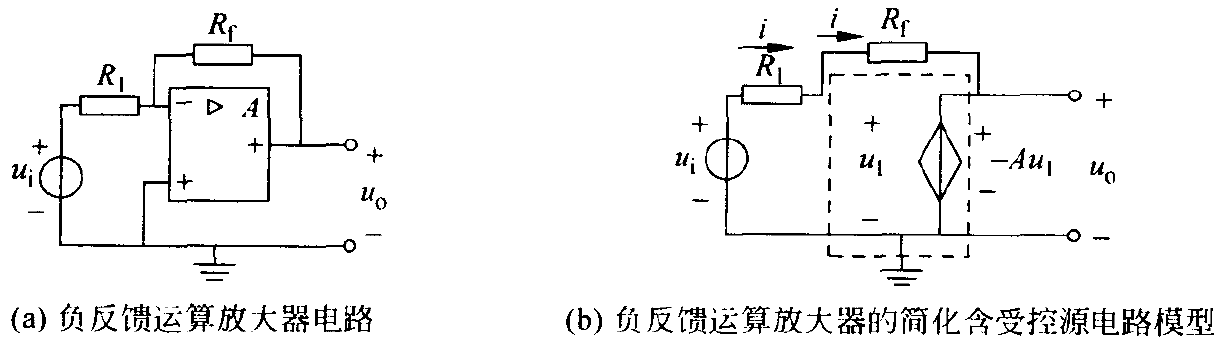
\includegraphics[width=0.75\textwidth]{assets/1,2/image (51).png}
\caption{负反馈 OPA 电路}\label{负反馈 OPA 电路}
\end{figure}


\subsection{理想放大器 IOPA}

\begin{definition}[理想限制条件]
一个 OPA 称为理想放大器(ideal operational amplifier, IOPA)如果它同时满足 $R_i = \infty,\ R_o = 0,\ A = \infty$\footnote{在模电课程中还会讨论 IOPA 的其它限制条件},其输入输出曲线如图 \ref{IOPA 输入输出曲线} 所示,用数学公式表示为:
\begin{equation}
\begin{cases}
    u_o \in (-U_{\text{sat}},\ +U_{\text{sat}}), &u_+ - u_i = 0 \\
    u_o = +U_{\text{sat}}, &u_+ - u_i > 0 \\
    u_o = -U_{\text{sat}}, &u_+ - u_i < 0 
\end{cases}
\end{equation}

对 IOPA 而言,始终有 $i_- = i_+ = 0$(因为 $R_i = \infty$),称为两条支路分别“虚断”。由于本小节讨论的 IOPA 始终处于线性区,因此有 $u_+ - u_- = 0 \Longrightarrow u_+ = u_- $,称为两点“虚短”。
\end{definition}

\begin{center}\noindent\begin{minipage}{0.4\textwidth}
        \begin{figure}[H]\centering
            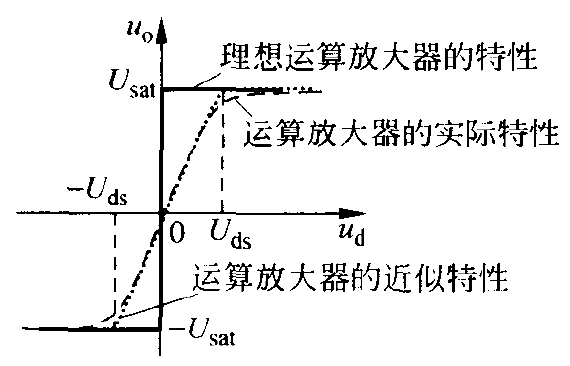
\includegraphics[height=100pt]{assets/1,2/4323bb51980c2d4d8e127dfa2e8110d0.png}
            \caption{IOPA 输入输出曲线}\label{IOPA 输入输出曲线}
        \end{figure}
    \end{minipage}\begin{minipage}{0.49\textwidth}
        \begin{figure}[H]\centering
            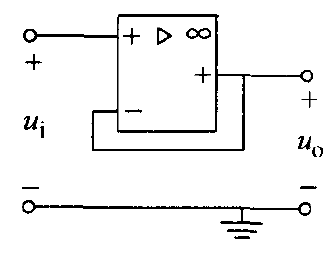
\includegraphics[height=100pt]{assets/1,2/电压跟随器.png}
            \caption{电压跟随器}\label{电压跟随器}
        \end{figure}
\end{minipage}\end{center}

\subsection{含 IOPA 的常见电路}
下面我们给出一些含 IOPA 的电路,在应用“虚断”、“虚断”下,推导是容易的,因此我们仅给出其电气特性而不给具体推导过程,除非某个推导较为困难。需要注意,运用“虚断”的前提是 OPA 的输入电阻 $R_{i} = \infty$,运用“虚短”的前提是放大倍数 $A = \infty$。在实际应用或解题时,必须验证输出电压 $u_o$ 是否在线性区内,否则“虚短”不再成立,且输出  $u_o = \pm U_{\text{sat}}$ 。

求输入电阻时,用加压求流法,也即已知输入电压 $u_i$,求输入电流 $i_{i}$,由 $u_i = i_iR_i$ 即得输入电阻。求输出电阻时,将独立源置零(这里电压源短路,成为导线),然后加流求压,由 $u = iR_o$ 得输出电阻。

% \usepackage{booktabs}


\begin{table}[H]
    \centering
    \caption{常见的含 OPA 电路}
    \begin{tabular}{ccccc} 
    \toprule
    名称         & 输入电阻 $R_i$ & 输出电阻 $R_o$ & 输出电压 $u_o$ & 专门特性  \\
    \hline
    电压跟随器      &   $\infty$   &    0  &   $u_i$   &   保电压,隔电路    \\
    同相比例放大器    &   $\infty$    &  0    &   $(1+\frac{R_1}{R_2})u_i$   &   放大电压    \\
    反相比例放大器    &    $R_1$  &   0   &  $-\frac{R_f}{R_l}u_i$    &  缺点是 $R_i = R_1$     \\
    反相加法器      &   $R_{i,k} = R_k,\ k = 1,2,3$   &   0   &   $-R_f\left( \frac{u_1}{R_1} + \frac{u_2}{R_2} + \frac{u_3}{R_3} \right)$   &    -   \\
    减法器        &   {\small $R_{i,1} = R_1, R_{i,2} = R_2 + R_M$}   &   0   &   $-\frac{R_f}{R_1}u_1 + \frac{1+\frac{R_f}{R_1}}{ 1 + \frac{R_2}{R_M}}u_2$   &  并减串加      \\
    电流源 VCCS &   $\infty$    &    0  &   $\left(  1+\frac{R_L}{R_1} \right)u_i$   &   $i_o = \frac{u_i}{R_1}$    \\
    负电阻        &   $-\frac{R_1}{R_2}R$   &   -   &   $\left(  1+\frac{R_2}{R} \right)u_i$   &    阻值  $-\frac{R_1}{R_2}R$  \\
    \bottomrule
    \end{tabular}
\end{table}

\begin{definition}[电压跟随器]
电压跟随器可以在保持电压的同时,有效地隔离电路,保持电路的独立性,利于电路设计。
\begin{enumerate}
\item 输入电阻:$R_i = \infty$
\item 输出电阻:$R_o = 0$
\item 电压特性:$u_o = u_i$
\end{enumerate}
\end{definition}

\begin{figure}[H]\centering
    \begin{subfigure}[t]{0.37\textwidth}\centering
        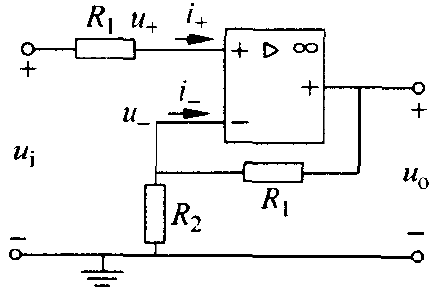
\includegraphics[height=90pt]{assets/1,2/同相比例放大器.png}
        \caption{ 同相比例放大器}
    \end{subfigure}\begin{subfigure}[t]{0.37\textwidth}\centering
        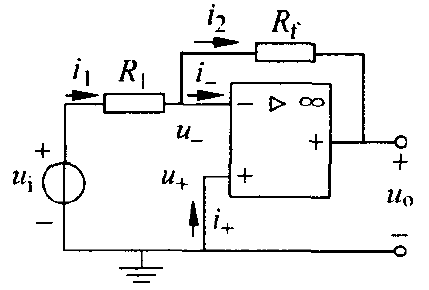
\includegraphics[height=90pt]{assets/1,2/反向比例放大器.png}
        \caption{ 反向比例放大器}
    \end{subfigure}
    \caption{ 比例放大器}
\end{figure}

\begin{definition}[同相比例放大器]
同相比例放大器能够放大输入信号,优点是输入电阻为 $\infty$ 且输出电阻为 0.
\begin{enumerate}
\item 输入电阻:$R_i = \infty$
\item 输出电阻:$R_o = 0$
\item 电压特性:$u_o = (1+\frac{R_1}{R_2})u_i$
\end{enumerate}
\end{definition}


\begin{definition}[反相比例放大器]
反相比例放大器的缺点是输入电阻为 $R_1$ 非无穷。
\begin{enumerate}
\item 输入电阻:$R_i = R_1$
\item 输出电阻:$R_o = 0$
\item 电压特性:$u_o = - \frac{R_f}{R_l} u_i$
\end{enumerate}
\end{definition}

\begin{figure}[H]\centering
    \begin{subfigure}[t]{0.37\textwidth}\centering
        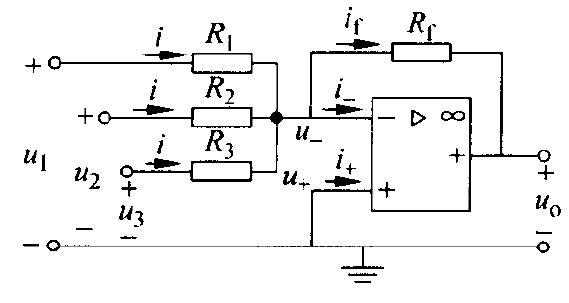
\includegraphics[height=90pt]{assets/1,2/反相加法器.png}
        \caption{ 反相加法器}
    \end{subfigure}\begin{subfigure}[t]{0.37\textwidth}\centering
        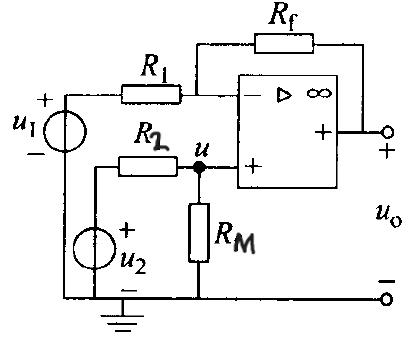
\includegraphics[height=90pt]{assets/1,2/减法器.png}
        \caption{ 减法器}
    \end{subfigure}
    \caption{ 反相加法器与减法器}
\end{figure}


\begin{definition}[反相加法器]
反相加法器的输入电阻平凡(非无穷),输出电阻为 0。
\begin{enumerate}
\item 输入电阻:$R_{i,1} = R_1,\ R_{i,2} = R_2,\ R_{i,3} = R_3$
\item 输出电阻:$R_o = 0$
\item 电压特性:$u_o = - R_f\left( \frac{u_1}{R_1} + \frac{u_2}{R_2} + \frac{u_3}{R_3} \right) $
\end{enumerate}
\end{definition}


\begin{definition}[减法器]
可以发现,减法器是在加法器的基础上,改变了 $u_+$ 端的电压而得。同理,向 $u_-$ 端并联电压源,或往 $u_+$ 端串联电压源,可以得到更普适的加减法器。但不能得到同相加法器,因为存在输入电阻为 0 的端口。
\begin{enumerate}
\item 输入电阻:$R_{i,1} = R_1,\ R_{i,2} = R_2 + R_M$
\item 输出电阻:$R_o = 0$
\item 电压特性:$u_o = -\frac{R_f}{R_1}u_1 + \frac{1+\frac{R_f}{R_1}}{1+\frac{R_2}{R_M}}u_2 $
\end{enumerate}
\end{definition}

\begin{figure}[H]\centering
\begin{subfigure}[t]{0.37\textwidth}\centering
    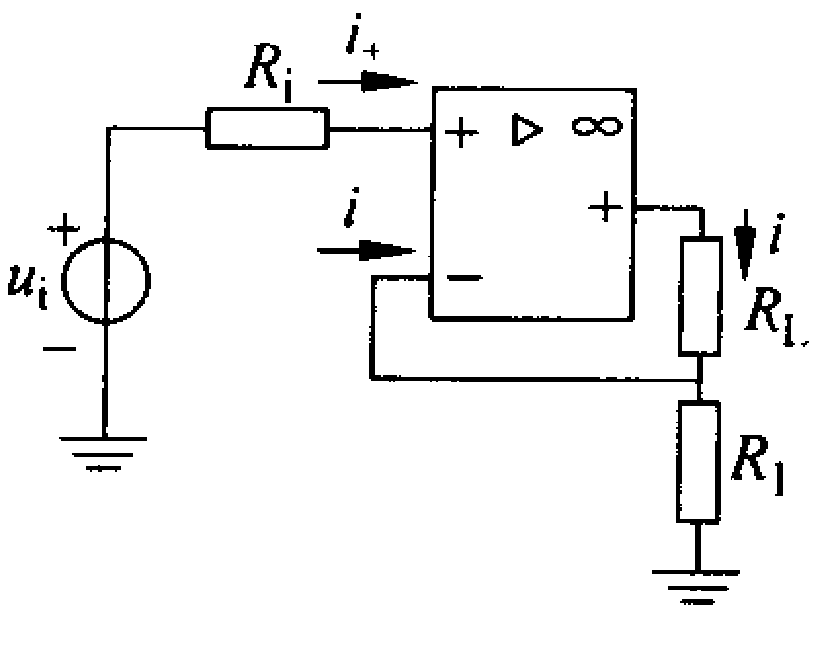
\includegraphics[height=95pt]{assets/1,2/压控电流源.png}
    \caption{ 压控电流源 VCCS}
\end{subfigure}\begin{subfigure}[t]{0.37\textwidth}\centering
    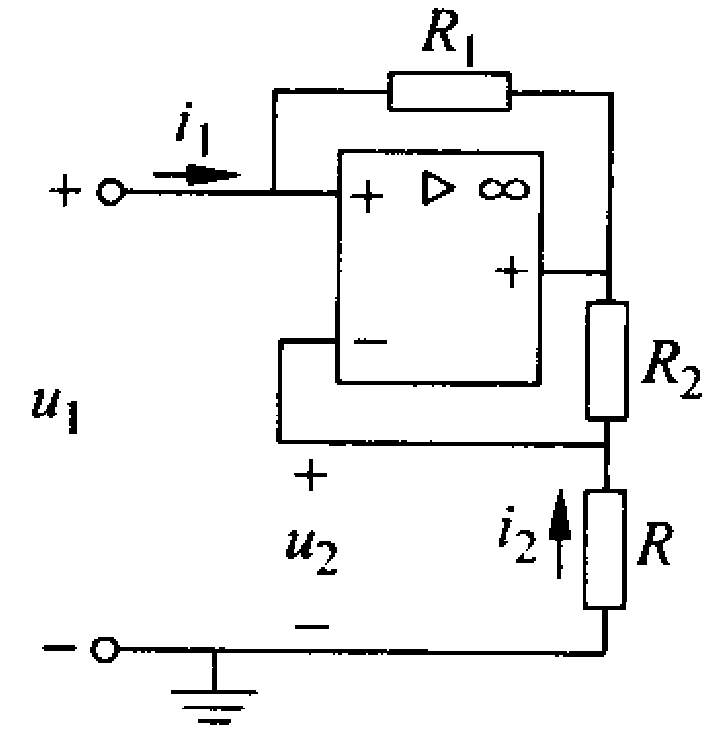
\includegraphics[height=95pt]{assets/1,2/负电阻.png}
    \caption{  负电阻}
\end{subfigure}
\caption{ 压控电流源 VCCS 和负电阻 }
\end{figure}


\subsubsection{压控电流源 VCCS: }
当输出电压 $u_o$ 在线性区时(受 $u_i$ 和负载 $R_L$ 影响),构成一个压控电流源。
\begin{enumerate}
\item 输出电流(负载电流):$i_o = \frac{u_i}{R_1}$
\item 输入电阻:$R_i = \infty$
\item 输出电阻:$R_o =  0$($R_L$ 两端是输出端)
\item 电压特性:$u_o = (1+\frac{R_L}{R_1})u_i$
\end{enumerate}


\begin{definition}[负电阻]
当输出电压 $u_o$ 在线性区时,构成一个负电阻(即输入电阻),在这里不存在输出电阻的概念。
\begin{enumerate}
\item 负电阻值(输入电阻):$R_i = -\frac{R_1}{R_2}R$
\item 电压特性:$u_o = (1+\frac{R_2}{R})u_i$
\end{enumerate}
\end{definition}

\subsection{其它含 OPA 的电路}

电压比较器、正反馈 IOPA、滞回比较器等,详见参考文献 \cite{电路原理} 的 Page 66。


\subsection{自设计线性运算器}
图 \ref{自设计线性运算器} 是在加法器、减法器的基础上,自己设计的线性运算器,它可以实现任意数量的输入(电压)信号的任意线性运算。事实上,在此线性运算器中,电阻 $R_M$ 和电阻 $R_P$ 是关键,因为在正相信号间的比例、反相信号间的比例分别确定时,这两个电阻实现了正信号和负信号之间的比例调整,使得最终输出的正、负信号可以任意大或任意小(最小即为 0,不占任何比例)。

图中,红色端是加法信号,蓝色端是减法信号,绿色端为公共地(可只保留一个)。

\begin{figure}[H]\centering
\begin{subfigure}[t]{0.49\textwidth}\centering
    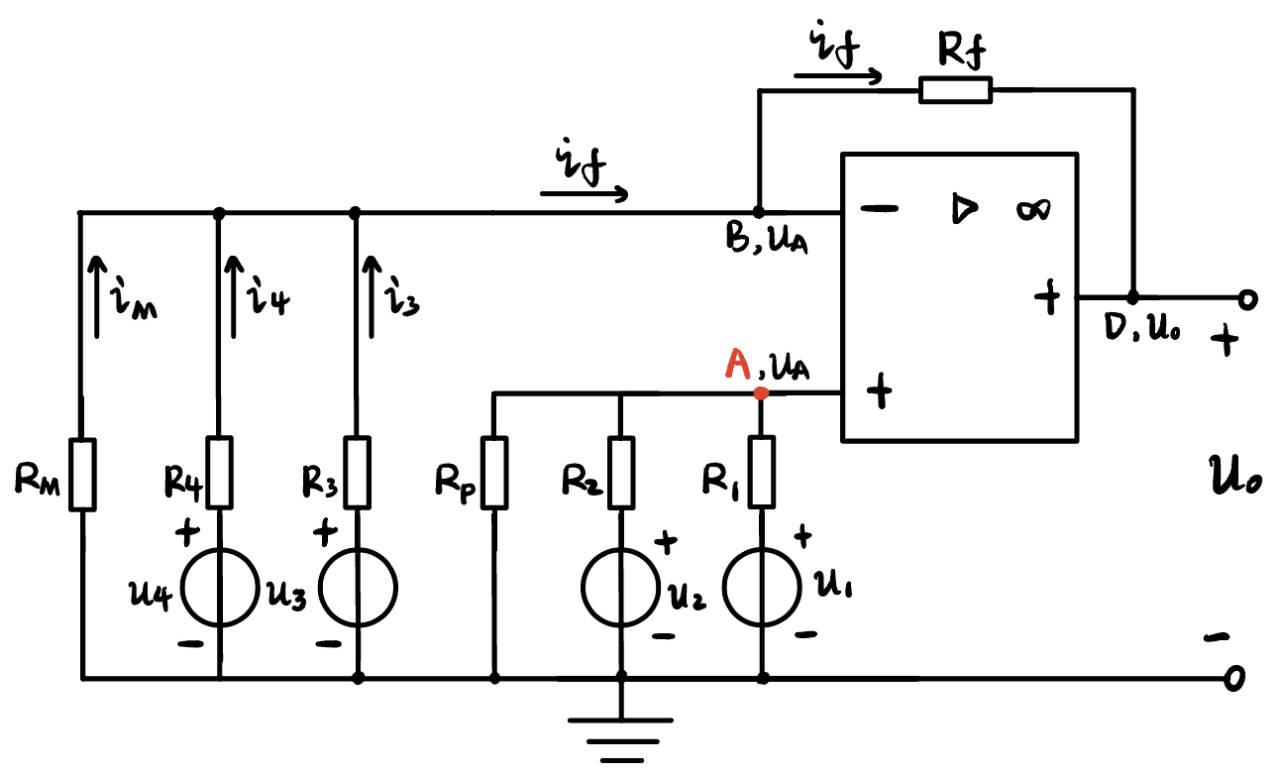
\includegraphics[height=140pt]{assets/1,2/线性运算器.png}
    \caption{ 线性运算器电路图 }
\end{subfigure}\begin{subfigure}[t]{0.49\textwidth}\centering
    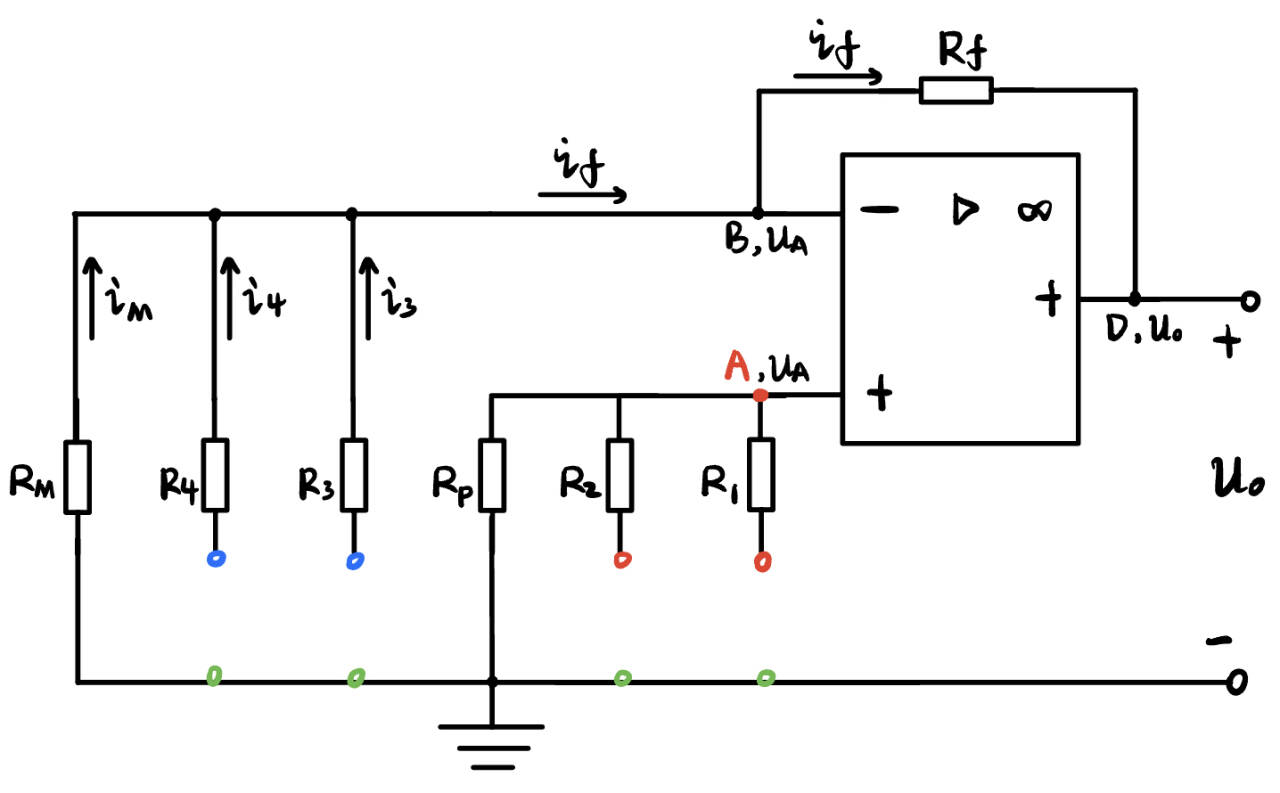
\includegraphics[height=140pt]{assets/1,2/线性运算器接线端.png}
    \caption{ 接线端示意图 }
\end{subfigure}
\caption{ 自设计线性运算器 }\label{自设计线性运算器}
\end{figure}


我们先研究图 \ref{自设计线性运算器} (a) 的输出特性,再讨论如果没有电阻 $R_M$ 或 $R_P$,输出电压会受到什么限制。输出电压的推导是简单的,先考虑点 A 的电势 $u_A$,求得:
\begin{equation}
u_A = \frac{\frac{u_1}{R_1} + \frac{u_2}{R_2}}{\frac{1}{R_1} + \frac{1}{R_2} + \frac{1}{R_p}}
\end{equation}

{\par\color{gray}\small
$u_A$ 的推导,除了列 KCL, KVL 硬解之外,还可以这样:先将 $R_p$ 断路,这样 $u_2, R_2, u_1, R_1$ 构成并联的两个实际电压源(自带电阻),容易求得此时点 A 的电势 $u_A$,并做数学上的形式变换:
\begin{equation}
u_A = \frac{R_2u_1 + R_1u_2}{R_1+R_2} =\frac{\frac{u_1}{R_1} + \frac{u_2}{R_2}}{\frac{1}{R_1} + \frac{1}{R_2} }
\end{equation}
于是,我们再并联一个实际电压源 P 后,由数学上直接推广,可以得到 $u_A$ 为:
\begin{equation}
    u_A = \frac{\frac{u_1}{R_1} + \frac{u_2}{R_2} + \frac{u_p}{R_p}}{\frac{1}{R_1} + \frac{1}{R_2} + \frac{1}{R_p}}
\end{equation}
再令 $u_p = 0$,即得图 \ref{自设计线性运算器} 中的原始 $u_A$。
\par}

再考虑左侧的电流组,并利用虚断:
\begin{align}
&\begin{cases}
    i_3 = \frac{1}{R_3}(u_3 - u_A) \\ 
    i_4 = \frac{1}{R_4}(u_4 - u_A) \\ 
    i_m = \frac{1}{R_m}(0 - u_A) \\ 
    i_f = i_3 + i_4 + i_m
\end{cases}
\Longrightarrow 
u_o = u_A - R_fi_f = u_A - R_f\left( i_3 + i_4 + i_m \right) \\ 
\Longrightarrow
u_o &=u_A - R_f \left[ 
\frac{u_3}{R_3} + \frac{u_4}{R_4} - u_A\left( \frac{1}{R_3} + \frac{1}{R_4} + \frac{1}{R_m} \right)
\right] \\ 
&=
\left[1 + R_f \left(\frac{1}{R_3} + \frac{1}{R_4} + \frac{1}{R_m} \right)\right] u_A - R_f \left( \frac{u_3}{R_3} + \frac{u_4}{R_4} \right) 
\end{align}
代入 $u_A$,整理得到:
\begin{equation}
\boxed{
    u_o= \frac{1 + \frac{R_f}{R_m} \left(\frac{1}{R_3} + \frac{1}{R_4}  \right)}{ \frac{1}{R_p} + \left(\frac{1}{R_1} + \frac{1}{R_2} \right)}\cdot \left( \frac{{\color{red} u_1}}{R_1} + \frac{{\color{red} u_2}}{R_2} \right) - R_f \cdot \left( \frac{{\color{red} u_3}}{R_3} + \frac{{\color{red} u_4}}{R_4} \right)
}
\end{equation}
这样,对于所有加法信号,可以通过 $R_1, R_2$ 间的比例来调整它们在加法中的输出比例,类似地,减法信号通过 $R_3, R_4$ 间的比例来调整它们在减法中的输出比例。最后通过 $R_f, R_m, R_p$ 来调整加法、减法之间的输出比例。在 $R_f, R_m, R_p$ 都可变时,易证(减法占比) $R_f \in [0,\ \infty)$,(加法占比)$\frac{1 + R_f \left(\frac{1}{R_3} + \frac{1}{R_4} + \frac{1}{R_m} \right)}{\frac{1}{R_1} + \frac{1}{R_2} + \frac{1}{R_p}} \in [0,\ \infty)$,于是全部系数都具有任意性,此线性运算器能够实现任意的线性运算。

上面的电路容易推广到任意输入信号个数的情形。假设有 $m$ 个加法信号 $u_{s_1}, \dots, u_{s_m}$,它们对应的串联电阻分别 $R_{s_1}, \dots, R_{s_m}$;以及$n$ 个减法信号 $u_{r_1}, \dots, u_{r_n}$,它们对应的串联阻值分别 $R_{r_1}, \dots, R_{r_n}$。直接由数学上推广出去,得到输出电压 
$u_o$ 的表达式为:

\begin{equation}
\boxed{
u_o = 
\left(
    \frac{1 + \frac{R_f}{R_m} + \displaystyle R_f\sum_{i=s_1}^{i=s_m} \frac{1}{R_i}
    }{
        \frac{1}{R_p} + \displaystyle \sum_{i=r_1}^{i=r_n} \frac{1}{R_i}
    }
\right)\cdot \displaystyle\sum_{i=s_1}^{i=s_m} \frac{{\color{red} u_i}}{R_i}  - R_f \cdot  \displaystyle\sum_{i=r_1}^{i=r_n} \frac{{\color{red} u_i}}{R_i}
}
\end{equation}

此线性运算器的具体仿真示例见 Homework 3.

\subsection{自设计线性运算器的两个关键电阻}

回到刚刚的问题,在图 \ref{自设计线性运算器} (a) 中,考虑没有电阻 $R_p$ 的情况,也即令 $R_p = \infty$。此时,对于给定的 $R_1, R_2, R_3, R_4$,减法总系数范围仍为 $[0,\ \infty)$,但加法的总系数范围却是 $[\frac{1}{R_1} + \frac{1}{R_2} ,\ \infty)$。

考虑两个电阻都没有的情况,令 $R_p = R_m = \infty$,则减法部分总系数为 1 不可改变,加法的总系数范围 $[\frac{1}{R_1} + \frac{1}{R_2} ,\ \infty)$

\subsection{OPA 实现指数对数乘法除法积分微分运算}

利用二极管可以实现指数和对数运算,乘法和除法由对数运算、线性运算、指数运算依次复合而成,引入电容可以实现积分、微分运算,详见 \href{https://zhuanlan.zhihu.com/p/628064125}{知乎:运算放大器的典型应用},这里不再赘述。特别地,引入电感还可以实现信号的相位移动。

关于 OPA 在 Multisim 中的仿真,可以参考 \href{https://space.bilibili.com/82683828}{Bilibili: 工程师看海} 的视频,以及仿真时的一些细节,我们不多赘述。

\section{二端口网络}

本 section 拓展阅读:
\begin{enumerate}
    \item \href{https://zhuanlan.zhihu.com/p/574470858}{知乎:二端口网络知识总结}
    \item \href{https://zhuanlan.zhihu.com/p/359677789}{知乎:从线性代数的角度理解线性二端口网络}
    \item \href{https://www.zhihu.com/question/357342024/answer/1477595759}{知乎:如何记住二端口ZYTH参数?}
\end{enumerate}

\subsection{二端口的概念与参数矩阵}


一个线性{\color{red} 无独立源}的四端网络称为二端口网络(two-port network)如果它的四个接线端构成两个端口,简称为二端口\footnote{需要注意,许多常见的含 OPA 电路都不构成端口(因为忽略了 OPA 的电源输入)。}。另外,有唯一公共端的 $n+1$ 端网络可以看作 $n$ 端口网络。
大多数时候,我们仅关心二端口的 $u$-$i$ 关系,其参数定义见表 \ref{参数矩阵代表的意义}。

相应地,表中矩阵参数表示的关系为:
\begin{gather}
\begin{bmatrix}
    i_1\\
    i_2\\
\end{bmatrix}
= 
\boldsymbol{G}
\cdot
\begin{bmatrix}
    u_1\\ 
    u_2\\
\end{bmatrix}
,\quad 
\begin{bmatrix}
    u_1\\
    u_2\\
\end{bmatrix}
= 
\boldsymbol{R}
\cdot
\begin{bmatrix}
    i_1\\ 
    i_2\\
\end{bmatrix}\quad 
\begin{bmatrix}
    u_1\\
    i_1\\
\end{bmatrix}
= 
\boldsymbol{T}
\cdot
\begin{bmatrix}
    u_2\\ 
    {\color{red} -i_2}\\
\end{bmatrix} 
,\quad 
\begin{bmatrix}
    u_1\\
    i_2\\
\end{bmatrix}
= 
\boldsymbol{H}
\cdot
\begin{bmatrix}
    u_2\\ 
    i_1\\
\end{bmatrix}
\end{gather}

\begin{table}[H]\centering
% \setlength{\tabcolsep}{1.5mm} % 调整列间距
    \caption{参数矩阵代表的意义}
    \label{参数矩阵代表的意义}
\begin{tabular}{cccccccccc}\toprule
    因变量& 自变量 & 参数矩阵 & 复参数名称\\
    \midrule
    $i_1, i_2$ & $u_1, u_2$ & 电导矩阵 $\boldsymbol{G}$ (conductance parameter) & $\boldsymbol{Y}$ 参数\\
    $u_1, u_2$ & $i_1, i_2$ & 电阻矩阵 $\boldsymbol{R}$ (resistance parameter) & $\boldsymbol{Z}$ 参数\\
    $u_1, i_1$& $u_2, i_2$&  传输矩阵 $\boldsymbol{T}$ (transmission parameter) & $\boldsymbol{T}$ 参数\\
    $u_1, i_2$& $u_2, i_1$&  混合矩阵 $\boldsymbol{H}$ (hybrid parameter matrix) & $\boldsymbol{H}$ 参数\\
    \bottomrule
\end{tabular}
\end{table}

其中 $\boldsymbol{R}$ 参数的 $R_{11}$ 和 $R_{22}$ 分别两个端口的输入电阻。
互易、对称二端口的概念不提,相关总结见图 \ref{二端口相关概念}。多个二端口网络级联\footnote{级联是二端口电路连接方式的一种,常见的连接方式有串联、并联、级联等,在后文会讨论}时,总参数矩阵是各网络参数矩阵的乘积。

需要特别注意的是,$\boldsymbol{T}$ 的互易条件是 $\det T = 1$ 而 $\boldsymbol{H}$ 的互易条件是 $H_{12} + H_{21} = 0$。

二端口吸收的功率 $p$ :
\begin{equation}
    \boxed{
        p = u_1i_1 + u_2i_2
    }
\end{equation}

另外,注意二端口两端输入电压的负极不一定等电势,也即 $u_1 = u_{1,+} - u_{1,-}$,$u_2 = u_{2,+} - u_{2,-}$,但不一定有 $u_{1,-} = u_{2,-}$。

\subsection{输入电阻与输出电阻}
\begin{LineTheorem}[戴维南定理]
一个含独立电源、线性电阻和受控源的一端口电路,对外可以等效成一个电压源和一个电阻串联,电压等于原电路端口两端的开路电压,电阻等于全部独立源置 0 (电压源短路,电流源断路)时的等效电阻。
\end{LineTheorem}

\begin{LineTheorem}[诺顿定理]
一个含独立电源、线性电阻和受控源的一端口电路,对外可以等效成一个电流源和一个电阻并联,电流大小等于原电路短路时端口流过的电流,电阻也是等于全部独立源置 0 (电压源短路,电流源断路)时的等效电阻。
\end{LineTheorem}

对二端口网络,计算输入电阻时,将输出端断开;计算输出电阻时,将输入端置零(用一根导线替代电源,若没有电源则相连)。

\newpage
\begin{figure}[H]\centering
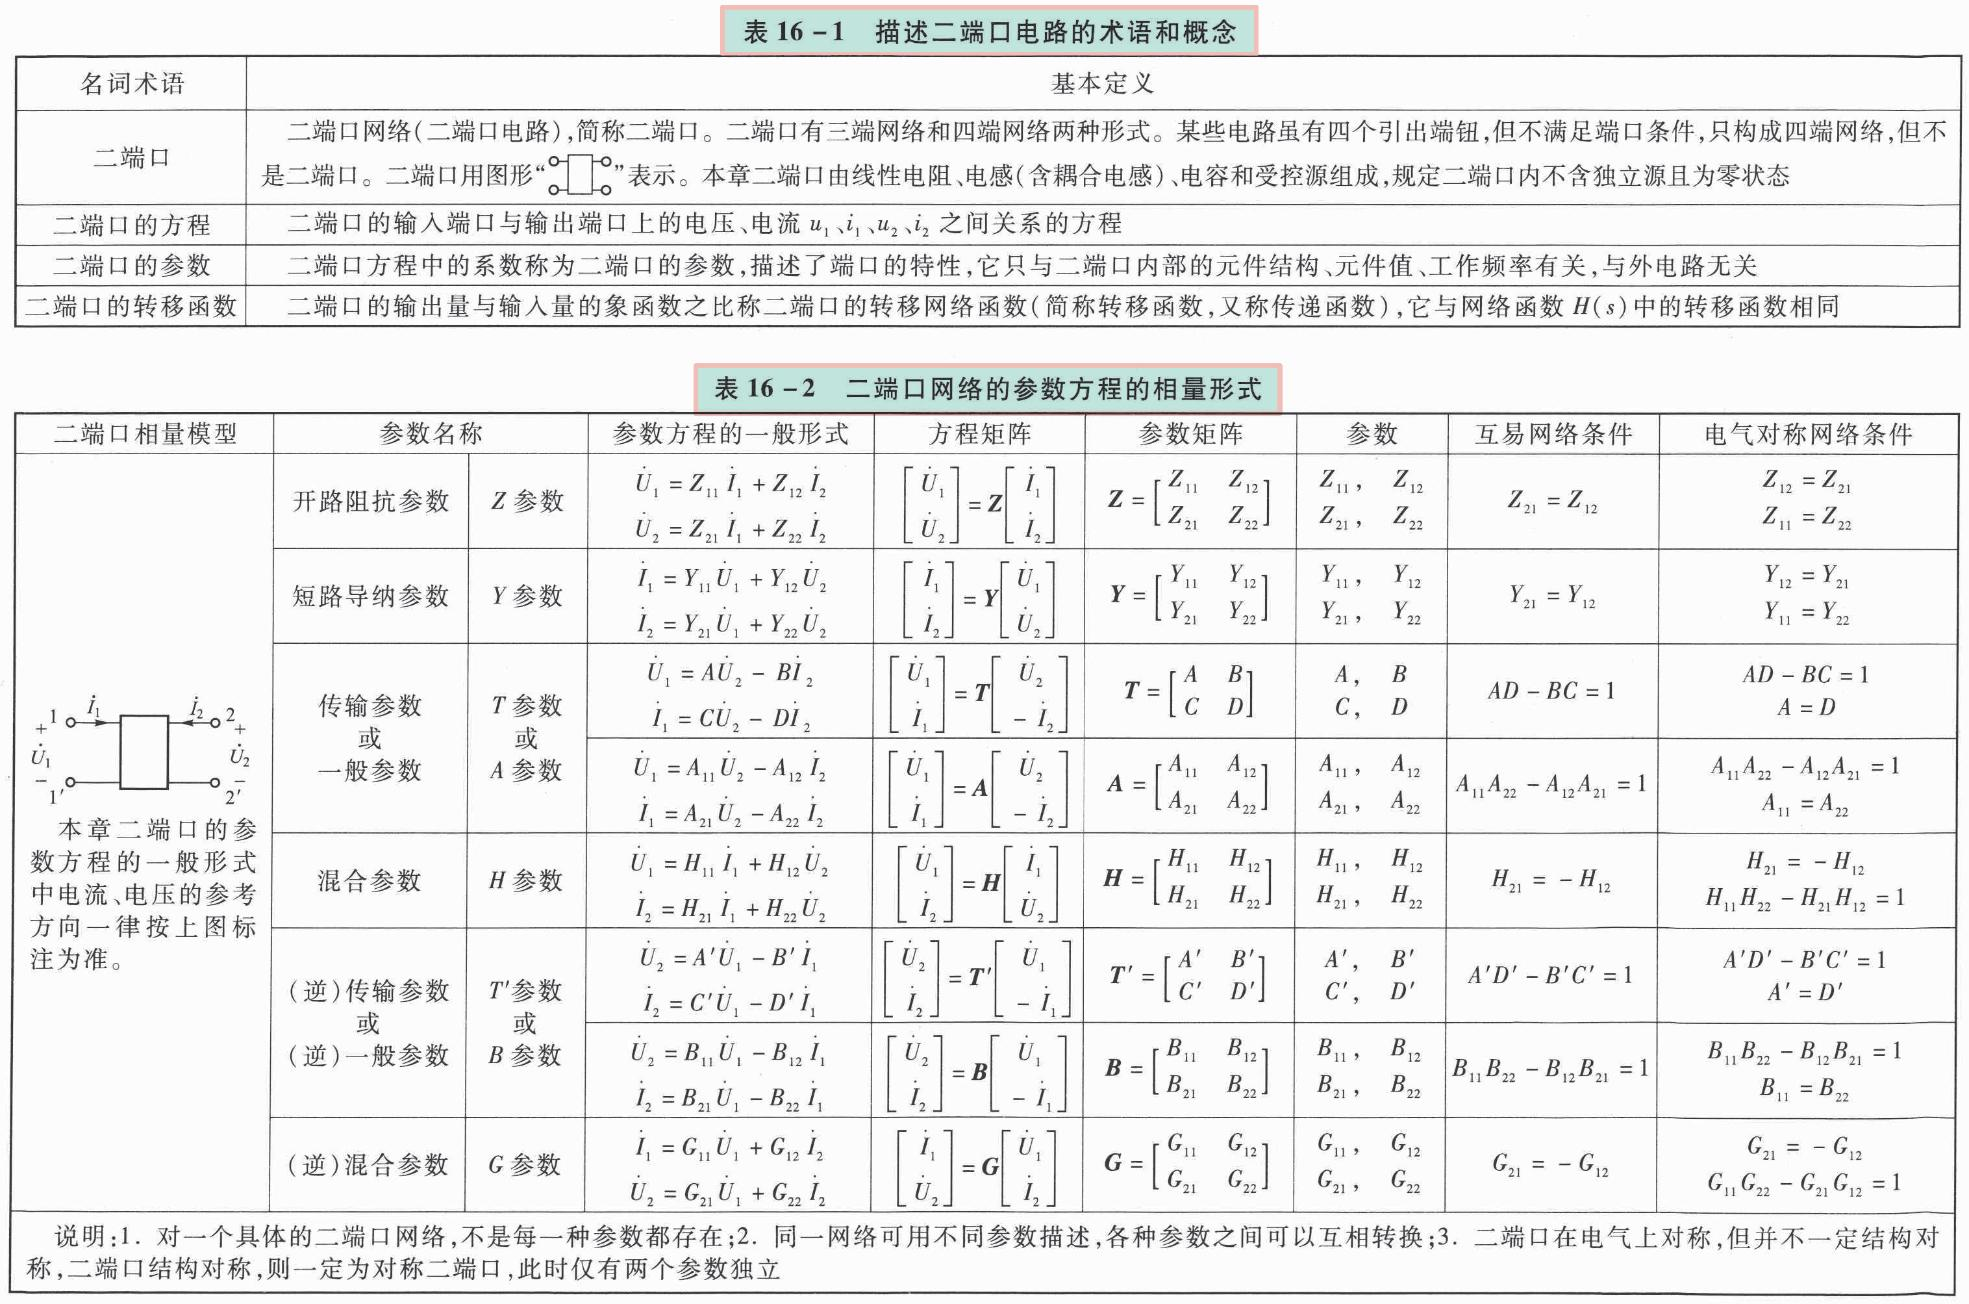
\includegraphics[width=\textwidth]{assets/1,2/二端口网络.jpg}
\caption{ 二端口相关概念}\label{二端口相关概念}
\end{figure}

\begin{figure}[H]\centering
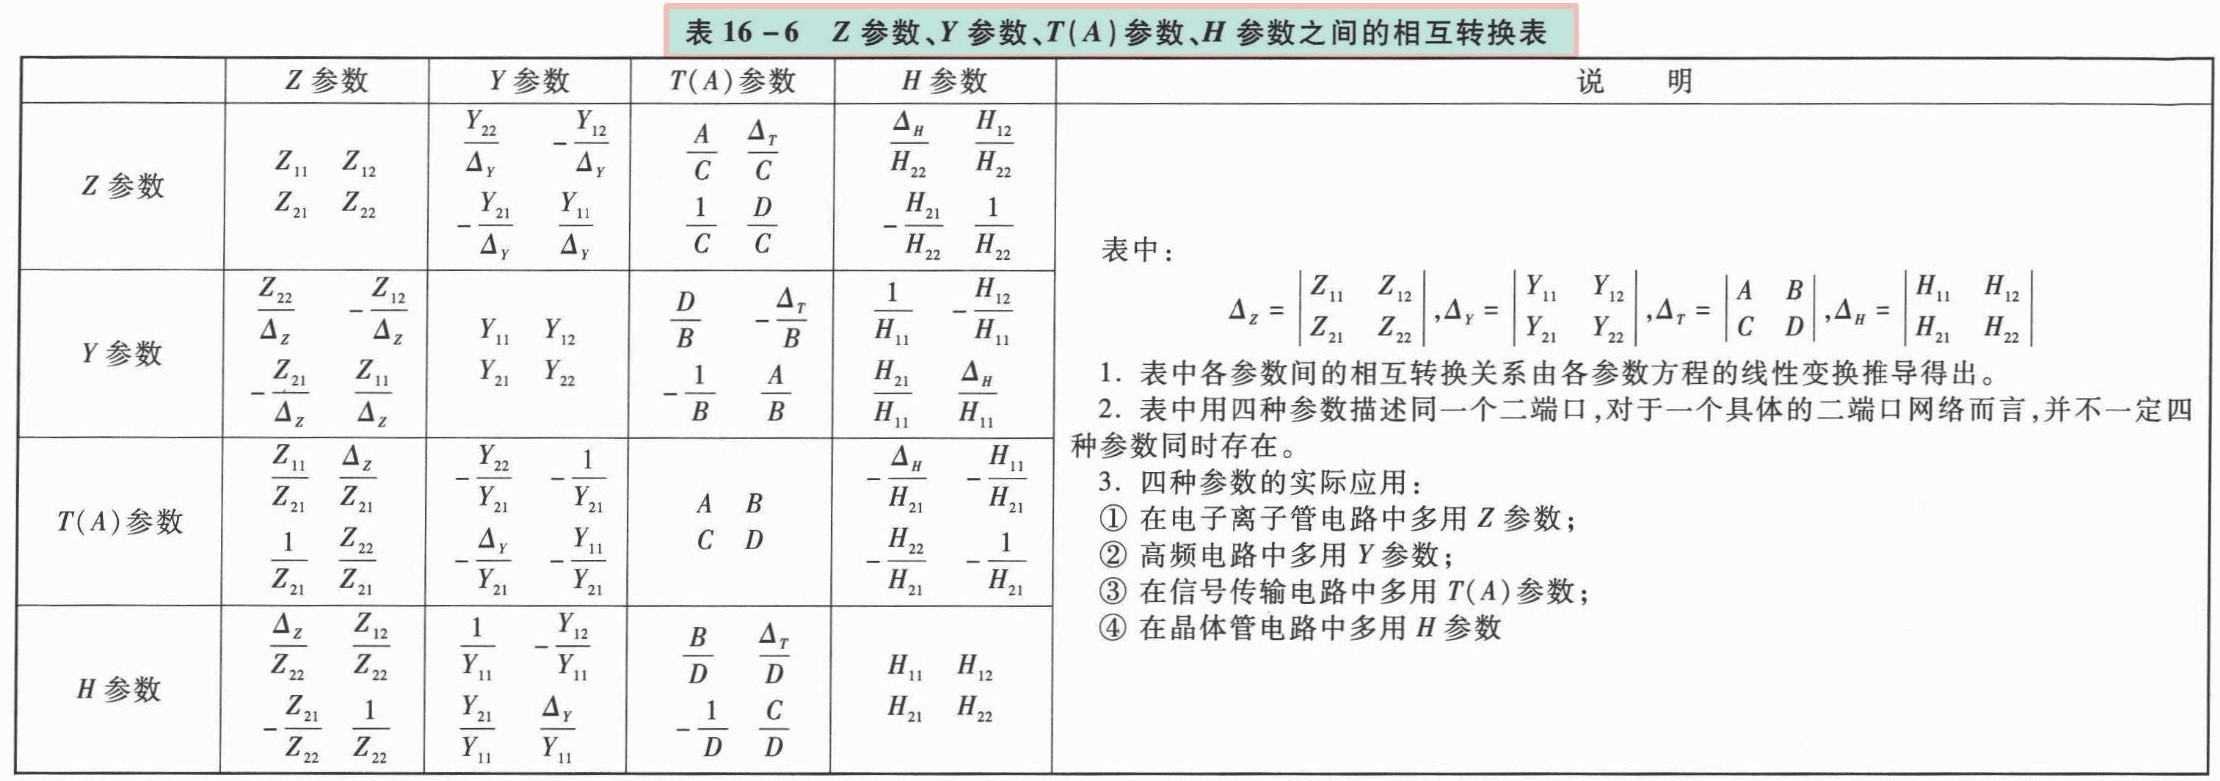
\includegraphics[width=\textwidth]{assets/1,2/image (9).jpg}
\caption{ 参数矩阵间的关系与等效电路}\label{参数矩阵间的关系与等效电路}
\end{figure}

\subsection{二端口的常见联接方式}

必须指出的是,在二端口进行联接时,子二端口的端口条件可能被破坏,称为非正规联接,此时不能应用下面的结论计算电路参数。级联一定是正规联接,但其它联接方法是否正规,需要进行判断。若为白箱,可通过推导判断,若为黑箱,需通过实验验证端口条件,具体的验证方法见参考文献 \cite{电路原理导学导教} 的 Page 23,我们不多赘述。

另外,在计算各参数矩阵的值时(尤其是 $\boldsymbol{T}$、$\boldsymbol{H}$ 参数),一定不要忘记在最终数值结果中写上单位。

\begin{table}[H]\centering
    %\renewcommand{\arraystretch}{1.5} % 调整行间距为 1.5 倍
    %\setlength{\tabcolsep}{1.5mm} % 调整列间距
    \caption{二端口的六种常见连接方式}
    \label{二端口的六种常见连接方式}
\begin{tabular}{cccccccccc}\toprule
    连接方式 & 参数矩阵 & 连接方式 & 参数矩阵 & 连接方式 & 参数矩阵\\
    \midrule
    级联  &  $\boldsymbol{T} = \boldsymbol{T_1}\cdot \boldsymbol{T_2}$    &   串联 & $\boldsymbol{R} = \boldsymbol{R_1} \cdot \boldsymbol{R_2}$ & 串并联 & $\boldsymbol{H} = \boldsymbol{H_1} + \boldsymbol{H_2}$ \\ 
    负级联 &  $\boldsymbol{T} = -\boldsymbol{T_1}\cdot \boldsymbol{T_2}$  &   并联 & $\boldsymbol{G} = \boldsymbol{G_1}\cdot \boldsymbol{G_2}$ & 并串联 & $\boldsymbol{H^{-1}} = \boldsymbol{H_1^{-1}} + \boldsymbol{H_2^{-1}}$\\ 
    \bottomrule
\end{tabular}
\end{table}

\begin{figure}[H]\centering
\begin{subfigure}[t]{0.42\textwidth}\centering
    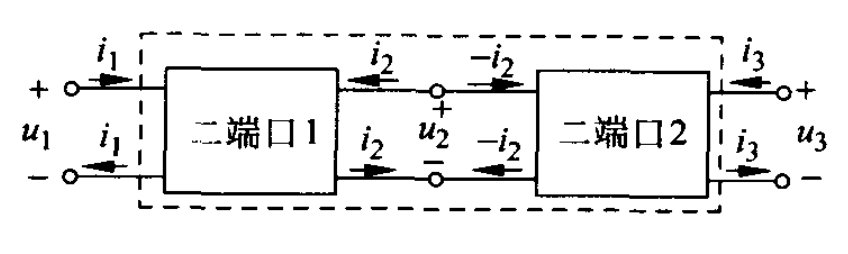
\includegraphics[height=60pt]{assets/2/级联.png}
    \caption{ 级联 }
\end{subfigure}\begin{subfigure}[t]{0.58\textwidth}\centering
    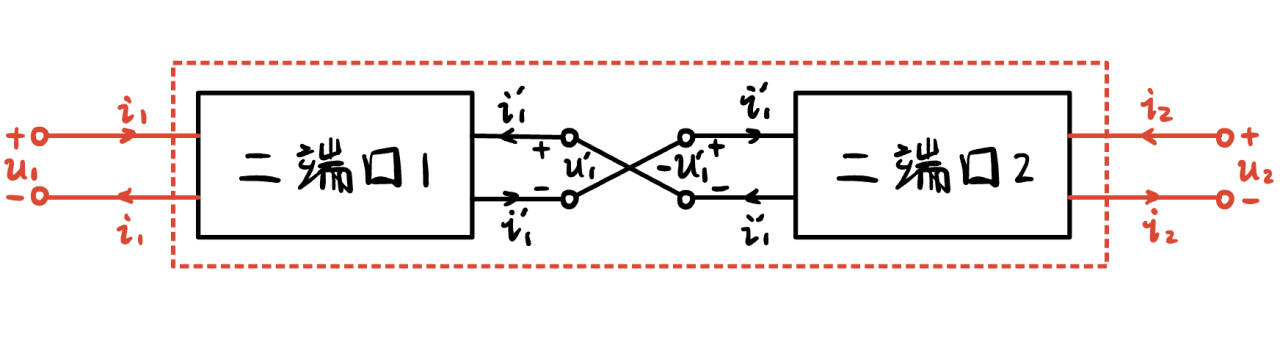
\includegraphics[height=60pt]{assets/2/负级联.png}
    \caption{ 负级联 }
\end{subfigure}
\caption{ 二端口级联、负级联}
\end{figure}

\begin{figure}[H]\centering
\begin{subfigure}[t]{0.46\textwidth}\centering
    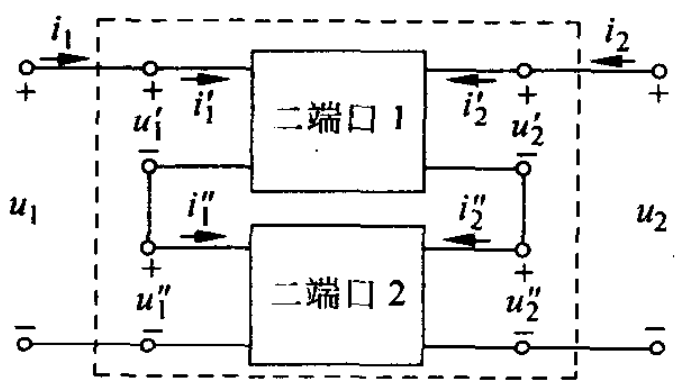
\includegraphics[height=120pt]{assets/2/串联.png}
    \caption{ 串联 }
\end{subfigure}\begin{subfigure}[t]{0.54\textwidth}\centering
    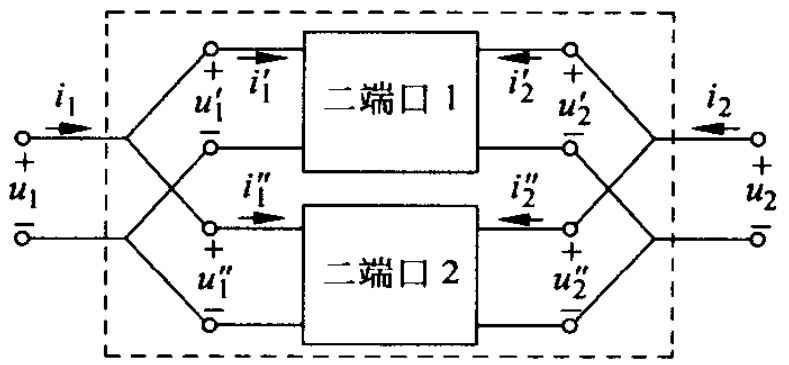
\includegraphics[height=120pt]{assets/2/并联.png}
    \caption{ 并联 }
\end{subfigure}
\caption{ 二端口串联、并联 }
\end{figure}

\begin{figure}[H]\centering
\begin{subfigure}[t]{0.5\textwidth}\centering
    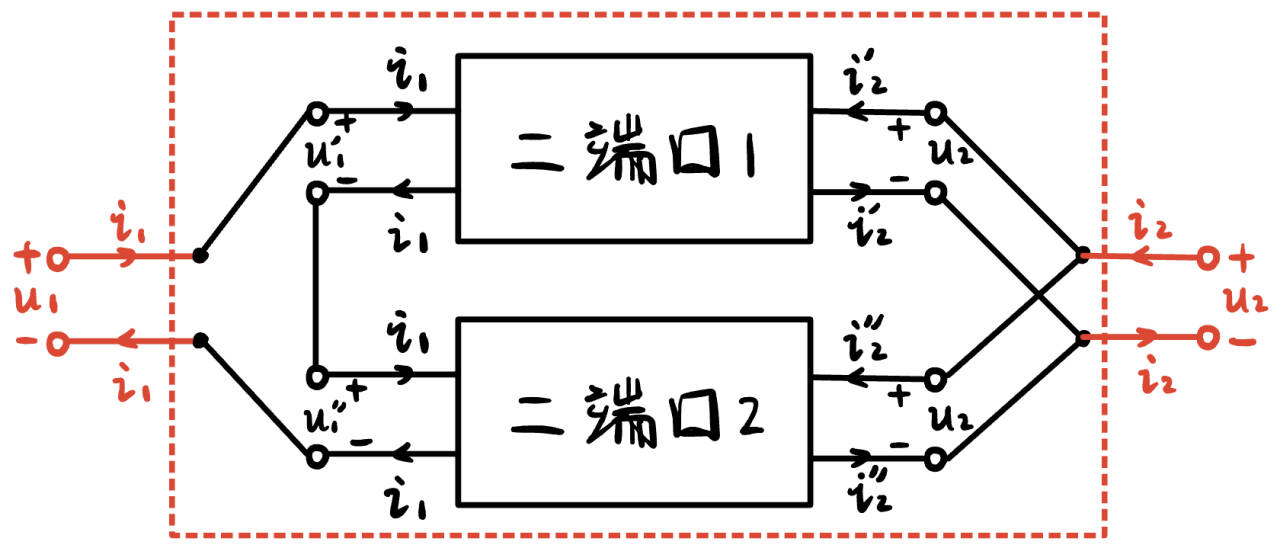
\includegraphics[height=100pt]{assets/2/串并联.png}
    \caption{ 串并联 }
\end{subfigure}\begin{subfigure}[t]{0.5\textwidth}\centering
    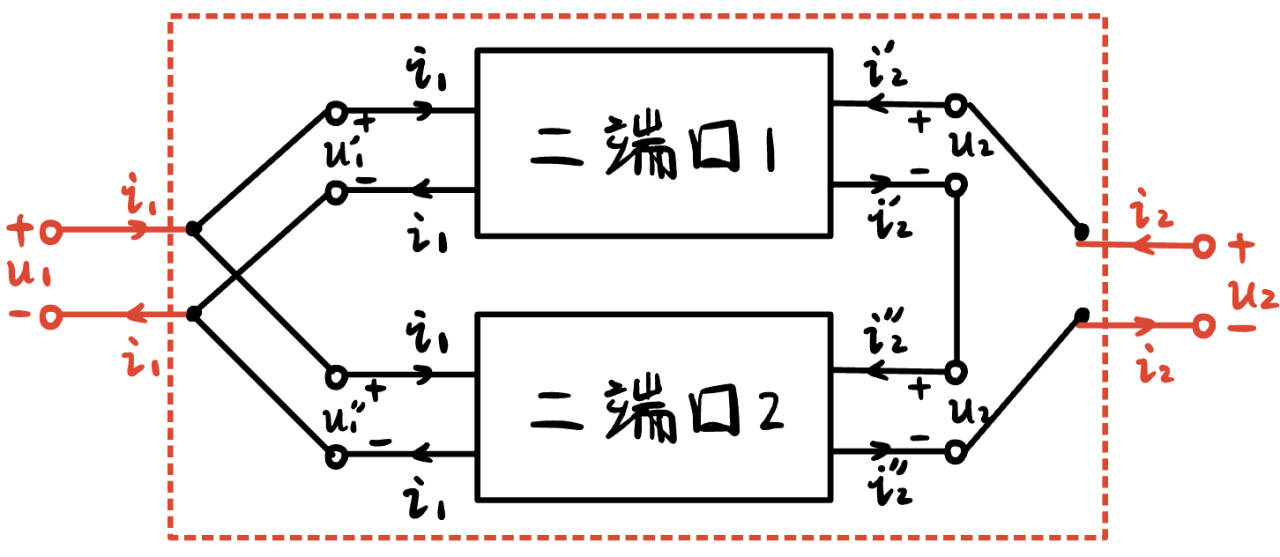
\includegraphics[height=100pt]{assets/2/并串联.png}
    \caption{ 并串联 }
\end{subfigure}
\caption{ 二端口串并联、并串联 }
\end{figure}

\subsection{参数矩阵间的转换与等效电路}
$\boldsymbol{G}$ 与 $\boldsymbol{R}$ 矩阵之间满足 $\boldsymbol{G}^{-1} = \boldsymbol{R}$(如果可逆),其它关系见图 \ref{参数矩阵间的关系与等效电路}。

{\color{red} 不含独立源}的二端口网络一定可以被等效,满足所需的参数矩阵相同即可。特别地,若二端口满足互易条件,则可以等效为一个三电阻电路。特别注意,$\boldsymbol{T}$ 参数等效时 ${\color{red} R_T = \frac{1}{T_{21}} \ne}  \frac{1}{T_{21}}$。
\begin{equation}
\begin{matrix}
    \text{$\boldsymbol{R}$ 互易, T 型等效} \\ 
    \begin{cases}
        R_T = R_{12} = R_{21} \\ 
        R_1 = R_{11} - R_T \\ 
        R_2 = R_{22} - R_T 
    \end{cases}
\end{matrix},\quad 
\begin{matrix}
    \text{$\boldsymbol{G}$ 互易, $\pi $ 型等效} \\ 
    \begin{cases}
        G_{\pi} = -G_{12} = -G_{21} \\ 
        G_1 = G_{11} - G_{\pi} \\ 
        G_2 = G_{22} - G_{\pi} \\ 
    \end{cases}
\end{matrix}\quad 
\begin{matrix}
    \text{$\boldsymbol{T}$ 互易, T 型等效} \\
    \begin{cases}
        {\color{red} R_T = \frac{1}{T_{21}}}\\ 
        R_1 = R_T(T_{11} -1) \\ 
        R_2 = R_T(T_{22} -1) \\ 
    \end{cases}
\end{matrix}
\end{equation}



\begin{center}\noindent\begin{minipage}{0.58\columnwidth}
    \hspace*{2em} 普遍的等效需要受控源,参数 $\boldsymbol{G}$ 和 $\boldsymbol{S}$ 的等效详见参考文献 \cite{电路原理} Page 79,这里只提 $\boldsymbol{T}$ 和 $\boldsymbol{H}$ 如何等效。等效的思路是相同的,都是得到两个因变量的表达式,一个端口各一个(例如 ($u_1, u_2$) 或者 $(u_1, i_2)$),这样便将电路分为了两部分,分别用受控源和电阻进行等效即可。

    \hspace*{2em} 已知 $\boldsymbol{T}$ 参数时,依据参数转换关系求出 $\boldsymbol{H}$ 参数,以得到表达式 $u_1 = u_1(u_2,i_1), i_2 = i_2(u_2,i_1)$,此时可以等效为右图电路。
\end{minipage}\hfill\begin{minipage}{0.39\columnwidth}
    \begin{figure}[H]\centering
        \includesvg[width=\columnwidth]{assets/2/H参数等效.svg}
        \caption{$H$ 参数等效电路}\label{H参数等效电路}
    \end{figure}
\end{minipage}\end{center}



\section{MOSFET(金属氧化物半导体场效应晶体管)}

\subsection{MOSFET 基本概念}

MOSFET,是指 Metal Oxide Semiconductor Field Effect Transistor,它是数字电路的核心元素。小功率 FET 有 JFET、MOSFET,大功率 FET 有 VDMOS、IGBT 等,本课程主要面向 MOSFET。


\begin{center}\noindent\begin{minipage}{0.41\columnwidth}
    \hspace*{2em} 图 \ref{} 是 N-MOS 和 P-MOS 的符号(ANSI 标准),其中 N MOS 的箭头朝内(因为 Negative)电流方向是 D > S;P MOS 的箭头朝外(因为 Positive),电流方向是 S > D。

    \hspace*{2em} 需要特别强调的是,部分教材中会采用图 \ref{} 中的简化版 MOS 符号(例如参考文献 \cite{电路原理} \cite{电路原理导学导教}),一定注意这种符号的 {\color{red} 箭头朝向与简化前相反}!除非特殊情况,本文一律使用 ANSI 标准的符号。
\end{minipage}\hfill\begin{minipage}{0.53\columnwidth}
    \begin{figure}[H]\centering
        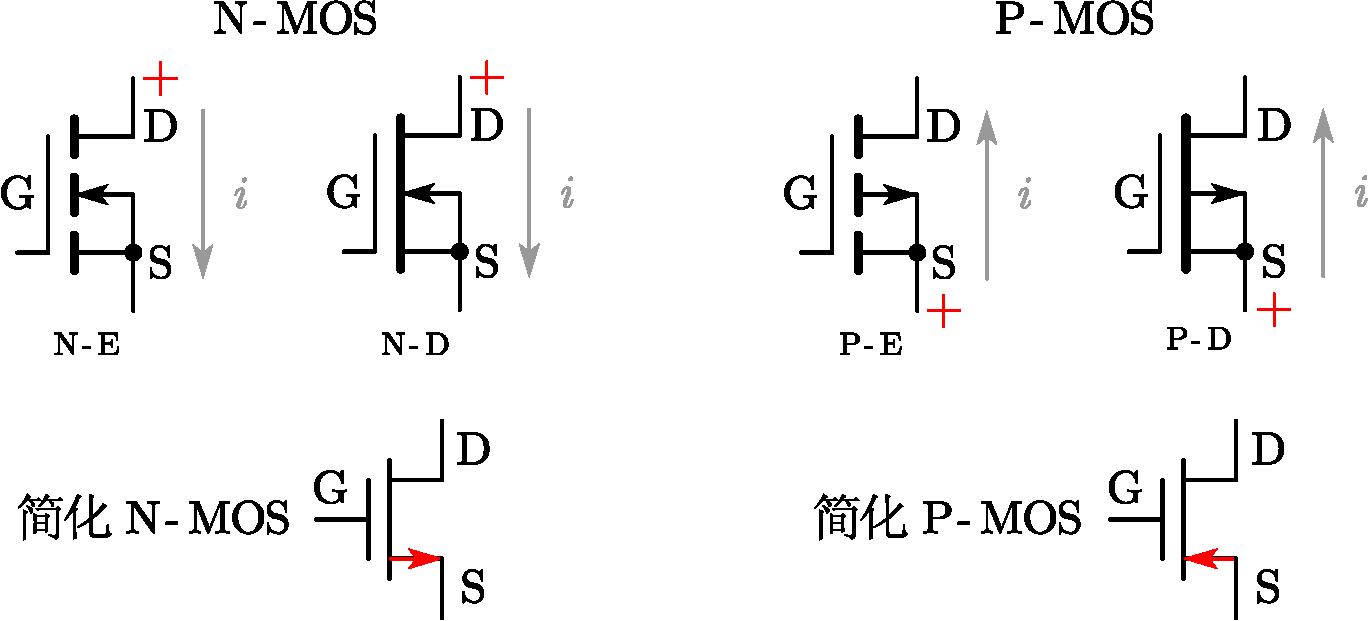
\includegraphics[width=\columnwidth]{assets/2/MOS管大全.pdf}
        \caption{ MOSFET 电路符号(ANSI 标准)与简化符号 }\label{}
    \end{figure}
\end{minipage}\end{center}



MOS 管的三个接线端分别称为栅极 G、源级 S 和漏级 D。由于 MOSFET 结构上的特点,没有电流流经栅极 G,因此可以把 D-S 看作一个二端元件,研究其伏安特性曲线 VCR。

在 N-MOS 中,栅极 G 和源级 S 之间的电压 $u_{\text{GS}}$ 会对 VCR 产生影响,主要表现为 D-S 开路(称为截止区)或非开路。在非开路情况下($u_{\text{GS}}$ 超过阈值电压),$u_{\text{DS}}$ 会影响通过的电流 $i_{\text{DS}}$。而 P-MOS 则相反,栅极 G 和漏级 D 之间的电压 $u_{\text{GD}}$ 会对 VCR 产生影响,在非开路情况下($u_{\text{GD}} > U_T$),$u_{\text{SD}}$ 会影响通过的电流 $i_{\text{SD}}$。

总而言之,无论是 N-MOS 还是 P-MOS,它们都可视为一个非线性的 VCVS。

\subsection{N-E MOSFET 外特性}

N-Channel Enhancement-Type MOSFET 的外特性总结如下:
\begin{enumerate}
\item 阈值电压 $U_T$: 使得 D-S 之间不再开路的电压阈值称为阈值电压(典型值为 1 V),需要注意 
\item 绝缘性:栅极 G 与其它电极绝缘,有 $i_{\text{GS}} = i_{\text{GD}} = 0$。
\item 最大电流 $i_{\text{DS},\text{max}}$:在非开路情况下,$i_{\text{DS},\text{max}} = \frac{K}{2}(u_{\text{GS}} - U_T)^2$,其中 $K$ 为常数(典型值 1 $\mathrm{mA\cdot V^{-2}}$)。
\item 导通电阻 $R_{\text{ON}}$: 在线性区时,MOS 管在 D-S 端体现出的电阻大小,$R = \frac{2}{K(u_{\text{GS} - U_T})}$ 通常为几百欧。
\item 电流特性 $i_{\text{DS}}$: MOS 管的电流特性可采取如下模型\footnote{模型的推导详见参考文献 \cite{电路原理导学导教} Page 30.}
\begin{equation}
i_{\text{DS}} = 
\begin{cases}
    0 &, u_{\text{GS}} < U_T \\
    K \left[ (u_{\text{GS}} - U_T)\cdot u_{\text{DS}} - \frac{u_{\text{DS}}^2}{2} \right] &, u_{\text{GS}} \geq U_T\ \& \ u_{\text{DS}} < u_{\text{GS}} - U_T \\ 
    \frac{K}{2}(u_{\text{GS}} - U_T)^2 &, u_{\text{GS}} \geq U_T\ \& \ u_{\text{DS}} \geqslant u_{\text{GS}} - U_T \\ 
\end{cases}
\end{equation}
\end{enumerate}




例如,$U_T = 1$ V,$K = 1\ \mathrm{mA \cdot V^{-2}}$ 时,N 沟道增强型 MOSFET 的电流特性如图 \ref{MOS 管的 iDS 电流特性}\footnote{Matlab 源码见附录 \ref{MOS 管的 iDS 电流特性 源码}} 所示。

\begin{figure}[H]\centering
\begin{subfigure}[t]{0.67\textwidth}\centering
    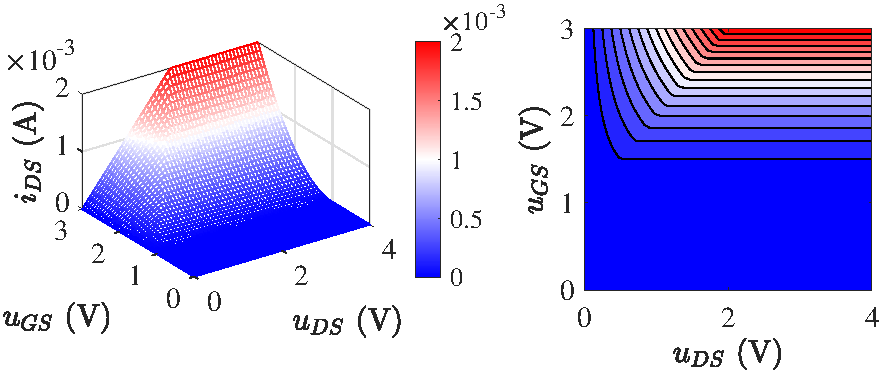
\includegraphics[height=135pt]{assets/2/MOS管外特性.pdf}
    \caption{ $i_{\text{DS}} = i_{\text{DS}}(u_{\text{DS}}, u_{GS})$ 的函数图像 }
\end{subfigure}\begin{subfigure}[t]{0.33\textwidth}\centering
    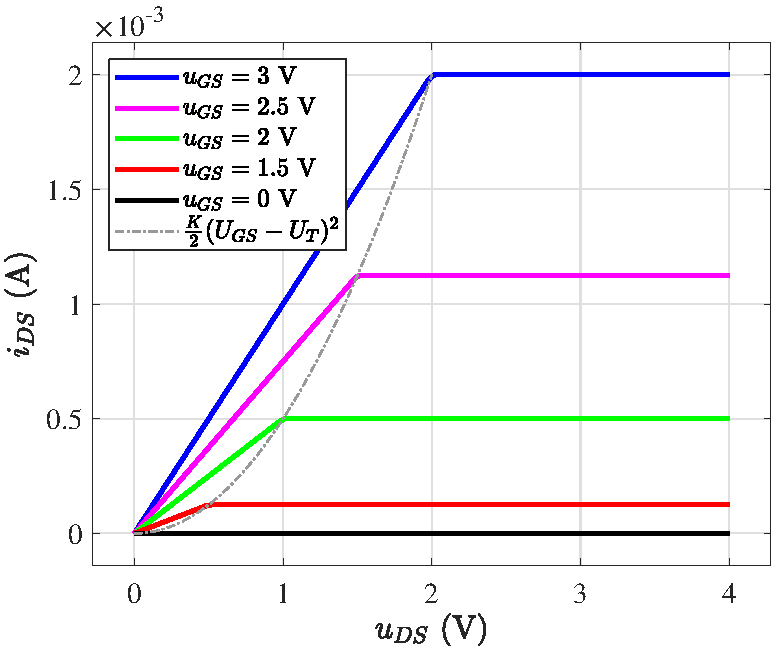
\includegraphics[height=135pt]{assets/2/MOS管外特性 (2).pdf}
    \caption{ 在给定 $U_{GS}$ 下 $i_{\text{DS}} = i_{\text{DS}}(u_{\text{DS}})$ 的函数图像 }
\end{subfigure}
\caption{ N 沟道增强型 MOSFET 的 $i_{\text{DS}}$ 电流特性 }\label{MOS 管的 iDS 电流特性}
\end{figure}

\subsection{MOSFET 等效电路}

依 MOS 管的外特性,可分为三个区,截止区、线性区和恒流区,分别对应三个等效电路,如下图所示:
\begin{figure}[H]\centering
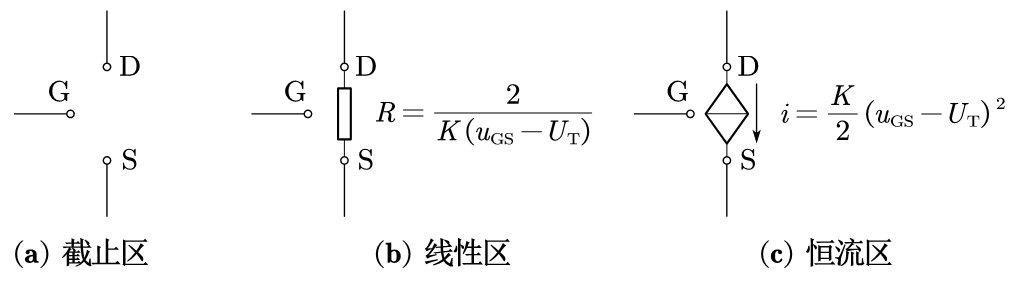
\includegraphics[width=0.63\textwidth]{assets/2/MOS管等效电路.png}
\caption{ MOS 管等效电路}\label{MOS管等效电路}
\end{figure}

事实上,MOS 管上下端连接负载(例如灯泡)时,在上方连接和在下方连接会有不同的效果,具体例子详见 \href{https://www.zhihu.com/question/34634572/answer/3421289786}{知乎: 为什么一般用 P-MOS 做上管,N-MOS 做下管}。

\section{数字系统}

\subsection{数字化的必要性}
数字化就是离散化:时间离散化和数值离散化。离散化可视为一定形式的特征提取,将一定范围内的信号值集总为一个值。数字化后,信号处理变得丰富多彩,且极大的削弱了噪声的影响。除了无法实现放大、振荡等少数信号处理方法,滤波、变频、调制解调都可以通过数字电路实现。数据压缩、解编码等在模拟系统中难以实现的信号变化功能在数字系统中很容易实现。

但也有一些场合不适合或无法数字化,例如放大器、振荡器、ADC 和 DAC 模拟端的滤波器、高频信号数字化成本高、信息处理量极大等情况。

\subsection{信号的离散化}

\subsubsection{多数位量化:}
最简单的量化是离散为 1 位数字信号(1 个二进制位),即划定电压分界值,电压信号大于此值时取 1,否则取 0。一般情况下,我们将电压范围 $[u_{\text{min}},\ u_{\text{max}}]$ 离散为 $2^n$ 个数值(即划分为 $2^n$ 个区间),共 $(2^n + 1)$ 个分界值,类似 linspace($u_{\text{min}}$, $u_{\text{max}}$, $2^n+1$),最终得到数字信号 $0, 1, 2, \cdots, 2^n - 1$。

\subsubsection{并行传输与串行传输:}
为了传递 $n$ 位的数字信号,最常见的方法是 $n$ 条线并行传输,每一个时钟周期传输 $n$ 个二进制位,等价于一个模拟信号的离散值;也可以使用串行传输,每 $n$ 个时钟周期传输 $n$ 个二进制位,等价于一个模拟信号的离散值。并行传输的通信速率远远大于串行传输,但在高频系统中,并行信号线之间的串扰问题比较严重。

\subsubsection{量化单位 $\Delta$: }
量化单位指等距离散后两相邻离散值的距离,记为 $\Delta$,$1\  \Delta = 1\  \text{LSB} =  \frac{u_{\text{max}} - u_{\text{min}}}{2^n}$。当 $u_{\text{min}} = 0$ 时,也是离散值为 1 的信号对应的电压值。量化单位越小,量化误差越小,最大量化误差为 $\frac{\Delta }{2}$。

例如,将 $[0,\ 5\ \mathrm{V}]$ 的模拟信号离散为 3 位数字信号(3 个二进制位),此时 $1\  \Delta = 0.625\ \mathrm{V}$,最大量化误差为 0.3125 V。


\section{门电路}

将模拟信号转为数字信号,并对数字信号进行传递、分析、处理,最后进行输出(可能还需要将数字信号转回模拟信号),是现代信号处理的基本流程。逻辑门是此过程的基本元件。最常用的逻辑门如图 \ref{逻辑门} (a) 所示,其中反相器、与非门、或非门是基本门,可由 MOS 管直接构成,其它门则由基本门组合而成。它们之间的关系如图 \ref{逻辑门} (b) 所示。


反相器、与门、或门、与非门、或非门、异或门、同或门的英文简写分别为 NOT、AND、OR、NAND、NOR、XOR、XNOR。

\begin{figure}[H]\centering
\begin{subfigure}[t]{0.7\columnwidth}\centering
    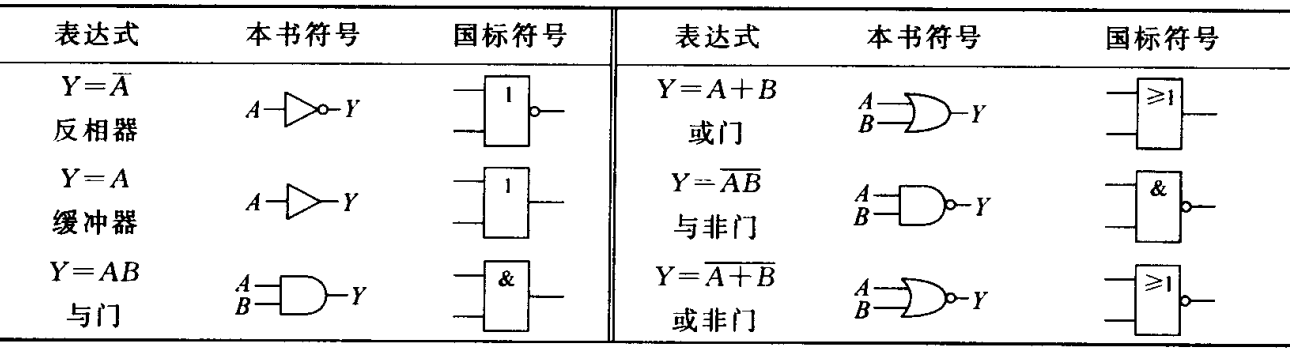
\includegraphics[height=90pt]{assets/2/逻辑门.png}
    \caption{ 几种常见的逻辑门 }
\end{subfigure}\hfill
\begin{subfigure}[t]{0.3\columnwidth}\centering
    \includesvg[height=90pt]{assets/2/逻辑门关系.drawio.svg}
    \caption{ 逻辑门之间的关系 }
\end{subfigure}
\caption{ 逻辑门 }\label{逻辑门}
\end{figure}

\subsection{数字信号的运算}

数字信号是在有限域 $\Z_2$ 上进行运算的,有两种基本二元运算,一种基本一元运算,分别是与 “$+$”、或 “$\cdot$”、非 “$-$”。两种基本二元运算具有以下性质:

\begin{enumerate}
\item 交换律:$A + B = B + A$,$A \cdot B = B \cdot A$
\item 结合律:$(A + B) + C = A + (B + C)$,$(A \cdot B) \cdot C = A \cdot (B \cdot C)$
\item 分配律:$A \cdot (B + C) = A \cdot B + A \cdot C$,${\color{red} A + B \cdot C = (A + B) \cdot (A + C)}$
\item 吸收律:$A + A \cdot B = A$
\end{enumerate}

运算非“$-$” 的性质如下:
\begin{equation}
\begin{aligned}
    &\overline{(A + B)} = \overline{A} \cdot \overline{B} ,\quad &&\overline{(A \cdot B)} = \overline{A} + \overline{B} \\
    &A + B = \overline{(\overline{A} \cdot \overline{B})},\quad && A \cdot B = \overline{(\overline{A} + \overline{B})}
\end{aligned}
\end{equation}

在基本运算的基础上,还定义了二元运算异或“$\oplus$”、同或“$\odot$”,其定义如下:
\begin{equation}
\begin{aligned}
    A \oplus B &= A \cdot \overline{B} + \overline{A} \cdot B = (A + B) \cdot (\overline{A} + \overline{B})\\
    A \odot B &= A \cdot B  + \overline{A} \cdot \overline{B} = (A + \overline{B}) \cdot (\overline{A} + B)
\end{aligned}
\end{equation}
可以证明异或“$\oplus$”、同或“$\odot$”也满足交换律、结合律以及分配率。

\subsection{基本逻辑门}\label{基本逻辑门}

可以用 N-E-MOS(N 沟道增强型 MOS 管,N-Channel Enhancement-Type MOSFET)、电源、电阻构成三种基本逻辑门,如图 \ref{由 N-MOS 构成三种基本逻辑门},但是它们的静态功率不为零。现实中广泛应用的是由 CMOS (Complementary Metal-Oxide-Semiconductor Transistor) 构成的基本逻辑门,如图 \ref{由 C-MOS 构成三种基本逻辑门} 所示,其中蓝色指 N-MOS,红色指 P-MOS。在这些基本门的结构上,相应地增加 MOS 管串联、并联的数量,可以实现 $n$ 输入的基本逻辑门。

CMOS 由一个 N-MOS 和一个 PMOS 构成,无论输入是 0 或 1,都是一个 MOS 管导通,另一个截止(断开),因此静态功率为 0。实际生产中,CMOS 是单独的一个元件,内部已经集成了 N-MOS 和 PMOS。

%\begin{figure}[H]\centering
%\begin{subfigure}[t]{0.33\columnwidth}\centering
%    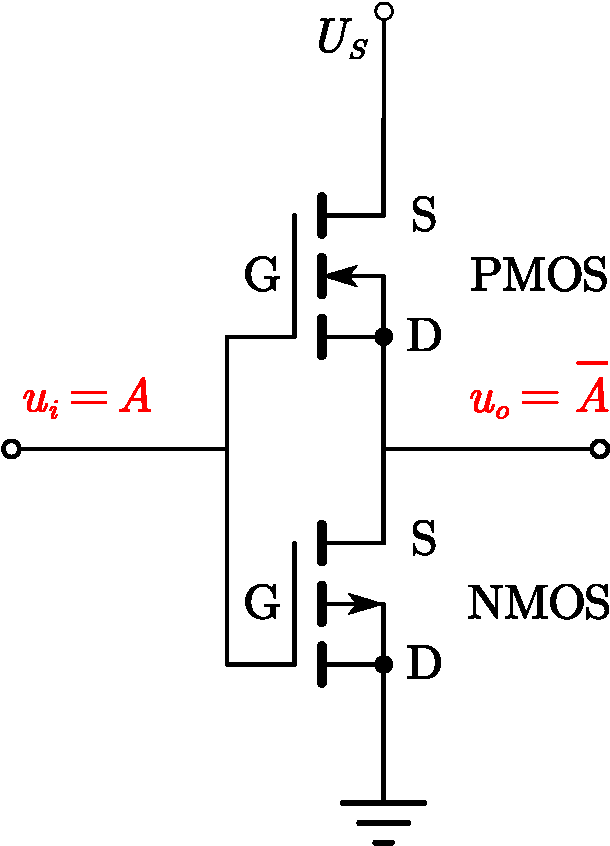
\includegraphics[height=125pt]{assets/2/反相器.pdf}
%    \caption{ 反相器(CMOS) }
%\end{subfigure}\hfill
%\begin{subfigure}[t]{0.33\columnwidth}\centering
%    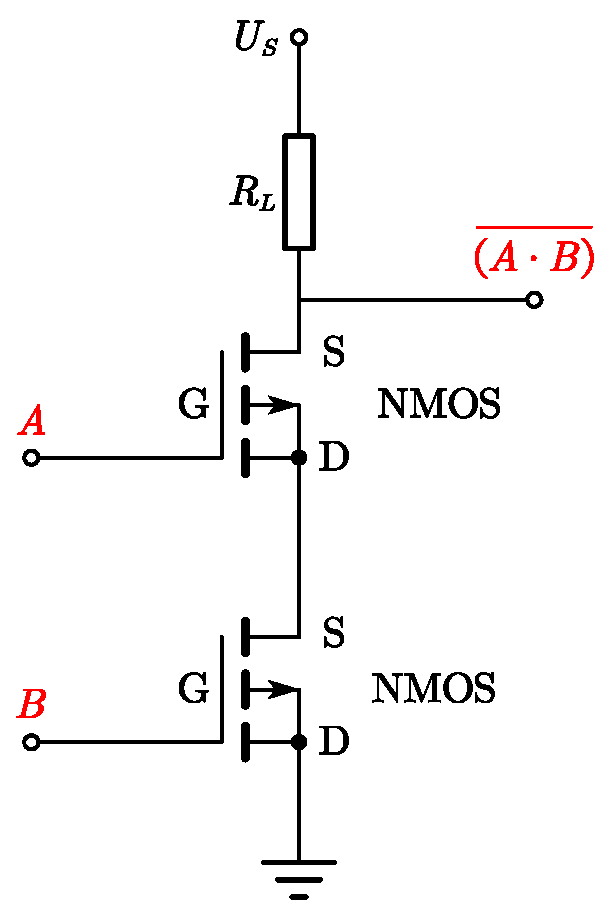
\includegraphics[height=125pt]{assets/2/与非门.pdf}
%    \caption{ 与非门 }
%\end{subfigure}
%\begin{subfigure}[t]{0.33\columnwidth}\centering
%    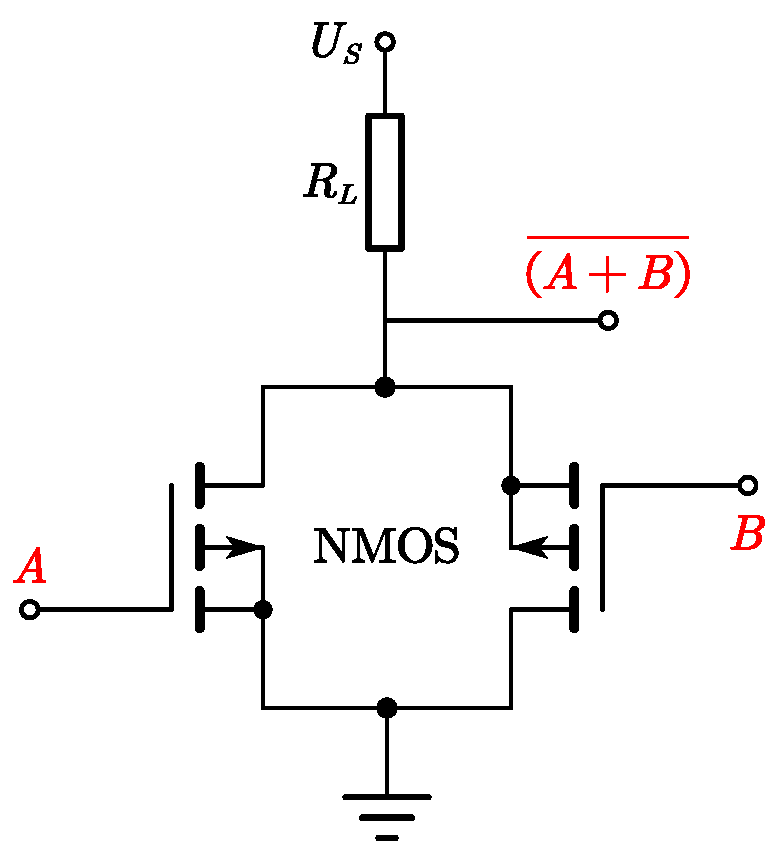
\includegraphics[height=125pt]{assets/2/或非门.pdf}
%    \caption{ 或非门 }
%\end{subfigure}
%\caption{ 基本逻辑门 }\label{基本逻辑门}
%\end{figure}

\begin{figure}[H]\centering
\begin{subfigure}[t]{0.33\columnwidth}\centering
    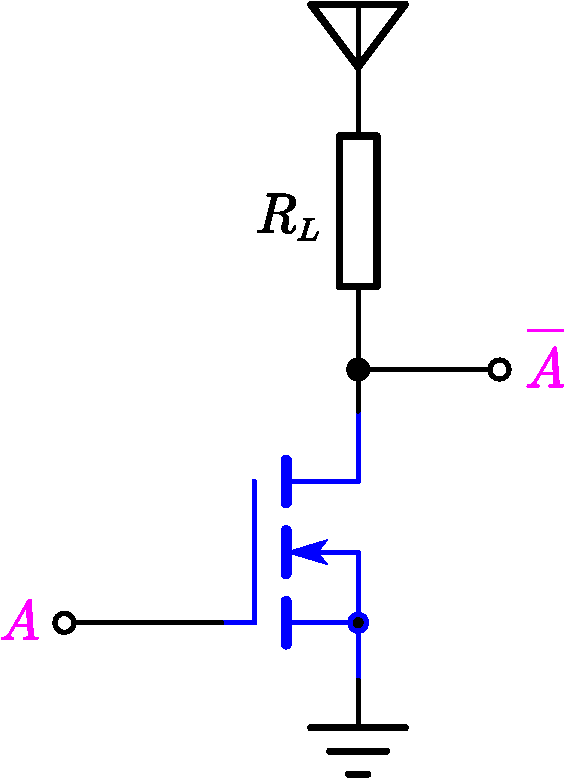
\includegraphics[height=120pt]{assets/2/NMOS NOT.pdf}
    \caption{ N-MOS NOT }
\end{subfigure}\hfill
\begin{subfigure}[t]{0.33\columnwidth}\centering
    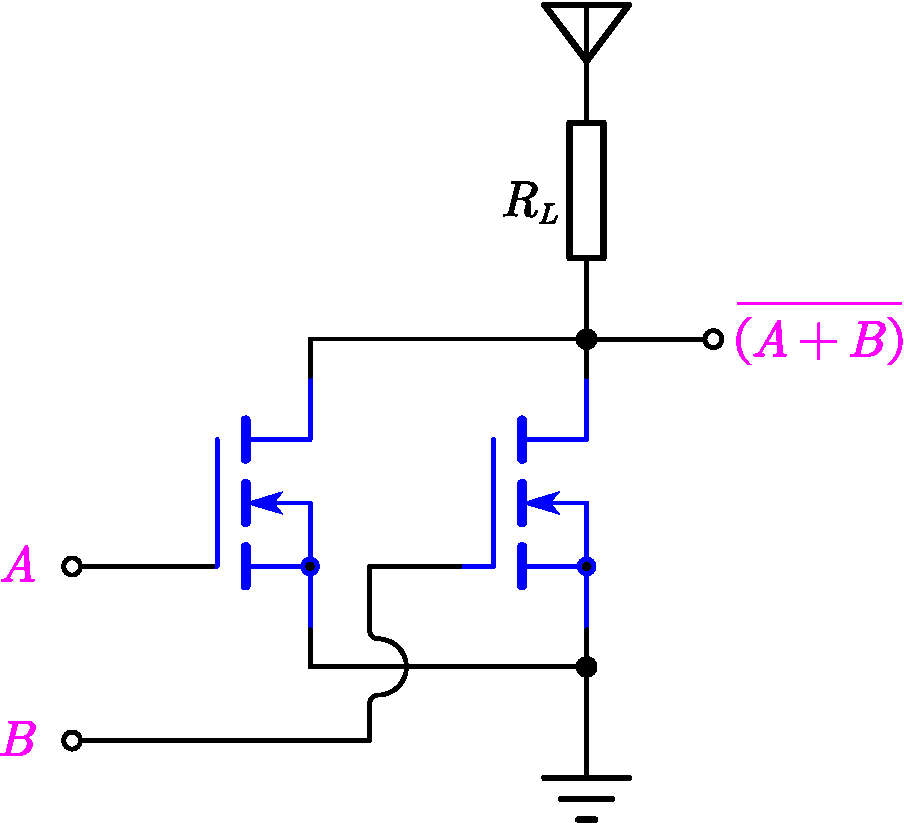
\includegraphics[height=120pt]{assets/2/NMOS NOR.pdf}
    \caption{ N-MOS NOR }
\end{subfigure}
\begin{subfigure}[t]{0.33\columnwidth}\centering
    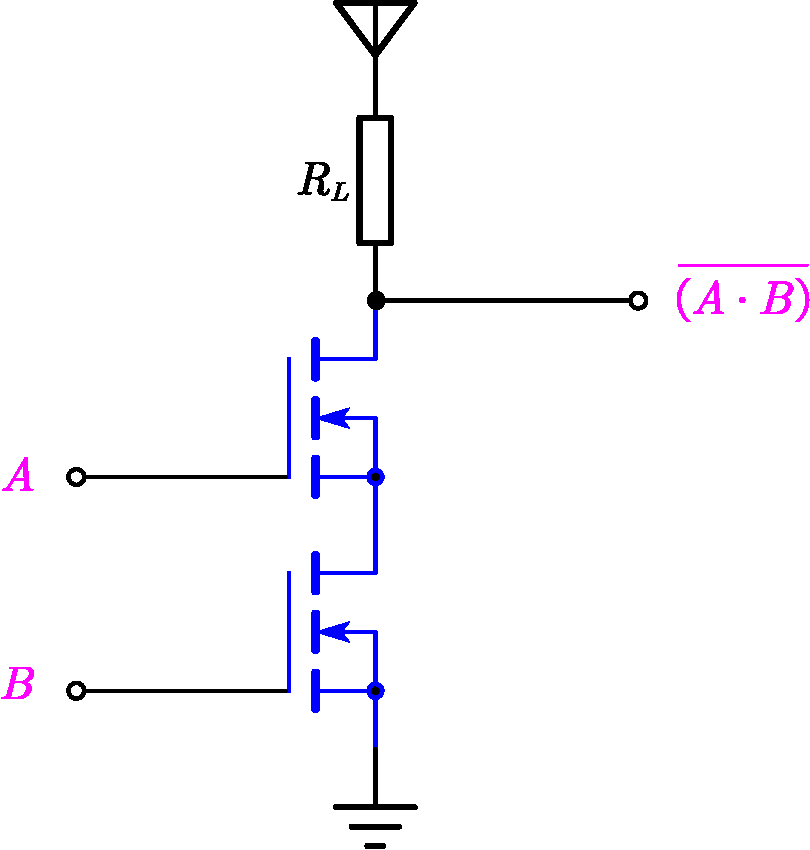
\includegraphics[height=120pt]{assets/2/NMOS NAND.pdf}
    \caption{ N-MOS NAND }
\end{subfigure}
\caption{ 由 N-MOS 构成三种基本逻辑门 }\label{由 N-MOS 构成三种基本逻辑门}
\end{figure}

\begin{figure}[H]\centering
    \begin{subfigure}[t]{0.33\columnwidth}\centering
        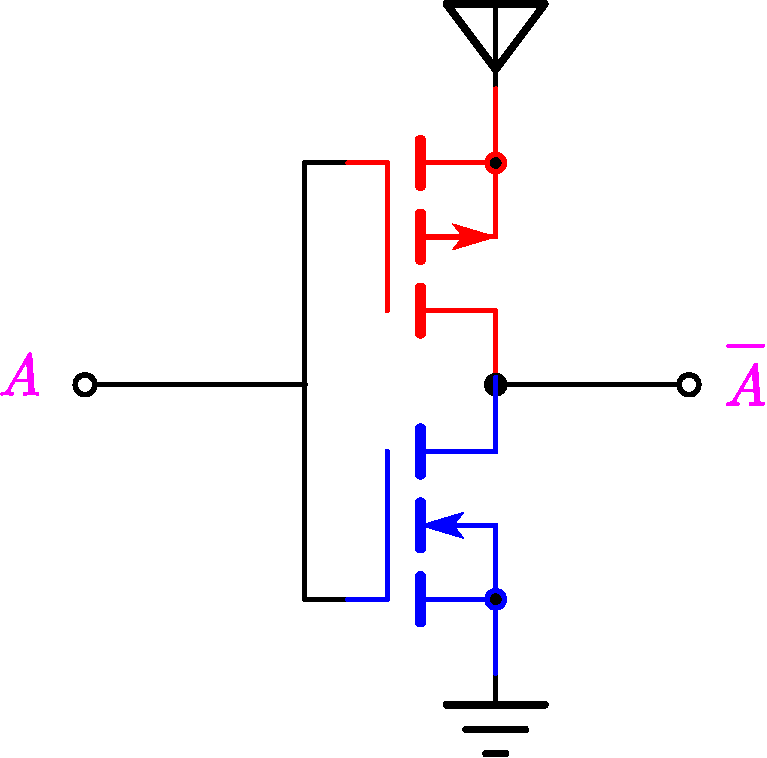
\includegraphics[height=120pt]{assets/2/CMOS NOT.pdf}
        \caption{ C-MOS NOT }
    \end{subfigure}\hfill
    \begin{subfigure}[t]{0.33\columnwidth}\centering
        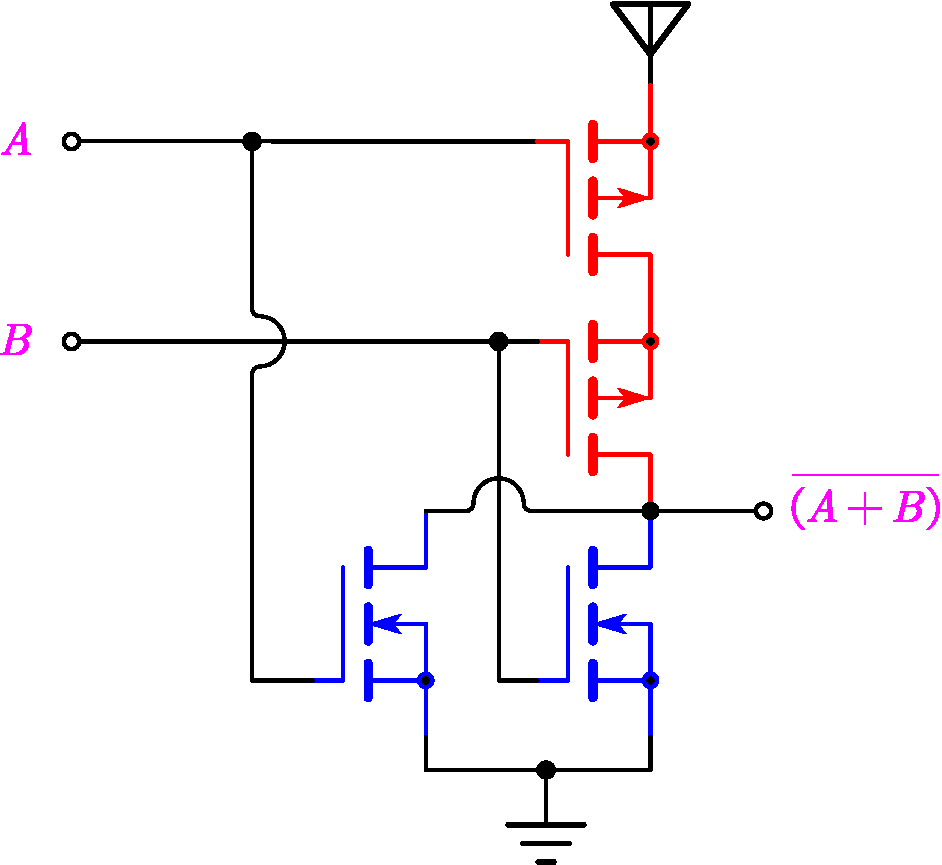
\includegraphics[height=120pt]{assets/2/CMOS NOR.pdf}
        \caption{ C-MOS NOR }
    \end{subfigure}
    \begin{subfigure}[t]{0.33\columnwidth}\centering
        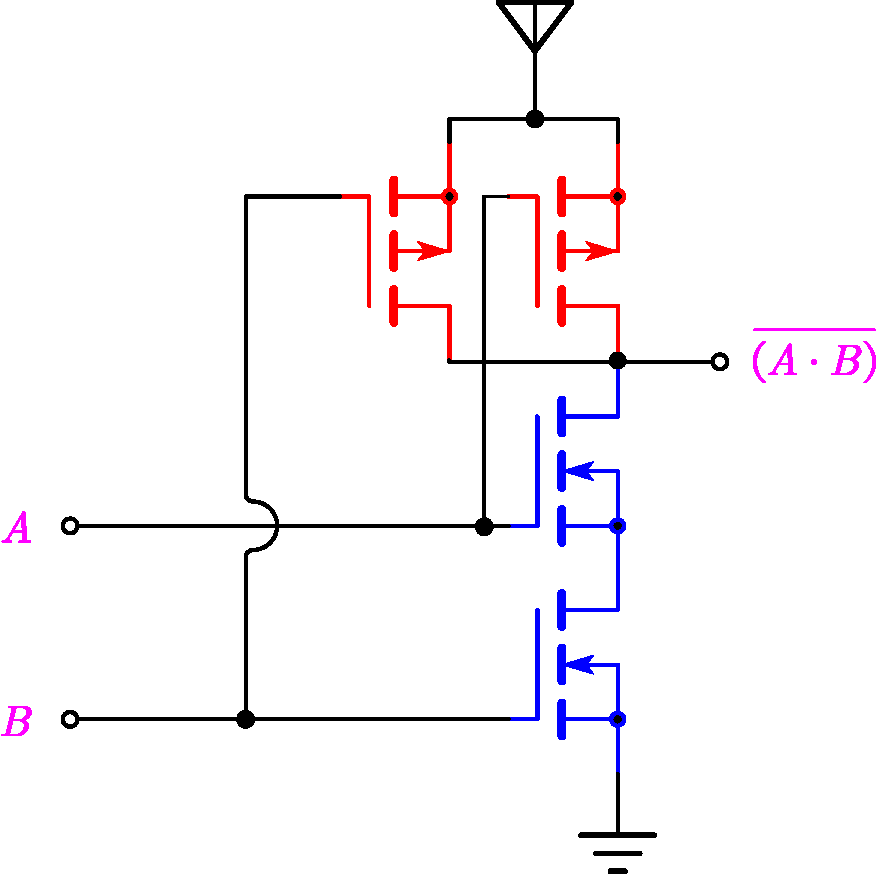
\includegraphics[height=120pt]{assets/2/CMOS NAND.pdf}
        \caption{ C-MOS NAND }
    \end{subfigure}
    \caption{ 由 C-MOS 构成三种基本逻辑门 }\label{由 C-MOS 构成三种基本逻辑门}
\end{figure}

为了方便参考,我们再给出 CMOS XOR 的电路图,如图 \ref{CMOS XOR},其静态功率为 0。

\begin{figure}[H]\centering
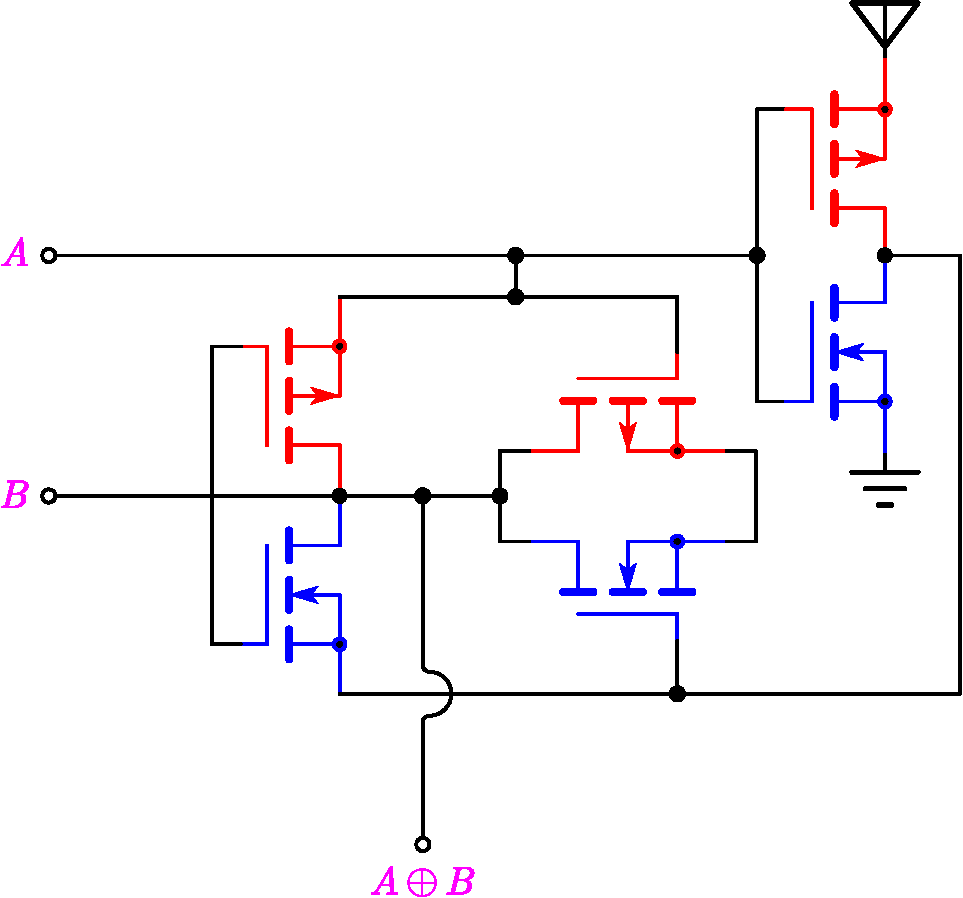
\includegraphics[width=0.42\columnwidth]{assets/2/CMOS XOR.pdf}
\caption{ CMOS XOR }\label{CMOS XOR}
\end{figure}

需要指出,上面的门电路只是几个例子,现实中实际使用的门电路可能比它们复杂得多,有时也用二极管和三极管来构成门电路,具体的例子见 \href{https://www.zhihu.com/question/36577129/answer/68096454}{知乎:怎样用电路符号表示异或门}。反相器 NOT 的功耗与其它特性可参考 \href{https://blog.csdn.net/vivid117/article/details/100083567}{数字电路基础知识:反相器(噪声容限、VTC、转换时间、速度的影响因素、传播延时等)}。

\subsection{ADC 与 DAC}


简单的 ADC、DAC 可由二极管、电阻、运算放大器构成,后者详见“第二次习题课课前练习”。

\subsection{半加器(一位加法器)}

半加器是一种基本的逻辑电路,用于将两个二进制数相加,输出一个两位的二进制数,表示相加的结果。输出的高位和低位分别称为“进位$C$”、“和位$S$”。也就是说,半加器实际上是“一位加法器”,能够处理两个一位二进制数的相加,并输出一个两位二进制结果。设输入为 $A$ 和 $B$,则有:
\begin{gather}
Y = (C S)_{(2)} = A_{(2)} + B_{(2)}
\\
C = A \cdot B,\quad S = (A + B)\cdot \overline{C} = (A + B)\cdot \overline{(A \cdot B)} = (A + B)\cdot (\overline{A} + \overline{B})  = A\cdot \overline{B}  + \overline{A}\cdot B =  A \oplus B
\end{gather}

因此构造半加器最直接的方法是用一个异或门  XOR  和 一个与门 AND(3 N+ 3 P + 3 N 共 9 个 MOS)。如果要求使用的 MOS 尽量少(仅使用 N-MOS),对逻辑表达式作处理,利用下面式子可得最简半加器电路(7 个 N-MOS)。

\begin{equation}
    C = \overline{(\overline{A\cdot B})},\quad S = \overline{\left[(A \cdot B) + \overline{(A + B)}\right]}
\end{equation}

它们的数字电路见图 \ref{半加器 HA 数字电路},实际电路见图 \ref{半加器 HA 实际电路}。

\begin{figure}[H]\centering
\begin{subfigure}[t]{0.5\columnwidth}\centering
    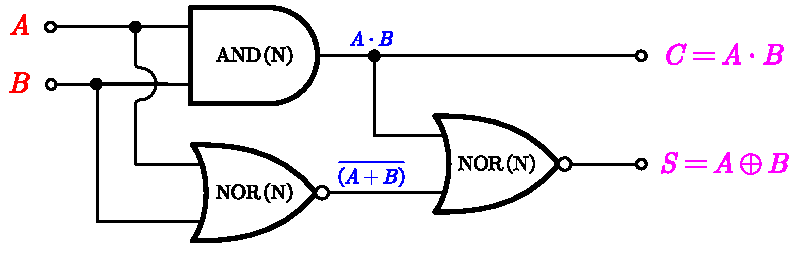
\includegraphics[height=80pt]{assets/2/NMOS 半加器数字电路.pdf}
    \caption{ N-MOS HA 数字电路}
\end{subfigure}\hfill
\begin{subfigure}[t]{0.5\columnwidth}\centering
    \includegraphics[height=80pt]{assets/2/CMOS 半加器数字电路.pdf}
    \caption{ C-MOS HA 数字电路 }
\end{subfigure}
\caption{ 半加器 HA 数字电路 }\label{半加器 HA 数字电路}
\end{figure}

\begin{figure}[H]\centering
\begin{subfigure}[t]{0.42\columnwidth}\centering
    \includegraphics[height=170pt]{assets/2/NMOS 半加器实际电路.pdf}
    \caption{ N-MOS HA 实际电路 }
\end{subfigure}\hfill
\begin{subfigure}[t]{0.58\columnwidth}\centering
    \includegraphics[height=155pt]{assets/2/CMOS 半加器实际电路.pdf}
    \caption{ C-MOS HA 实际电路 }
\end{subfigure}
\caption{ 半加器 HA 实际电路 }\label{半加器 HA 实际电路}
\end{figure}

\subsection{全加器(三输入一位加法器)}

由半加器可以进一步构造全加器,全加器是一种能够处理{\color{red} 三个一位二进制数}相加的逻辑电路,输出一个两位的二进制数 $Y= (C_o S)_{(2)}$,表示相加的结果。输出的高位称为进位 $C_o$,低位称为和位 $S$。也就是说,全加器可以理解为“三输入一位加法器”。记全加器的三个输入为 $A$,$B$,$C$,它们都是一位的二进制数,则全加器可写为:
\begin{gather}
Y= (C_oS)_{(2)} = A_{(2)} + B_{(2)} + C_{(2)} 
\\ 
C = A \cdot B + A \cdot C + B \cdot C,\quad 
S = A \oplus B \oplus C
\end{gather}


角标 $(2)$ 表示上式为二进制运算。由两个 HA 和一个 OR 即可构成全加器,数字电路如图 \ref{全加器 FA}。

\begin{figure}[H]\centering
\includegraphics[width=0.65\columnwidth]{assets/2/全加器.pdf}
\caption{ 全加器 FA}\label{全加器 FA}
\end{figure}




\subsection{四位加法器}

四位加法器,输入两个四位二进制数 $X$ 和 $Y$,分别记作 $ X= (X_3 X_2 X_1 X_0)_{(2)}$,$ Y=  (Y_3 Y_2 Y_1 Y_0)_{(2)}$,输出一个五位二进制数 $Z = (C S_3 S_2 S_1 S_0)_{(2)}$,代表两数相加的结果。原理及数字电路如图 \ref{四位加法器} 所示。

\begin{figure}[H]\centering
\includegraphics[width=0.9\columnwidth]{assets/2/四位加法器.pdf}
\caption{ 四位加法器}\label{四位加法器}
\end{figure}



\chapter{线性电阻电路分析方法}
线性电阻电路,是指仅含独立源、受控源和线性电阻的电路。$2b$ 法是利用 KCL 和 KVL 的最基本方法,对具有 $b$ 条支路 $n$ 个节点的电路,列出 $(n -1)$ 个 KCL 方程和 $(b - n +1)$ 个 KVL 方程进行求解,较为繁琐。本章将介绍多种线性电阻电路分析方法,其中几种非常重要,不仅是一种方法,更应当作一种思想,要能够熟练而灵活地运用,例如节点电压法等。


\section{支路电流法}

列出节点处的 KCL 和所有网格的 KVL 进行求解,略。

\section{节点电压法}

直接给出总结:对于含有 $n$ 个节点(内含 $p$ 个无伴电压源),$q$ 受控源控制变量的电路,在选定合适的参考点后,共列出 $n-1+q$ 个方程进行求解。其中有 $n-1$ 个节点 KCL 方程(内含 $p$ 个特殊方程,由无伴电压源直接给出,可能含超节点),$q$ 个受控限制方程,求解得到 $ n-1 $ 个电压变量(剩余一个是电压参考点)和 $q$ 个受控源变量。

\subsection{没有无伴电压源}

$p = 0$ 时,没有无伴电压源,可列出节点电压法的标准方程(设共有 $n+1$ 个节点):
\begin{equation}
    \boldsymbol{G}\cdot \vec{u} = \vec{i},\quad 
    \begin{bmatrix}
        G_{11}&G_{12}&\cdots&G_{1k}&\cdots&G_{1n}\\G_{21}&G_{22}&\cdots&G_{2k}&\cdots&G_{2n}\\\vdots&\vdots&&\vdots&&\vdots\\G_{k1}&G_{k2}&\cdots&G_{kk}&\cdots&G_{kn}\\\vdots&\vdots&&\vdots&&\vdots\\G_{n1}&G_{n2}&\cdots&G_{nk}&\cdots&G_{nn}\end{bmatrix}\begin{bmatrix}U_{1}\\U_{2}\\\vdots\\U_{k}\\\vdots\\U_{n}\end{bmatrix}=\begin{bmatrix}I_{\mathrm{Sn}, 1}\\I_{\mathrm{Sn}, 2}\\\vdots\\I_{\mathrm{Sn}, k}\\\vdots\\I_{\mathrm{Sn}, n}
    \end{bmatrix}
\end{equation}
其中,$G_{kk}$ 是第 $k$ 个独立节点的自电导,也即节点 $k$ 所有支路上的电导之和;$G_{ij}\ (i \ne j)$ 是节点 $i$ 和节点 $j$ 之间的互电导,数值上等于节点 $i$ 与节点 $j$ 间的所有电导之和并 {\color{red} 冠以负号}。特别地,节点之间仅有电流源的支路互电导为 0。$I_{\ \text{Sn,k}}$ 是第 $k$ 个节点的所有电流源电流之和(包括由有伴电压源等效而来的电流),{\color{red} 流入节点的电流取正}。

在仅含电阻、有伴电压源和电流源的电路中(没有受控源),互电导 $G_{ij} = G_{ji}$,因此电导系数矩阵 $\boldsymbol{G} = \boldsymbol{G}^T$。注意,在列节点电压法的方程时,我们记流入节点的电流为正,这是在 KCL 中假设了流出节点的电流取正得到的结果。

\subsection{一个无伴电压源}

对于仅有一个无伴电压源的情况,将参考节点选在无伴电压源的负极,仍可以列出节点电压法的标准方程,此后同上。

\subsection{多个无伴电压源}

有 $p$ 个无伴电压源时($p>1$),将参考点选在其中一个的负极(其实也可以不选),然后将剩余的无伴电压源看作超节点。列出各节点的 KCL 方程,其中,超节点的自电导由超节点中的子节点贡献(不止一项),与其它节点的互电导是整个大节点与另一节点之间的互电导。具体的例子见参考文献 \cite{电路原理} Page 108 的例 3.2.5,以及 Homework 5,这里不再赘述。


\section{回路电流法}

直接给出总结,对含有 $n$ 个网孔(内含 $p$ 个无伴电流源),$q$ 受控源控制变量的电路,使用网格电流法,共列出 $n + q$ 个方程进行求解。其中有 $n$ 个网格电压方程(内含 $p$ 个特殊方程,由无伴电流源直接给出,可能含超网格),$q$ 个受控源控制变量方程,求解得到 $n$ 个网格电流变量和 $q$ 个受控源变量。

\subsection{没有无伴电流源}

$p=0$ 即没有无伴电流源时,可列出回路电流法的标准方程\footnote{在本文,回路电流法一律使用网格电流变量,因此“回路电流法”和“网格电流法是同一含义。”}: 

\begin{equation}
    \boldsymbol{R}\cdot \vec{i} = \vec{u},\quad 
    \begin{bmatrix}
        R_{11}&R_{12}&\cdots&R_{1k}&\cdots&R_{1n}\\R_{21}&R_{22}&\cdots&R_{2k}&\cdots&R_{2n}\\\vdots&\vdots&&\vdots&&\vdots\\R_{k1}&R_{k2}&\cdots&R_{kk}&\cdots&R_{kn}\\\vdots&\vdots&&\vdots&&\vdots\\R_{n1}&R_{n2}&\cdots&R_{nk}&\cdots&R_{nn}\end{bmatrix}\begin{bmatrix}I_{1}\\I_{2}\\\vdots\\I_{k}\\\vdots\\I_{n}\end{bmatrix}=\begin{bmatrix}U_{\text{sn},1}\\U_{\text{sn},2}\\\vdots\\U_{\text{sn},k}\\\vdots\\U_{\text{sn},n}
    \end{bmatrix}
\end{equation}

其中,$R_{kk}$ 为第 $k$ 个网孔的自电阻,即网孔上的所有电阻之和;$R_{ij}\ (i\ne j)$ 是第 $i$ 个网孔与第 $j$ 个网孔的互电阻,也即两个网孔重合部分的所有电阻之和并 {\color{red} 冠以负号}。特别地,网孔之间仅有电压源时互电阻为 0,网孔没有重合部分(不相邻)时,互电阻也为 0。$U_{\text{sn,} k}$ 是第 $k$ 个网孔中所有电压源的电压升之和(包括由有伴电流源等效而来的电压),{\color{red} 沿网孔电流方向的电压取正}。

在仅含线性电阻、有伴电压源和电流源的电路中(没有受控源),互电阻 $R_{ij} = R_{ji}$,因此电阻系数矩阵 $\boldsymbol{R} = \boldsymbol{R}^T$。需要注意,网格回路电流是假想出来的,实际电流是它们的叠加(背后由叠加定理支撑)。

\subsection{含有无伴电流源}

有 $p$ 个无伴电流源时($p \geqslant 1$),将与电流源相邻的网格合并,看作超网格。列出超网格的 KVL 方程时,超网格的自电阻仍由内部的子网格贡献(不止一项),与其它网格的互电阻是整个超网格与另一网格的互电阻。如果含有无伴电流源,且仅属于一个网格(无法构成超网格),则此网格的 KVL 方程写为电流源方程即可,其它不变(例如 Homework 5.8)。

具体的例子见参考文献 \cite{电路原理} Page 115 的例 3.3.5,以及 Homework 5,这里不再赘述。



\section{叠加、齐性、替代定理}

\subsection{叠加定理与齐性定理}

由线性元件和独立电源组成的电路称为线性电路。无论是选用电流作为变量,还是选用电压作为变量列出电路方程,最终得到都是线性方程组。而线性方程组的解具有可加性(additivity property)和齐次性(homogeneity property),反映到电路中即为响应和激励(独立电源)之间满足可加性和齐次性,称前者为叠加性质(superposition property),称后者为比例性质。

从线性代数的角度来看,假设 $\vec{x}_1$ 和 $\vec{x}_2$ 都是线性方程组 $\boldsymbol{A} \cdot \vec{x} = \vec{b}$ 的解,那么 $\vec{x}_3 = \vec{x}_1 + \vec{x}_2$ 是方程组的解,这对应了叠加定理,并且 $\forall\ k \in \R,\ \vec{x}_4 = k\cdot \vec{x}_1$ 也是方程组的解,这对应了齐性定理。


\begin{LineTheorem}[叠加定理,Superposition Theorem]\label{叠加定理}
    在一个具有唯一解的线性电阻电路中,所有激励(独立电源)共同作用时产生的响应(电压和电流),等于各激励单独作用时产生的响应之和(代数和)。电压源不作用时成短路,电流源不作用时成开路。特别地,如果电路中含有受控源,它应保留在电路中,被控量与控制量之间的关系保持不变,但控制量随着激励的不同而改变。
\end{LineTheorem}

\begin{LineTheorem}[齐性定理,Homogeneous Theorem]\label{齐性定理}
对于一个具有唯一解的线性电子电路,当电路中所有的激励(独立电源)都变化 $k$ 倍,那么电路中的响应(电压和电流)也都变化 $k$ 倍。
\end{LineTheorem}

注意,不能直接用叠加定理或齐性定理求解功率(功率为 2 次方,非线性),应先求出电压或电流,得到叠加后的结果,再计算功率。


\subsection{替代定理}

替代定理是对电路等效变换的一种方法,它用电压源或电流源来等效替代某条支路或部分电路,替代前后电路中各支路电压电流不发生变化。替代定理的应用较为广泛,它适用于任意电路。

\begin{LineTheorem}[替代定理,Substitution Theorem]\label{替代定理}
    对任意电路,假设电路中某条支路两端的电压为 $U$,流经该支路的电流为 $I$。则该支路既可以用一个电压为 $U$ 的独立电压源替代,也可以用一个电流为 $I$ 的独立电流源替代。其中,电压源的极性与原支路电压极性相同,电流源的方向与原支路电流方向相同,替代后电路中各支路电压电流与替代前电路中相应的变量相等。
\end{LineTheorem}

需要强调,替代定理作的是“替代”而不是“等效”。前者是在此工作点上的替代,而后者是对外 $u$-$i$ 关系的等效。一旦电路中各支路电压电流发生变化,替代定理就不再适用。此外,还需要被替代的支路与电路中其它支路之间无耦合关系。

\section{戴维南定理和诺顿定理}

\begin{LineTheorem}[戴维南定理,Thevenin's Theorem]\label{戴维南定理}
    所有的一端口线性电阻电路对外都可以等效为一个理想电压源 $U$ 和电阻 $T$ 串联。电压源 $U$ 等于端口处的开路电压 (Open-circuit Voltage),电阻 $R$ 是该端口内部所有{\color{red} 独立电源}(受控源仍保留)不起作用(又称“置零”)时端口处的等效电阻。
\end{LineTheorem}

\begin{LineTheorem}[诺顿定理,Norton's Theorem]\label{诺顿定理}
    所有的一端口线性电阻电路对外都可以等效为一个理想电流源 $I$ 和一个电导 $G$ 并联。电流源 $I$ 等于端口处的短路电流 (Short-circuit Current),电导 $G$ 是该端口内部所有{\color{red} 独立电源}(受控源仍保留)不起作用(又称“置零”)时端口处的等效电导。
\end{LineTheorem}

“置零”即将电压源移去后两端短路,将电流源移去后两端开路。

\section{特勒根定理}


\begin{BlockTheorem}[特勒根定理,Tellegen's Theorem\footnote{又称为特勒根定理似功率守恒定理 (Tellegen's Quasi-power Theorem)}]\label{特勒根定理}
    若电路 $N$ 和 $\hat{N}$ 具有相同的拓扑结构\footnote{称两个电路具有相同的拓扑结构如果它们具有相同的支路数、节点数,且支路和节点联接关系也相同。},则所有支路中的电压与对方对应支路电流的乘积之和为零,即:
    \begin{equation}
    \sum u_k \cdot \hat{i}_k = u_1\hat{i}_1 + u_2\hat{i}_2 + \cdots + u_n\hat{i}_n = 0,\quad 
    \sum \hat{u}_k \cdot i_k = \hat{u}_1 i_1 + \hat{u}_2 i_2 + \cdots + \hat{u}_n i_n = 0
    \end{equation}
\end{BlockTheorem}
特勒根定理是由基尔霍夫定律直接导出的,因此适用于任意电路。特别地,作为常见的情况,对{\color{red} 纯电阻网络}(不要求电阻线性)有:

将给定电路的支路(共 $b$ 支)分为外部($1 \sim b_0$)和内部支路($b_0 + 1 \sim b$),则特勒根定理可表示为:
\begin{equation}
\sum_{k=1}^{b_0} u_k \cdot \hat{i}_k + \boxed{\sum_{k=b_0+1}^{b} u_k \cdot \hat{i}_k} = 0
,\quad 
\sum_{k=1}^{b_0} \hat{u}_k \cdot i_k + \boxed{\sum_{k=b_0+1}^{b} \hat{u}_k \cdot i_k} = 0
\end{equation}
方框圈出的部分是内部项,只有在证明了这两项相等时(例如 {\color{red} 内部网络是纯电阻电路}),才可得到常用结论:
\begin{equation}
\sum_{k=1}^{b_0} u_k \cdot \hat{i}_k = \sum_{k=1}^{b_0} \hat{u}_k \cdot i_k
\end{equation}


\section{互易定理}

互易定理共有三种形式,分别对应了纯线性电阻二端口的 $\boldsymbol{G}$ 参数互易、$\boldsymbol{R}$ 参数互易和 $\boldsymbol{H}$ 参数互易,分别对应 $\boldsymbol{R} = \boldsymbol{R}^T$,$\boldsymbol{G} = \boldsymbol{G}^T$ 和 $H_{12} + H_{21} = 0$。特别注意,互易定理仅适用于 {\color{red} 只含线性电阻的二端口},也即纯线性电阻二端口。


\begin{BlockTheorem}[互易定理 Ⅰ]\label{互易定理 Ⅰ}
对任意一个仅含线性电阻的二端口,在 11' 端口接入电压激励 $u_{s1}$ 时得到 22' 端口的短路电流为 $i_2$,在 22' 端口接入电压激励 $u_{s2}$ 时得到 11' 端口的短路电流为 $i_1$,则有:
\begin{equation}
\frac{i_2}{u_{s1}} = \frac{i_1}{u_{s2}} \Longleftrightarrow u_1 i_{1} = u_2 i_{2}
\end{equation}
特别地,当 $u_{s1} = u_{s2}$ 时,有 $i_2 = i_1$,即交换两端口激励位置,得到的响应电流不变。
\end{BlockTheorem}

\begin{BlockTheorem}[互易定理 Ⅱ]\label{互易定理 Ⅱ}
对任意一个仅含线性电阻的二端口,在 11' 端口接入电流激励 $i_{s1}$ 时得到 22' 端口的开路电压为 $u_2$,在 22' 端口接入电流激励 $i_{s2}$ 时得到 11' 端口的开路电压为 $u_1$,则有:
\begin{equation}
\frac{u_2}{i_{s1}} = \frac{u_1}{i_{s2}} \Longleftrightarrow u_{1} i_1 = u_{2} i_2
\end{equation}
特别地,当 $i_{s1} = i_{s2}$ 时,有 $u_2 = u_1$,即交换两端口激励位置,得到的响应电压不变。
\end{BlockTheorem}

\begin{BlockTheorem}[互易定理 Ⅲ]\label{互易定理 Ⅲ}
    对任意一个仅含线性电阻的二端口,在 11' 端口接入电流激励 $i_{s1}$ 时得到 22' 端口的开路电压为 $u_2$,在 22' 端口接入电压激励 $u_{s2}$ 时得到 11' 端口的短路电流为 $i_1$,则有:
    \begin{equation}
        \frac{i_{s1}}{i_2} = \frac{u_{s2}}{u_{1}} \Longleftrightarrow u_{1} i_1 = u_{2} i_2
    \end{equation}
\end{BlockTheorem}

总的来讲,无论是哪种形式,当激励为电流源时,另一端响应是开路电压;当激励为电压源时,另一端响应为短路电流。并且总有 $u_1i_1 = u_2 i_2$。需要特别注意的是,在 Ⅰ、Ⅱ 两种情况,只要统一规定了正方向(例如电流向上为正,电压上正下负),则总有 $u_1i_1 = u_2 i_2$ 成立。而在情况 Ⅲ,两个电流的 {\color{red} 正方向必须相反},这体现在 $H_{12} = - H_{21}$ 的负号上。


\section{对偶电路和对偶原理}

\section{定理适用范围总结}


在下表中,“任意电路”指可非线性、非时变电路;“线性电路”指仅含线性元件(包括但不限于线性电阻、线性受控源)和独立源的电路;“线性电阻电路”指仅含线性电阻、线性受控源和独立源的电路;“纯电阻网络”指仅含电阻的网络,电阻可非线性;“纯线性电阻二端口”指仅含线性电阻的二端口。

\begin{table}[H]\centering
    %\renewcommand{\arraystretch}{1.5} % 调整行间距为 1.5 倍
    %\setlength{\tabcolsep}{1.5mm} % 调整列间距
    \caption{定理适用范围总结}
    \label{定理适用范围总结}
\begin{tabular}{cccccccccc}\toprule
    定理 & 范围  \\
    \midrule
    节点电压法、回路电流法 &线性电阻电路 \\
    替代定理 & 任意电路 \\
    叠加定理、齐性定理 & 线性电路 \\
    戴维南定理、诺顿定理 & 线性电阻电路\\
    特勒根定理 & 任意电路 \\
    特勒根定理应用 & {\color{red} 纯电阻网络} \\
    互易定理 & 线性电路 \\
    互易定理的应用 & {\color{red} 纯线性电阻二端口} \\
    对偶原理 &  \\
    \bottomrule
\end{tabular}
\end{table}



\chapter{非线性电阻电路分析}\thispagestyle{fancy}

\section{非线性电阻电路}

非线性电阻电路,是指电路中含有非线性电阻元件的电路。


\subsection{非线性电阻}

线性电阻(linear resistance)的阻值 $R = \frac{u}{i} = \tan \alpha = \text{\ const}$ 为定值,非线性电阻(nonlinear resistance)的阻值会随电压或电流发生变化,可表示为如下形式: 
\begin{center}\noindent\begin{minipage}{0.49\columnwidth}
    \begin{gather}
        \text{流控型:} u = u(i) \\ 
        \text{压控型:} i = i(u)
    \end{gather}
\end{minipage}\hfill\begin{minipage}{0.49\columnwidth}
    \begin{figure}[H]\centering
    %\includegraphics[width=0.4\columnwidth]{}
    \caption{非线性电阻的符号}\label{非线性电阻的符号}
    \end{figure}
\end{minipage}\end{center}

需要注意,非线性电阻电路的 $u$-$i$ 关系不满足齐次性和可加性,因此叠加定理不再适用。


\subsection{几种常见的二极管}

整流二极管\footnote{后文所说的“二极管”,如无特别说明,都是指整流二极管}、稳压二极管和发光二极管是最常用的非线性电阻,它们的伏安特性曲线类似(参数不同),正常工作时:
\begin{gather}
i = i(u) = I_\text{S}\left(e^{\frac{u}{U_{\text{TH}}}} - 1\right)
\end{gather}
其中,$U_{\text{TH}}$ 为常数,典型值 $25 \mV$(注意不是导通电压 $U_{\text{sd}}$);$I_\text{s}$ 称为反相饱和电流(硅二极管典型值为 $10^{-12} \ \mathrm{A}$)\footnote{有关二极管或其他元件的详细参数,可到\href{https://www.szlcsc.com/}{立创商城}进行检索并查看数据手册 (date sheet),例如典型二极管 \href{https://item.szlcsc.com/65968.html}{SM4007PL} 的数据手册在 \href{https://atta.szlcsc.com/upload/public/pdf/source/20240710/496933BE705816864AC9581E766E463F.pdf}{here}。}。

另外,还有隧道、充气二极管等。隧道二极管是一种压控型非线性电阻,在 $u-i$ 图中($u$ 是横坐标),伏安特性形似字母 N,因此也称为 N 型非线性电阻;充气二极管是一种流控型非线性电阻,也称为 S 型非线性电阻。

\begin{figure}[H]\centering
\begin{subfigure}[t]{0.52\columnwidth}\centering
    \includegraphics[height=135pt]{assets/4/常见二极管.pdf}
    \caption{ 常见二极管的电路符号 }
\end{subfigure}\hfill
\begin{subfigure}[t]{0.48\columnwidth}\centering
    \includegraphics[height=140pt]{assets/4/整流二极管.png}
    \caption{ 整流二极管的伏安特性曲线 }
\end{subfigure}
\caption{二极管的符号与伏安特性}
\end{figure}

\subsection{非线性电阻电路解的唯一性条件}

如果一个非线性电阻的 $u$-$i$ 曲线上任意的(不同)两点 $(u_1, i_1)$,$(u_2, i_2)$ 都满足:
\begin{equation}
(u_2 - u_1) \cdot (i_2 - i_1) > 0
\end{equation}
则称此电阻为严格递增电阻。非线性电阻电路存在唯一解的一个充分条件就是:\footnote{详见参考文献 \cite{电路原理} Page 158}
\begin{enumerate}
\item 每个电阻都是严格递增电阻
\item 每个电阻都满足 $\displaystyle \lim_{u \to \infty}  i = \infty$
\item 电路中不存在仅由独立电压源构成的回路或仅由独立电流源联接的两个支点
\end{enumerate}

\section{非线性电阻电路的求解}

\subsection{四种常见解法}
\begin{enumerate}
\item 方程法(解析法):

当电路是直流,且工作点确定的时候,电路有确定的唯一解,可以使用方程法。列出电路的代数方程(组),利用 Matlab 等计算软件求解非线性方程(组)的解,即得最终结果。在列写代数方程组时,仍可以沿用节点电压法的思路(列出电流 KCL),或者回路电流法的思路(列出电压 KVL),详见参考文献 \cite{电路原理} Page 159 的例 4.2.3 和例 4.2.4。

\item 图解法:

图解法可用于大致估计电路的解,这在非线性元件有多个工作区时(例如二极管)有奇效,但不适用于求解精确解。详见参考文献 \cite{电路原理} Page 160,这里不多赘述。

\item 分段线性法:

将非线性电阻的伏安曲线分段线性化,从而使非线性电路转化为线性电路,然后便可等效为线性电子电路进行求解。\footnote{分段线性法可能导致电路有多解或无解,这超出了本课程的范围,本书始终假设运用分段线性法时,非线性电阻电路存在唯一解。}此方法还需要确定电阻的工作区(即哪一个线性段),先排除明显不可能的范围,再用假设法来验证即可。

\item 小信号法:
小信号法是指,如果非线性电阻的激励由直流和交流两部分构成,且交流的幅值比较小,则在其工作点附近,可用线性电阻来近似此非线性电阻。

小信号法常用于求解存在小扰动(例如小幅交流信号)的直流激励非线性电路时,这是实际中经常遇到的情况,不过它对存在大扰动的电路则无能为力。
\end{enumerate}

现实中求解电路时,常常将上面几种方法相结合,混合使用。

\subsection{二极管的四种近似模型}
在分段线性法的指导下,我们可以提处二极管的四种常见近似模型:

\begin{gather}
\begin{cases}
    i = 0                                &, u < U_{\text{sd}} \\ 
    i = \frac{u - U_{\text{sd}}}{R} &, u > U_{\text{sd}} \\
\end{cases}\quad 
\begin{cases}
    i = 0 &, u < U_{\text{sd}} \\ 
    u = U_{\text{sd}} &, i > 0 \\
\end{cases}\quad 
\begin{cases}
    i = 0 &, u < 0 \\ 
    i = \frac{u}{R} &, u > 0 \\
\end{cases}\quad 
\begin{cases}
    i = 0 &, u < 0 \\ 
    u = 0 &, i > 0 \\
\end{cases}
\end{gather}
\begin{figure}[H]\centering
\includegraphics[width=\columnwidth]{assets/4/二极管的四种近似模型.pdf}
\caption{二极管的四种近似模型}\label{二极管的四种近似模型}
\end{figure}
其中,模型 4 也称为理想二极管模型。从左往右,模型的近似程度越大,分析起来也越简单。-

\subsection{小信号法}
假设非线性电阻的工作点为 $(U_0, I_0)$,且在此工作点附近可近似为线性电阻,则对电流 $i = i(u)$ 或电压 $u = u(i)$,在工作点 $(U_0, I_0)$ 处作泰勒展开:
\begin{gather}
i = i(U_0) + \left(\frac{\mathrm{d} i}{\mathrm{d} u }\right)_{u=U_0}(u - U_0) = I_0 + G_d\cdot \Delta u = I_0 + \Delta i
,\quad 
G_d = 
\left.\begin{matrix}\displaystyle
    \frac{\mathrm{d} i}{\mathrm{d} u }
\end{matrix}\right|_{u=U_0}
\\
u = u(I_0) + \left(\frac{\mathrm{d} u}{\mathrm{d} i }\right)_{i=I_0}(i - I_0) = U_0 + R_d \cdot \Delta i = U_0 + \Delta u
,\quad 
R_d =
\left.\begin{matrix}\displaystyle
    \frac{\mathrm{d} u}{\mathrm{d} i }
\end{matrix}\right|_{i=I_0}
\end{gather}
其中 $G_d$、$R_d$ 是元件在工作点处的线性近似,分别称为动态电导(Dynamic Conductance)和动态电阻(Dynamic Resistance),需要注意它们是工作点处的切线斜率(或其倒数)而非原点与工作点构成的割线斜率(割线是静态电导/电阻)。

需要注意,小信号法看似与叠加定理相似,实际上是两种不同的思路,考虑的是激励的微小变化给响应带来的影响,而叠加定理是考虑不同激励的叠加。
\section{用 MOSFET 构成放大器(略)}

\section{非线性电阻应用举例(略)}
\subsection{整流}
\subsection{限幅}
\subsection{倍频}


\chapter{动态电路的时域分析}\thispagestyle{fancy}

\section{电容和电感}
电容:
\begin{gather}
q = Cu
\Longrightarrow 
\begin{cases}
    i = C \frac{\mathrm{d} u }{\mathrm{d} t } \\ 
    u = \frac{1}{C} \int i \mathrm{d} t
\end{cases},\quad E_C = \frac{1}{2}Cu^2 \\ 
\text{串联:} \frac{1}{C} = \sum \frac{1}{C_i},\quad \text{并联:}C = \sum C_i
\end{gather}

电感:
\begin{gather}
    \Phi = L i
    \Longrightarrow 
    \begin{cases}
        u = L \frac{\mathrm{d} i }{\mathrm{d} t } \\ 
        i = \frac{1}{L} \int u \mathrm{d} t
    \end{cases},\quad E_L = \frac{1}{2}Li^2\\ 
    \text{串联:} L = \sum L_i,\quad \text{并联:}\frac{1}{L} = \sum \frac{1}{L_i}
\end{gather}

\begin{figure}[H]\centering
\begin{subfigure}[b]{0.21\columnwidth}\centering
    \includegraphics[width=\columnwidth]{assets/5/电容.png}\
    \vspace*{3mm}
    \caption{电容}
\end{subfigure}
\begin{subfigure}[b]{0.21\columnwidth}\centering
    \includegraphics[width=\columnwidth]{assets/5/实际电容.png}
    \caption{实际电容}
\end{subfigure}\hfill
\begin{subfigure}[b]{0.21\columnwidth}\centering
    \includegraphics[width=\columnwidth]{assets/5/电感.png}
    \vspace*{3mm}
    \caption{电感}
\end{subfigure}
\begin{subfigure}[b]{0.21\columnwidth}\centering
    \includegraphics[width=\columnwidth]{assets/5/实际电感.png}
    \caption{实际电感}
\end{subfigure}
\caption{电容和电感的符号}
\end{figure}


\begin{center}
\noindent\begin{minipage}{0.49\columnwidth}
    \hspace*{2em} 由于电容、电感和电阻等无源元件通常较大,在电路中占据更多的空间,因此集成电路设计中会尽量少用这些元件。

    \hspace*{2em} MOSFET 的 G、D、S 各极之间都存在寄生电容,这些电容通常是 $u_{GS}$ 和 $u_{DS}$ 的函数,并且还会随温度变化,其中影响最大的是 $C_{GS}$。本书我们主要讨论 $C_{GS}$,并且认为其是恒定值。
    
    MOSFET 的 SRC (Switch-Resistor-Capacitor) 模型如右图所示。我们将在后文“反相器的输出延迟”一例中讨论寄生电阻所带来的影响。当然,也可以有 SSC (Switch-Source-Capacitor) 模型,这里不多赘述。
\end{minipage}\hfill\begin{minipage}{0.4\columnwidth}
\begin{figure}[H]\centering
\includegraphics[height=150pt]{assets/5/MOSFET SRC模型.png}
\caption{MOSFET 的 SRC 模型}\label{MOSFET SRC模型}
\end{figure}
\end{minipage}\end{center}

\section{换路定理}
动态电路中电路结构或参数变化引起的电路变化统称为“换路” (Switch)。假设电路在 $t = 0$ 时刻发生换路,把换路前一瞬间记为 $t = 0^-$,换路后一瞬间记为 $t = 0^+$,则微分方程的初始条件就是各参数在 $t = 0^+$ 时的值,称为初始值。

依据电容和电感的定义,有界函数积分所得到的函数是连续的,因此有下面的换路定律。
\begin{BlockTheorem}[换路定律]\label{换路定律}
对任意电容,如果在换路瞬间电容电流为有限值,则有:
\begin{equation}
u_{C}(0^+) = u_{C}(0^-),\quad q_{C}(0^+) = q_{C}(0^-)
\end{equation}
对任意电感,如果在换路瞬间电感电压为有限值,则有:
\begin{equation}
i_{L}(0^+) = i_{L}(0^-),\quad \Phi_{L}(0^+) = \Phi_{L}(0^-)
\end{equation}
\end{BlockTheorem}

需要强调的是,当两个电容串联时,换路定律不再适用,因为这时两电容中间的电流可以是无穷大。

\section{一阶动态电路}

用一阶常微分方程来描述的电路称为“一阶动态电路”,简称为一阶电路 (First Order Circuit)。只含有一个动态元件(电容或电感)的电路一定是一阶电路,含有多个电容(或多个电感)的电路也可能是一阶电路。
如果一阶电路中只含有一个动态元件,则可以把该动态元件以外的电路用戴维南定理进行等效,从而得到经典的串联 $RC$ 电路或串联 $RL$ 电路。

我们称激励恒为 0 (对 $t>0$) 的解为“零输入响应”,称电容(电感)初始能量为 0 的解为“零状态响应”。


\subsection{一阶线性微分方程}

对一阶线性微分方程:
\begin{equation}
y' + p(x)y = q(x)
\end{equation}
考虑它的齐次方程 $y' + p(x)y = 0$,得到齐次解 $y_h$ : 
\begin{equation}
    y_h = y(0) e^{-\int_{0}^{x}p(x)\,\mathrm{d}x}
\end{equation}
再求出原方程的一个特解 $y_p$,则方程的通解为 $y = y_p + y_h = y_p(x) + y(0) e^{-\int_{0}^{x}p(x)\,\mathrm{d}x}$。特别地,当 $p(x)$ 和 $q(x)$ 都为常量时,一个特解是 $y \equiv \frac{q}{p}$,此时的通解为:
\begin{equation}
y = \frac{q}{p} + y(0)e^{-px}
\end{equation}

为了方便参考,用因子法给出一个普适的通解形式。在原方程两边同乘因子 $\mu(x) = e^{\int_{0}^{x}p(x)\mathrm{d}x}$,此时 $\mu'(x) = p\, e^{\int_{0}^{x}p \mathrm{d}x} = p \mu$,且 $\mu(0) = 0$,于是有:
\begin{gather}
\mathrm{d} \left(\mu y \right) = q\mu\ \mathrm{d}x
\Longrightarrow 
\left[\mu y\right]_0^x = \int_{0}^{x} q \mu \mathrm{d}x \\ 
\Longrightarrow y = y(x) = \frac{1}{\mu} \int_{0}^{x} q \mu\ \mathrm{d}x 
\end{gather}

\subsection{经典解法}

经典法求解一阶电路,便是根据 KCL 和 KVL 以及元件特性列写电路的微分方程(组),然后求解微分方程(组)的解。

考虑常见的串联 $RC$ 电路,设激励 $U_s$ 恒定不变,则换路之后有:
\begin{equation}
u_C = u_C(t) = U_s + \left[u_C(0^+) - U_s\right] e^{-\frac{t}{\tau}} = u_C(0^+)e^{-\frac{t}{\tau}} + U_s\left[1 - e^{-\frac{t}{\tau}}\right],\quad \tau = RC
\end{equation}
我们称 $U_s$ 项为稳态分量(或强制分量),它是 $t \to \infty$ 时电路的响应;称 $\left(u_C(0^+) - U_s\right) e^{-\frac{t}{\tau}}$ 一项为自由分量,它是电容状态发生变化所带来的响应。$\tau$ 称为“时间常量”,它决定了电路的响应速度,$\tau$ 越小,电路响应越快。一般认为经过 $3\tau \sim 5 \tau$ 的时间,电路响应便达到稳态。

类似地,对串联 $RL$ 电路,则有:
\begin{equation}
i_L = i_L(t) = \frac{U_s}{R} + \left[i_L(0^+) - \frac{U_s}{R}\right]e^{-\frac{t}{\tau}} = i_L(0^+)e^{-\frac{t}{\tau}} + \frac{U_s}{R}\left[1 - e^{-\frac{t}{\tau}}\right],\quad \tau = \frac{L}{R}
\end{equation}
其中 $u_C(0^+)$ 和 $i_L(0^+)$ 是初始条件,也常记为 $u_{C,0^+}$ 和 $i_{L,0^+}$。

\subsection{三要素法}
设 $f = f(t)$ 是某支路的待求参量(可以是电压或电流),定义 $f_{\infty}(t) = f(t)\mid_{t \to \infty}$ 是 $t \to \infty$(稳态)时 $f(t)$ 的表达式。那么,参数的通解是:
\begin{equation}
\boxed{
    f = f(t) = f_{0^+}\cdot e^{-\frac{t}{\tau}} + \left[ f_{\infty}(t) - f_{\infty}(0)\cdot e^{-\frac{t}{\tau}} \right] = \left[f_{0^+} - f_{\infty}(0)\right]\cdot e^{-\frac{t}{\tau}} + f_{\infty}(t)
}\quad 
\text{三要素}
\begin{cases}
    f_{0^+} \\ 
    f_{\infty} \\ 
    \tau
\end{cases}
\end{equation}
特别地,当 $f_{\infty}$ 为常量时,$f_{\infty}(0) \equiv f_{\infty}(t)$,有:
\begin{equation}
\boxed{
    f = f(t) = f_{0^+}\cdot e^{-\frac{t}{\tau}} + f_{\infty}(0)\cdot \left[ 1 - e^{-\frac{t}{\tau}} \right]
}
\end{equation}
只要确定了三要素,便能够确定方程的解。作为一个例子,考虑激励为 $U_s = U_m \sin (\omega t + \phi)$ 的一阶串联 $RL$ 电路,现在来求解 $i_L = i_L(t)$。电感 $L$ 的阻抗为 $\omega L$,可以得到电流的稳态解 $i_{L,\infty}$ :\footnote{我们将在下一章讨论这样做的正确性}
\begin{equation}
i_{L, \infty} = \frac{U_m}{\sqrt{R^2 + (\omega L)^2}} \sin \left(\omega t + \phi - \varphi \right),\quad \varphi =  \arctan \frac{\omega L}{R} > 0
\end{equation}
时间常量 $\tau = \frac{L}{R}$,记电感的初始电流 $i_{L,0^+} = I_0 $(原始储能为 $E = \frac{1}{2}LI_0^2$),便可以得到:
\begin{align}
i_L(t) &= i_{L,0^+} \cdot e^{-\frac{t}{\tau}} + i_{L, \infty}(t) -  i_{L, \infty}(0)\cdot e^{-\frac{t}{\tau}} \\
&= \left[i_{L,0^+} - i_{L, \infty}(0)\right] \cdot e^{-\frac{t}{\tau}} + i_{L, \infty}(t)\\
&= 
\left[I_0 - \frac{U_m}{\sqrt{R^2 + (\omega L)^2}} \sin \left(\phi - \varphi \right) \right] \cdot e^{-\frac{t}{\tau}}
+ \frac{U_m}{\sqrt{R^2 + (\omega L)^2}} \sin \left(\omega t + \phi - \varphi \right)
\end{align}
式中前一项为自由分量,后一项为稳态分量。

在第六章介绍“相量法”之后,这类方程的求解将变得简单。

\section{一阶动态电路应用}
RC 微分积分电路、OPA 微分积分电路、滤波全桥整流 (AC > DC) 等部分详见参考文献 \cite{电路原理} Page 207-223,我们不多赘述。下面介绍一些结论性的内容。


\subsection{反相器的传播延迟 (NOT Gate)}

图 \ref{} 是由两个 N-MOS 反相器构成的缓冲器,受 MOSFET 寄生电阻的影响(主要是 $C_{\text{GS}}$),输入与输出数字信号间的存在延迟,称为“传播延迟” (Propagation Delay)。过程详见参考文献 \cite{电路原理} Page 207-223\footnote{注意,这里我们给出的结论与参考文献 \cite{电路原理} 不同,后者的结论是有些问题的。},我们直接给出结论:
\begin{gather}
    t_\text{pd, $0\to 1$} = \left(R_{\text{ON, 1}} \parallel R_{\text{D, 1}}\right) C_{\text{GS, 2}}\cdot \ln \left(\frac{V_{\text{H}} - V_{\text{L}}}{{\color{red} V_{\text{0}, \min}} - V_{\text{L}}}\right)
    ,\quad 
    t_\text{pd, $1\to 0$} = R_{\text{D, 1}} C_{\text{GS, 2}}\cdot \ln \left(\frac{V_{\text{H}} - V_{\text{L}}}{V_{\text{H}} - {\color{red} V_{\text{0}, \max}}}\right)
\end{gather}

\noindent 式中各参数意义如下:
\begin{enumerate}
\item $V_\text{L}$ : 反相器稳定时的输出低电压,即输入稳定在 1 时输出的逻辑 0 低电压;
\item $V_\text{H}$ : 反相器稳定时的输出高电压,即输入稳定在 0 时输出的逻辑 1 高电压;
\item $V_{0,\min}$ : $V_{0,\min} = u_{\text{GS}}|_{u_{\text{o}} = V_{\text{OH}, \min}}$ 是反相器输出电压为 $V_{\text{OH},\min}$ 时的 GS 间电压,即使得反相器输出 $u_{\text{o}} = V_{\text{OH},\min}$ 时的输入电压 $u_{\text{GS}}$,它由反相器的 $u_i$-$u_o$ 特性和电压协议中的 $V_{\text{OH},\min}$ 共同确定
\item $V_{0,\max}$ : 类似地,$V_{0,\max} =  u_{\text{GS}}|_{u_{\text{o}} = V_{\text{OL}, \max}}$ 是反相器输出电压为 $V_{\text{OL},\max}$ 时的 GS 间电压,它是由反相器的 $u_i$-$u_o$ 特性和电压协议中的 $V_{\text{OL},\max}$ 共同确定。
\end{enumerate}

\begin{figure}[H]\centering
    \includegraphics[width=0.8\columnwidth]{assets/5/反相器的传播延迟.png}
    \caption{由两个 N-MOS 构成的反相器}\label{N-MOS 反相器}
\end{figure}

%对 $V_{\text{IH}}$,应将其理解为高电平输入的临界值 Minimum Input High Voltage $V_{\text{IH}, \min}$,对反相器来说,当 $u_i > V_{\text{IH}}$ 时,输出电压 $u_o$ 为低电平(认为是瞬间完成变化);类似,对 $V_{\text{IL}}$,应将其理解为低电平输入的临界值 Maximum Input Low Voltage $V_{\text{IL}, \max}$,对反相器而言,当 $u_i < V_{\text{IL}}$ 时,输出电压 $u_o$ 为高电平(认为是瞬间完成变化)。并且,实际中使用的元件都有 $V_{\text{OH}} > V_{\text{IH}} > V_{\text{IL}} > V_{\text{OL}}$。

作为一个精度还不错的近似(也是最常见的情况),我们认为两个反相器的参数完全相同,令 $V_{\text{L}} = 0$、$V_{\text{H}} = V_{\text{DD}}$,作近似 $V_{0,\min} \approx V_{\text{T}}$($V_{\text{T}}$ 是 MOS 的阈值电压,2N7000 的典型值为 2 V),并且 $R_{\text{D}} \gg R_{\text{ON}} \Longrightarrow R_{\text{ON}} \parallel R_{\text{D}} \approx R_{\text{ON}}$。此时有:
\begin{gather}
    t_\text{pd, $0\to 1$} = R_{\text{ON}} C_{\text{GS}}\cdot 
    \ln \left(\frac{V_{\text{DD}}}{V_\text{T}}\right) \quad 
    t_\text{pd, $1\to 0$} = R_{\text{D}} C_{\text{GS}}\cdot \ln \left(\frac{V_{\text{DD}}}{V_{\text{DD}} - V_\text{T}}\right)
\end{gather}
代入各项数据的典型值,我们可以得到一个大致的传播延迟。
\begin{gather}
V_{\text{DD}} = 5 \ \mathrm{V},\quad V_\text{T} = 2 \ \mathrm{V} ,\quad R_{\text{ON, 1}} = 5 \ \Omega,\quad C_{\text{GS}} = 10 \ \mathrm{pF} \\ 
t_\text{pd, $0\to 1$} = 5 \ \Omega\times 10 \pF \times \ln \left(\frac{5 \ \mathrm{V}}{2 \ \mathrm{V}}\right) = 0.046 \ \mathrm{ns}  \\
t_\text{pd, $0\to 1$} = 1 \kO\times 10 \pF \times \ln \left(\frac{5 \ \mathrm{V}}{5 \ \mathrm{V} - 2 \ \mathrm{V}}\right) = 5.108 \ \mathrm{ns}
\end{gather}


%通常情况下,四个电压参数的测量是简单的。还是以反相器为例,设地电压 $V_\text{SS} = 0$ 而电路电源为 $V_{\text{DD}} = 5 \ \mathrm{V}$,且四个电压参数都在 $[V_{\text{SS}}, V_{\text{DD}}]$ 之间。测量方法如下:
%\begin{enumerate}
%\item $V_{\text{IH}}$ : 将输入逻辑从 0 缓慢增至 1(即输入电压从 $V_{\text{SS}}$ 缓慢增加到 $V_{\text{DD}}$),反相器的输出电压会在某点 $v_i = v_{i1}$ 开始下降,然后在很近的一点 $v_i = v_{i2} > v_{i1}$ 处停止下降。通常可取 $V_{\text{IH}} = \frac{v_{i1} + v_{i2}}{2}$ 或者 $V_{\text{IH}} = v_{i2}$。
%\item $V_{\text{IL}}$ :  将输入逻辑从 1 缓慢减至 0(即输入电压从 $V_{\text{DD}}$ 缓慢减小到 $V_{\text{SS}}$),反相器的输出电压会在某点 $v_i = v_{i2}$ 开始上升,然后在很近的一点 $v_i = v_{i1} < v_{i2}$ 处停止下降。通常可取 $V_{\text{IL}} = \frac{v_{i1} + v_{i2}}{2}$ 或者 $V_{\text{IH}} = v_{i1}$。
%\item $V_{\text{OH}}$ : 在输入电压下降至 $v_i < V_{\text{IL}}$ 的区间中,$v_o$ 的稳定值即为 $V_{\text{OH}}$,例如 $v_i = V_{\text{SS}}$ 时的输出电压。
%\item $V_{\text{OH}}$ : 在输入电压上升至 $v_i > V_{\text{IH}}$ 的区间中,$v_o$ 的稳定值即为 $V_{\text{OL}}$,例如 $v_i = V_{\text{DD}}$ 时的输出电压。
%\end{enumerate}

\subsection{脉冲序列发生器 (OPA 正反馈)}
\subsection{三角波发生器 (脉冲序列下的 RC 电路)}
\subsection{降压斩波电路 (Buck)}

\section{二阶动态电路}
\section{二阶线性常系数微分方程}
二阶线性微分方程如下:
\begin{equation}
y'' + p(x)y' + q(x)y = f(x)
\end{equation}
它的求解并不容易,我们本课仅限于常系数的情况,即 $p(x) = p$ 和 $q(x) = q$ 为常数,通常写成衰减系数 $\beta$ 和固有频率 $\omega_0$ 的形式:
\begin{equation}
y'' + 2\beta y' + \omega_0 y = f(x)
\end{equation}
考虑它的齐次解 $y_h$,我们直接给出结论:
\begin{gather}
\begin{aligned}
    &\text{欠阻尼:} &&\beta < \omega_0, &&y(t) = e^{-\beta t} A\sin \left( \omega t + \phi \right) \\ 
    &\text{临界阻尼:} &&\beta = \omega_0, &&y(t) = e^{-\beta t} (A + Bt) \\
    &\text{过阻尼:} &&\beta > \omega_0, &&y(t) = e^{-\beta t}\left( A\,e^{\omega t} + B\,e^{-\omega t}\right)
\end{aligned}
\end{gather}
设其稳态解(特解)为\textbf{常数} $y_s$(非常数的情况在下一章会谈),在电路中即为 $y_\infty$,则有全解:
\begin{gather}
    \begin{aligned}
        &\text{欠阻尼:} &&\beta < \omega_0, &&y(t) = y_s +  e^{-\beta t} A\sin \left( \omega t + \phi \right) 
        \\ 
        &\text{临界阻尼:} &&\beta = \omega_0, &&y(t) = y_s +  e^{-\beta t} (A + Bt),&&
        \begin{cases}
            A = y(0) - y_s \\
            B = \beta y(0) + y'(0) - \beta y_s
        \end{cases} \\
        &\text{过阻尼:} &&\beta > \omega_0, &&y(t) = y_s +  e^{-\beta t}\left( A\,e^{\omega t} + B\,e^{-\omega t}\right),&&
        \begin{cases}
            A = \frac{1}{2 \omega} \left[ y'(0) + (\beta + \omega)(y_0 - y_s) \right] \\ 
            B = - \frac{1}{2 \omega} \left[ y'(0) + (\beta - \omega)(y_0 - y_s) \right]
        \end{cases}
    \end{aligned}
\end{gather}
欠阻尼的常数 $A$ 和 $\phi$ 的解析式比较复杂,我们不做详细讨论,仅给出 $y(0)$ 或 $y_s$ 其中一个为 0 时的情况:
\begin{gather}
    y_s = 0 \Longrightarrow 
    A = y(0)\cdot \frac{\sqrt{1 + t^2}}{t},\quad \phi = \arctan t ,\quad t = \frac{\omega}{\beta + \frac{y'(0)}{y(0)}}
    \\
    y_0 = y_s = 0 \Longrightarrow
    A = \frac{y'(0)}{\omega},\quad \phi = 0
\end{gather}
需要注意,在 $y_s = 0$ 时,$A = y(0)\cdot \frac{\sqrt{1 + t^2}}{t}$ 不能写作 $A = y(0)\cdot \sqrt{1 + \frac{1}{t^2}}$。这是因为 $A$ 的正负需要由 $t = \tan \phi$ 来决定,若将其写进根号中,可能导致结果正负号相反,这便得不偿失了。

在实际的求解中,除了欠阻尼情形下 $y_0 = y_s = 0$ 时的结论值得记忆,其它的都建议现场推导,也可以先代入数值再求解常量。

\subsection{经典解法}
考虑如图 \ref{RLC} 左侧的 $RLC$ 串联电路,我们可以列出下面两个相同形式的特征方程(即齐次方程):
\begin{gather}
    LC u_C'' + RC u_C' + u_C = U_s(t) \\
    LC\, i_L'' + RC\, i_L' + i_L = I_s(t)
\end{gather}
在零状态的情况下,只有 $i_L$ 的方程能够求解,这是因为零状态时 $u_C(0^+) = u_C'(0^+) = 0$,没有非零初始条件;在非零状态的情况下,两个方程都能求解,因为两个变量的初值都不全为零。

\begin{figure}[H]\centering
    \includegraphics[width=0.4\columnwidth]{assets/5/RLC.pdf}
    \caption{$RLC$ 电路}\label{RLC}
\end{figure}

类似地,对图 \ref{RLC} 右侧的 $RLC$ 并联电路,我们可以列出两个相同形式的特征方程(即齐次方程):
\begin{gather}
    u_C'' + \frac{1}{RC} u_C' + \frac{1}{LC} u_C = U_s(t) \\
    i_L'' + \frac{1}{RC} i_L' + \frac{1}{LC} i_L = I_s(t)
\end{gather}
同理,在零状态的情况下,只有 $i_L$ 的方程能够求解,在非零状态的情况下,两个方程都能求解。

与一阶动态电路类似,二阶电路中也有时间常数 $\tau$ 的概念,它定义为 $\tau = \frac{1}{\beta}$。无论阻尼是三种情况中的哪种,当 $t$ 经过 $4\tau$ 左右时,认为电路已经达到稳态。



\subsection{三要素法}
与一阶电路类似,二阶电路也可以用三要素法来求解:
\begin{equation}
\begin{cases}
    \text{初始值:} y(0), y'(0) \\
    \text{稳态解:} y_s \\
    \text{特征方程:} y'' + 2\beta y' + \omega_0^2 y = 0
\end{cases}
\end{equation}

\subsection{状态变量法}
状态变量法是一种求解微分方程的方法,它将高阶微分方程转化为一阶微分方程组,然后借助矩阵来求解此一阶微分方程组。对于二阶 $RLC$ 电路,状态方程的标准形式为:
\begin{equation}
\frac{\mathrm{d} X }{\mathrm{d} t } = A X + B S \\ 
Y = C X + D S
\end{equation}
其中 $X = \begin{matrix}x_1 & x_2\end{matrix}^T$ 是状态变量,$S = \begin{matrix}u_s & i_s\end{matrix}^T$ 是输入变量,$Y = \begin{matrix}u_C & i_L\end{matrix}^T$ 是输出变量,$A$、$B$、$C$、$D$ 是系数矩阵,由电路的参数决定。

列写状态方程时可用替代法,将 $C$ 替换为 $u_C$ 电压源,将 $L$ 替换为 $i_L$ 电流源,由此求出 $i_C$ 和 $u_L$ 的表达式,再将 $i_C$ 和 $u_L$ 替换回 $\frac{\mathrm{d} u_C }{\mathrm{d} t }$ 和 $\frac{\mathrm{d} i_L }{\mathrm{d} t }$,即可得到状态方程。

如果能利用计算机,状态方程是非常方便的,因为它有一套完整的矩阵求解方法,可以精准而快速地求解高阶电路的解析解,现在的许多电路仿真软件都是基于状态方程进行的。用计算机求状态方程的一个典型的例子是在 Matlab 中求 ODE 数值解时,ODE 45 等函数就是基于状态方程的,输入参数是状态方程和初始条件,输出是状态变量随时间的变化。

求解状态方程的具体方法不是本课程的重点,感兴趣的读者可以阅读参考文献 \cite{电路原理} Page 251-259。

\section{二阶动态电路应用}
\subsection{脉冲形成单元 (PFU)}
\subsection{升压斩波电路 (Boost)}

\section{阶跃响应与冲激响应}

\subsection{单位阶跃响应 (Unit Step Response)}
单位阶跃响应是指激励为单位阶跃函数 $\eta(t) = \eta_0$ 且零状态时的响应,其中 $\eta$ 是 Heaviside 阶跃函数,定义为:
\begin{equation}
\eta(t) =
\begin{cases}
    0, & t < 0 \\
    1, & t > 0
\end{cases},\quad \eta(t - t_0) = 
\begin{cases}
    0, & t < t_0 \\
    1, & t > t_0
\end{cases}
\end{equation}
在本课程中,$\eta(0)$ 时的值可以是 0 也可以是 1,并不影响最终的结果,可以不用在意。另外,在本书,常常将 $\eta(t)$ 写作 $\eta_0 = \eta_0(t)$,而将 $\eta(t - t_0) $ 写作 $\eta_{t_0} = \eta_{t_0}(t)$,这是为了在强调阶跃函数的参数 $t_0$ 的同时,不至于与 $t$ 混淆。

\subsection{单位冲激响应 (Unit Impulse Response)}
单位冲激响应是指激励为单位冲激函数 $\delta(t)$ 且零状态时的响应,其中 $\delta$ 是 Dirac $\delta$ 函数,定义为:
\begin{equation}
\delta(t) =
\begin{cases}
    0, & t \neq 0 \\
    +\infty, & t = 0
\end{cases},\quad \int_{-\infty}^{+\infty} \delta(t) \,\mathrm{d}t = 1,\quad \delta(t) = \frac{\mathrm{d} \eta(t)}{\mathrm{d} t}
\end{equation}
类似地,在本书,常常将 $\delta(t)$ 写作 $\delta_0 = \delta_0(t)$,而将 $\delta(t - t_0) $ 写作 $\delta_{t_0} = \delta_{t_0}(t)$。


单位冲激响最重要的性质之一,是可以由单位阶跃响应求导得到。设电路的单位阶跃响应为 $s = s(t)$(可以是电压量也可以是电流量),可以证明,此电路的单位冲激响应 $h = h(t)$ 满足:
\begin{equation}\label{for:单位冲激响应}
h(t) = \frac{\mathrm{d} s(t)}{\mathrm{d} t}
\end{equation}
另一个重要的性质,是卷积延迟(注意不是普通的筛分),即:
\begin{equation}
f(t)*\delta_{t_0}(t) = f(t - t_0)
\end{equation}


特别地,当单位冲激作用在电容或电感上时:电压源作用在电容 $C$ 使电压突变 $\Delta u_C = \frac{1}{C}$,电流源作用在电感 $L$ 使电流突变 $\Delta i_L = \frac{1}{L}$。如果不能直接判断突变值,可以列出电路的微分方程,然后由积分关系求解 $t = 0^+$ 的初始值,详见文献 \cite{电路原理习题集} Page 245 例 5.7.3。当然,更简便的方法是先求单位阶跃响应。

典型电路中单位冲激带来的突变值如下表所示:
\begin{table}[H]\centering
    %\renewcommand{\arraystretch}{1.5} % 调整行间距为 1.5 倍
    %\setlength{\tabcolsep}{1.5mm} % 调整列间距
    \caption{单位冲激带来的突变值}
    \label{单位冲激带来的突变值}
\begin{tabular}{cccccccccc}\toprule
    电路 & $R C$ 串联 & $RC$ 并联 & $RL$ 串联 & $RL$ 并联  \\
    \midrule
    突变 & $\Delta u_C = \frac{1}{RC}$ & $\Delta u_C = \frac{1}{C}$ & $\Delta i_L = \frac{1}{L}$ & $\Delta i_L = \frac{R}{L}$  \\
    \bottomrule
\end{tabular}
\end{table}

\subsection{任意激励响应}
实际中的电路输入错综复杂,因此分析任意激励下的电路响应是十分有必要的。理论表面,卷积积分可以解决这个问题。

\begin{BlockTheorem}[卷积定理]\label{卷积定理}
设{\color{red} 线性}非时变电路在单位激励下的响应为 $h(t) = \Res(\delta_0)$(可以是电压或电流量),则当输入激励 $e(t)$ 为任意值时,相应的{\color{red} 零状态}响应(即 $\forall\ t < 0, e(t) = 0$)变为:
\begin{equation}
H(t) = \Res(e) = e(t)*h(t) = \int_{-\infty}^{+\infty} e(\tau)h(t - \tau)\mathrm{d}\tau 
\end{equation}
其中 $\Res: \C_{\R} \longrightarrow \C_{\R}$ 是激励到响应的映射,输入和输出都是时域 $(-\infty, +\infty)$ 上的函数。
\end{BlockTheorem}

\begin{graybox}
\textbf{定理 \ref{卷积定理} 的证明:}\\
电路是线性非时变的,因此响应映射 $\Res$ 构成线性映射,即:
\begin{equation}
\Res (af_1 + bf_2) = a\Res(f_1) + b\Res(f_2),\quad \forall\ a, b\in \R, f_1, f_2 \in \C_{\R}
\end{equation}
下面给出具体的证明。设电路的在冲激函数 $\delta_{t_0} = \delta (t - t_0)$ 下的响应是 $h_{t_0}(t)$,即 $h_{t_0}(t) = \Res (\delta_0)$,并设现在的任意激励是 $e(t)$,由 $e(t)$ 的连续性,我们以 $\Delta t$ 为分割,将 $(0, +\infty)$ 的时间分为无数段,则有:
\begin{equation}
e(t) = \lim_{\Delta t \to 0}\sum_{n=0}^{\infty} e(n \Delta t) \left(\varepsilon_{n\Delta t} (t) - \varepsilon_{(n+1)\Delta t} (t) \right)
\end{equation}
记 $\Delta t$ 未取极限时的激励为 $f(t, \Delta t)$,即:
\begin{equation}
f(t, \Delta t) = \sum_{n=0}^{\infty} e(n \Delta t) \left(\varepsilon_{n\Delta t} (t) - \varepsilon_{(n+1)\Delta t} (t) \right) = \sum_{n=0}^{\infty} e(n \Delta t) \cdot \frac{\varepsilon_{n\Delta t} (t) - \varepsilon_{(n+1)\Delta t} (t)}{\Delta t} \cdot \Delta t
\end{equation}
简记 $p_{k\Delta t}(t) = \frac{\varepsilon_{k\Delta t} (t) - \varepsilon_{(k+1)\Delta t} (t)}{\Delta t}$,它是面积为一且“延迟”了 $k\Delta t$ 的脉冲函数,称为延迟单位脉冲。由 $\Res$ 的线性性,我们有:
\begin{align}
\Res (f) 
&= \Res \left[\sum_{n=0}^{\infty} e(n \Delta t) \ p_{k\Delta t}(t)\, \Delta t \right] \\
&= \sum_{n=0}^{\infty} \Res \left[ e(n \Delta t) \ p_{k\Delta t}(t)\, \Delta t \right] \\ \label{for:卷积定理证明1}
&= \sum_{n=0}^{\infty} \left[ e(n \Delta t) \Delta t\   \Res (p_{n\Delta t}) \right]
\end{align}
而脉冲函数 $p_{k \Delta t}$ 满足:
\begin{align}
    \lim_{\Delta t \to 0} p_{k\Delta t}(t) 
    &= \lim_{\Delta t \to 0} \frac{\varepsilon_{k\Delta t} (t) - \varepsilon_{(k+1)\Delta t} (t)}{\Delta t} \\
    &= \lim_{\Delta t \to 0} \frac{\varepsilon_{(k+1)\Delta t} (t + \Delta t) - \varepsilon_{(k+1)\Delta t} (t)}{\Delta t}\\ 
    &= \frac{\mathrm{d} \varepsilon_{t_0}(t) }{\mathrm{d} t } \\ 
    &=\delta_{t_0}(t)
\end{align}
在公式 (\ref{for:卷积定理证明1}) 中令 $\Delta t \to 0$,即可得到:
\begin{align}
\Res (e) &= \Res (\lim_{\Delta t \to 0} f) \\ 
&= \lim_{\Delta t \to 0} \Res (f) \\
&= \lim_{\Delta t \to 0} \sum_{n=0}^{\infty} \left[ e(n \Delta t) \Res (p_{n\Delta t}) \, \Delta t\right] \\
&= \lim_{\Delta t \to 0} \sum_{n=0}^{\infty} \left[ e(n \Delta t) \Res ( \delta_{n\Delta t} ) \, \Delta t\right] \\ 
&= \lim_{\Delta t \to 0} \sum_{n=0}^{\infty} \left[ e(n \Delta t) h_{n\Delta t}(t) \, \Delta t\right] \\ 
&= \lim_{\Delta t \to 0} \sum_{n=0}^{\infty} \left[ e(n \Delta t) h_{0}(t - n\Delta t) \, \Delta t\right] \\ 
&= \int_{0}^{+\infty} e(\tau)\, h(t - \tau)\mathrm{d}\tau \\ 
\end{align}
而 $\forall\ t<0, e(t) = 0$,这样便证明了:
\begin{equation}
\Res (e) = \int_{-\infty}^{+\infty} e(\tau)\, h(t - \tau)\mathrm{d}\tau = e(t)*h(t)
\end{equation}
对于非零状态的情形,只要将 $e(t)$ 做适当的平移,即可满足零状态,进而可以利用上式。当然,也可以利用“全响应 = 零输入响应 (zero input response) + 零状态响应 (zero state response)”,由卷积求出零状态响应,再加上零输入响应。
\end{graybox}

另外,由公式 (\ref{for:单位冲激响应}),我们还可以知道:
\begin{equation}
\Res(\delta_{t_0}) = \frac{\mathrm{d} \Res(\eta_{t_0})}{\mathrm{d} t}
\end{equation}

\chapter{正弦电路的稳态分析}\thispagestyle{fancy}

\section{相量法 (Phasor Method)}
在光学的菲涅尔衍射中,我们已经接触过“相矢量(相量)”的概念,它是一个复数,用来表示振幅和相位。在电路中,相量法是一种十分重要的分析方法,它将正弦激励电路的分析转化为复数域中的运算,大大简化了计算。

我们知道,正弦量的数乘、加减、求导和积分的结果都仍是同频率的正弦量(乘除不可以),因此在线性电路中,如果激励是正弦量,那么当电路到达稳态时,电路中的电压电流都将是同频率的正弦量。这个性质非常重要,因为它使得我们可以用相量来表示电压电流,从而简化计算。

由于本课程中 $i$ 常常表示电流,因此改用 $j$ 来表示 $j = \sqrt{-1}$,并且,本书中讨论的正弦量均为下面的形式:
\begin{gather}
i = I_m \sin (\omega t + \phi_i) \text{\ 或\ } i = I_m \cos (\omega t + \phi_i),\quad I_m > 0,\ \phi_i \in (-\pi, \pi) \\ 
u = U_m \sin (\omega t + \phi_i) \text{\ 或\ } u = U_m \cos (\omega t + \phi_i),\quad U_m > 0,\ \phi_u \in (-\pi, \pi) 
\end{gather}
这称为标准正弦/余弦形式,非标准的需先转化为标准形式,再行计算。

正弦形式下的 $i$ 和 $u$ 可表示为:
\begin{gather}
i = \Im \left\{ I_me^{\phi_i} \cdot e^{(\omega t)} \right\} \text{\ 或\ } i = \Re \left\{ I_me^{\phi_i} \cdot e^{(\omega t)} \right\} \\ 
u = \Im \left\{ U_m e^{\phi_u} \cdot e^{(\omega t)} \right\} \text{\ 或\ } u = \Re \left\{ U_m e^{\phi_u} \cdot e^{(\omega t)} \right\}
\end{gather}
令 $\vec{I} = I_me^{\phi_i} = I_m \angle \phi_i $ 和 $\vec{U} = U_me^{\phi_u} =  U_m \angle \phi_u$,则在频率 $f$ 已知的情况下(且统一规定了取 $\Im$ 还是 $\Re$),$\vec{I}$ 和 $\vec{U}$ 即可等价地表示出正弦电流和电压。

在有的教材中,还会用 $\dot{I} = \frac{I_m}{\sqrt{2}} \angle \phi_i $ 和 $\dot{U} = \frac{U_m}{\sqrt{2}} \angle \phi_u$ 来表示正弦量,这种记法在功率分析中具有明显优势。本书将将视情况分别使用这两种记法。

各元件在相量法下的性质可重写为下表:
\begin{table}[H]\centering
    %\renewcommand{\arraystretch}{1.5} % 调整行间距为 1.5 倍
    %\setlength{\tabcolsep}{1.5mm} % 调整列间距
    \caption{元件或定理在相量法下的性质}
    \label{元件在相量法下的性质}
\begin{tabular}{cccccccccc}\toprule
    名称 & 原写法 & 相量法 & 导纳 $Y$ & 阻抗 $Z$  \\
    \midrule
    电阻 & $u = Ri$ & $\vec{U} = R \vec{I}$ & $\frac{1}{R}$ & $R$  \\
    电容 & $i = C u'$ & $\vec{I} = j\omega C \,\vec{U}$ & $j \omega C$ & $\displaystyle \frac{1}{j \omega C}$   \\
    电感 & $u = Li'$ & $\vec{U} = j\omega L \,\vec{I}$ & $\displaystyle \frac{1}{j \omega L}$ & $j \omega L$  \\
    KVL & $u = \sum u_k$ & $\vec{U} = \sum \vec{U}_k$ & - & - \\ 
    KCL & $i = \sum i_k$ & $\vec{I} = \sum \vec{I}_k$ & - & - \\ 
    \bottomrule
\end{tabular}
\end{table}

像上面一样做了同构之后,之前电阻电路的几乎所有方法都可以搬用到相量法中,例如分流分压、等效阻抗、戴维南定理、诺顿定理、二端口网络等。

在本节,除了掌握用相量法求解电路稳态,还需要学会使用在计算器上求解复数运算。

\section{正弦稳态电路应用}

\subsection{Maxwell 电桥测实际电感}
\subsection{回转器构建大电感}

\section{正弦稳态电路的功率}
\subsection{功率与功率因数的定义}
正弦稳态电路中有多个功率概念,如下:
\begin{align}
\begin{aligned}
& \text{瞬时功率 (W) :} && p(t) = u(t)i(t) = U_m I_m \cos(\omega t + \psi_u) \cos(\omega t + \psi_i) \\ 
& && p(t) = \dot{U}\dot{I}\cos \phi - \dot{U}\dot{I} \cos (2 \omega t + \psi_u + \psi_i) \\
& \text{有功功率 (W) :} && P = UI \cos \phi = I^2\Re \{Z\}\\
& \text{无功功率 (var) :} && Q = UI \sin \phi = I^2\Im \{Z\}\\
& \text{复功率 ($V\cdot A$) :} && \dot{S} = \dot{U}\dot{I}^* = P + jQ \\
& \text{视在功率 ($V\cdot A$) :} && S = UI = \sqrt{P^2 + Q^2} = |\dot{S} | 
\end{aligned}
\end{align}
其中 $\phi = \psi_u - \psi_i$ 称为阻抗角,$\cos \phi = \frac{P}{S} = \frac{P}{UI}$ 称为功率因数。在指明功率因数时,应当指明是 $\phi > 0$ (呈容性) 还是 $\phi < 0$ (呈感性),例如 $\cos \phi = 0.8\ (\phi > 0)$。



功率表电路符号及其使用:
\begin{figure}[H]\centering
\begin{subfigure}[b]{0.43\columnwidth}\centering
    \includegraphics[height=80pt]{assets/6/功率表.png}
    \caption{功率表的电路符号}
\end{subfigure}\hfill
\begin{subfigure}[b]{0.55\columnwidth}\centering
    \includegraphics[height=70pt]{assets/6/功率表测有功功率.png}
    \caption{用功率表测有功功率}
\end{subfigure}
\caption{功率表}
\end{figure}
需要注意,除非特别声明,绝大多数的交流电表显示的都是有效值,而不是幅度值。

实际中的负载一般呈容性 ($\phi > 0$),在容性负载两端并联电容可以减小 $\phi$,进而提高功率因数;同理,感性负载 ($\phi < 0$) 两端并联电感可以增大 $\phi$,进而提高功率因数。

设理想电源 $\dot{U}$ 接有负载 $Z$,有功功率为 $P$。在保持有功功率不变的情况下,为了将功率因数从 $\cos \phi_1$ 提高到 $\cos \phi_2$,应并联的电容为:
\begin{equation}
C = \frac{P}{\omega U^2} \left( \tan \phi_1 - \tan \phi_2 \right) = 
\frac{P}{\omega U^2} \left( \sqrt{\frac{1}{\cos^2 \phi_1} - 1} - \sqrt{\frac{1}{\cos^2 \phi_2} - 1} \right)
\end{equation}
有功功率不变时,电容对功率因数的调节,体现在保持 $I \cos \phi$ ($\dot{I}$ 在 $\dot{U}$ 方向上的投影长度)不变的同时使 $\phi$ 减小 ($\cos \phi$ 增大),使得电流 $I$ 减小。


\subsection{最大功率传输}

考虑实际电源 ($\dot{U_s}$, $Z_s = R_s + j X_s$) 接在负载 $Z = R + jX$ 两端,则有功功率为:
\begin{equation}
P = \frac{R}{(R + R_s)^2 + (X + X_s)^2} \cdot U_s^2 
\end{equation}
为使负载获得最大有功功率 $P$,有以下几种情况:
\begin{table}[H]\centering
    \renewcommand{\arraystretch}{1.5} % 调整行间距为 1.5 倍
    %\setlength{\tabcolsep}{1.5mm} % 调整列间距
    \caption{最大功率传输}
    \label{最大功率传输}
\begin{tabular}{cccccccccc}\toprule
    情况 & 满足条件 & 最大功率 $P_{\max}$  \\
    \midrule
    仅改变 $X$ & $X = -X_s$ & $\displaystyle \frac{R}{(R+R_s)^2} U_s^2$  \\
    仅改变 $R$ & $R = \sqrt{R_s^2 + (X + X_s)^2}$ & $\displaystyle \frac{1}{2(R_s + R)} U_s^2$  \\
    可改变 $X$ 和 $R$ & $Z = Z_s^*$ & $\displaystyle \frac{1}{4R_s} U_s^2$  \\
    $\arg Z = \varphi_s$ 不变,$| Z |$ 可变 & $| Z | = | Z_s |$ & $\displaystyle \frac{\cos \varphi_s}{2 | Z_s | \left[ 1 - \cos (\varphi_s \varphi) \right]}$   \\
    \bottomrule
\end{tabular}
\end{table}

\section{频率响应与滤波器}

正弦激励下动态电路的稳态响应随激励频率 $f$(等价于 $\omega$)变化的这种特性就称为电路的“频率响应特性”,简称“频率响应”或“频响”。

\subsection{网络函数与频率响应}
在正弦稳态电路中,为了突出“响应随频率变化”这一特征,我们定义了网络函数 $H$。设在某一电路的一个端口施加正弦激励 $\dot{E}$,由此产生的稳态响应为 $\dot{R}$,则 $H$ 定义为:
\begin{equation}
H = \frac{\dot{R}}{\dot{E}} \Longleftrightarrow \dot{R} = H \dot{E}
\end{equation}
其中 $\dot{R}$ 是指 Response,$\dot{E}$ 是指 Excitation。$H = H(\omega)$ 是一个与频率相关的复数,也可以写作 $H = H(j\omega)$,因为 $\omega$ 项总与 $j$ 一起出现。$H$ 是一个复数,其相位关于频率的变化称为相频特性,其模 $|H|$ 称为增益 $A$,增益 $|H|$ 关于频率的变化称为幅频特性。

\subsection{低通与高通滤波器}
常见一阶滤波器的网络函数 $H$、相频特性 $\varphi(\omega)$ 与截止频率 $\omega_c$ 为:
\begin{align}
\begin{aligned}
&RC \text{低通}, && H = \frac{1}{1 + j \omega CR}, && \varphi = - \arctan \left(\frac{\omega}{\omega_c}\right) &&, \omega_c = \frac{1}{\tau} = \frac{1}{RC}, && \tau = RC\\
&RC \text{高通}, && H = \frac{j \omega CR}{1 + j \omega CR}, && \varphi = 90^\circ - \arctan \left(\frac{\omega}{\omega_c}\right) &&, \omega_c = \frac{1}{\tau} = \frac{1}{RC}, && \tau = RC\\
&RL \text{低通}, && H = \frac{1}{1 + j \omega \frac{R}{L}}, && \varphi = - \arctan \left(\frac{\omega}{\omega_c}\right) &&, \omega_c = \frac{1}{\tau} = \frac{R}{L}, && \tau = \frac{L}{R}\\
&RL \text{高通}, && H = \frac{j \omega \frac{R}{L}}{1 + j \omega \frac{R}{L}}, && \varphi = 90^\circ - \arctan \left(\frac{\omega}{\omega_c}\right) &&, \omega_c = \frac{1}{\tau} = \frac{R}{L}, && \tau = \frac{L}{R}
\end{aligned}
\end{align}

\subsection{带通、带阻、全通滤波器}

实际使用滤波器时,当输出端接入负载电阻,此时输出端无法视为断路,滤波器的滤波特性会发生变化,称为“负载耦合”。可以利用电压跟随器来解决这一问题,例如下面的 $RC$ 带通滤波器:
\begin{figure}[H]\centering
    \includegraphics[width=0.5\columnwidth]{assets/6/带通滤波器.png}
    \caption{$RC$ 带通滤波器}
\end{figure}
其网络函数为:
\begin{align}
H(\omega) &= \frac{\dot{U}_{\text{out}}}{\dot{U}_{\text{in}}} = \frac{\dot{U}_{\text{out}}}{\dot{U}_{\text{1}}} \times \frac{\dot{U}_{\text{1}}}{\dot{U}_{\text{in}}} = \frac{j \omega R_2 C_2}{1 + j \omega R_2 C_2} \times \frac{1}{1 + j \omega R_1 C_1} \\
&= \frac{j \omega R_2 C_2}{1 + j \omega (R_1 C_1 + R_2 C_2) - \omega^2 R_1 R_2 C_1 C_2} \\ 
&= \frac{j \tau_2}{ \left( \frac{1}{\omega} - \tau_1 \tau_2 \  \omega \right) + j\left(\tau_1 + \tau_2\right) } \\ 
\theta &= \theta_1 + \theta_2 = -\arctan \left(\frac{\omega}{\omega_{c1}}\right) + 90^\circ - \arctan \left(\frac{\omega}{\omega_{c2}}\right)
\end{align}
其中心频率 $\omega_0$(事实上是谐振频率)及其对应的最大增益 $| H_m |$ 为:
\begin{equation}
\omega_0 = \frac{1}{\sqrt{\tau_1 \tau_2}} ,\quad H_m = \frac{\tau_2}{\tau_1 + \tau_2}
\end{equation}
\begin{figure}[H]\centering
    \includegraphics[width=0.6\columnwidth]{assets/6/带通滤波器频响.png}
    \caption{$RC$ 带通滤波器的频响}
    \label{RC 带通滤波器的频响}
\end{figure}
作出其幅频曲线与相频曲线,如图 \ref{RC 带通滤波器的频响}。工程上称增益最大的频率 $\omega_0$ 为该电路的中心频率,中心频率两侧直至增益降至 $\frac{1}{\sqrt{2}}$ 的频率范围称为“通频带”或“带宽” BW (band width)。


全通滤波器是一种比较特殊的滤波器,具有平坦的幅频特性,主要用来产生相移,例如下面的移相桥:
\begin{equation}
H(\omega) = \frac{1}{2}\cdot\frac{j\omega R_0C - 1}{j\omega R_0C + 1},\quad \theta = 180^{\circ} - 2 \arctan \left(\frac{\omega}{\omega_c} \right),\quad \omega_c = R_0C
\end{equation}
\begin{figure}[H]\centering
\begin{subfigure}[b]{0.25\columnwidth}\centering
    \includegraphics[height=70pt]{assets/6/移相桥.png}
    \caption{移相桥电路图}
\end{subfigure}\hfill
\begin{subfigure}[b]{0.37\columnwidth}\centering
    \includegraphics[height=70pt]{assets/6/移相桥幅频.png}
    \caption{幅频特性}
\end{subfigure}
\begin{subfigure}[b]{0.37\columnwidth}\centering
    \includegraphics[height=70pt]{assets/6/移相桥相频.png}
    \caption{相频特性}
\end{subfigure}
\caption{全通滤波器移相桥}
\end{figure}

\subsection{波特图、极点和零点}

在上面的几个小节,我们所作出的频响曲线都采用了对数横坐标,这是因为频率响应的变化范围很大,采用对数坐标可以使得频率响应的变化更加直观。特别地,我们也可以对增益 $| H |$ 取对数,即横坐标为 $\log f$,纵坐标为 $20 \lg | H |$,这样的图称为“波特图”。由此定义一种特殊的单位 dB (分贝) :
\begin{equation}
H_{\text{dB}} = 20\, \lg |H|
\end{equation}
在纯滤波器中 $H \geqslant 1$,常见的是 $-3 \db$ 对应 $| H | \approx \frac{1}{\sqrt{2}}$;在纯放大器中 $H \geqslant 1$,常见的是 $3 \db$ 对应 $| H | \approx \sqrt{2}$、$6 \ \mathrm{dB}$ 对应 $| H | \approx 2$ 以及 $20 \ \mathrm{dB}$ 对应 $| H | \approx 10$。
\begin{table}[H]\centering
    %\renewcommand{\arraystretch}{1.5} % 调整行间距为 1.5 倍
    %\setlength{\tabcolsep}{1.5mm} % 调整列间距
    \caption{增益与 dB 值的对应关系}
    \label{增益与 dB 值的对应关系}
\begin{tabular}{cccccccccc}\toprule
    $H$ & 0.01 & 0.1 & 0.5 & $\frac{1}{\sqrt{2}}$ & \textbf{1} & $\sqrt{2}$ & 2 & 10 & 100 \\
    \midrule
    $H_{\text{dB}}$ & -40 & -20 & -6 & -3 & \textbf{0} & 3 & 6 & 20 & 40 \\
    \bottomrule
\end{tabular}
\end{table}

作为一个例子,我们分别作出 $RC$ 低通滤波器 $H = \frac{1}{1 + j \frac{\omega}{\omega_c}} = \frac{1}{1 + j \omega RC}$ 的幅频特性和波特图,也即纵坐标分别为  $| H | $ 和 $H_{\text{dB}} = 20\, \lg | H |$。为了方便对照,也同时作出其相频特性。令 $\omega_c = 1 \KHz$,$\omega \in [1 \ \mathrm{Hz}, 1 \mHz]$,可以得到:
\begin{figure}[H]\centering
\begin{subfigure}[b]{0.5\columnwidth}\centering
    \includegraphics[height=170pt]{assets/6/RC 低通 幅频特性.pdf}
    \caption{幅频特性 $A = | H |$}
\end{subfigure}\hfill
\begin{subfigure}[b]{0.5\columnwidth}\centering
    \includegraphics[height=170pt]{assets/6/RC 低通 波特图.pdf}
    \caption{波特图 $H_{\text{dB}} = 20 \lg | H |$}
\end{subfigure}
\caption{$RC$ 低通滤波器的幅频特性和波特图}
\end{figure}
我们称此时的 $\omega_c = 1 \KHz$ 为极点。对相位 $\theta$ 而言,$0.1 \omega_c$ 处 $\Delta \theta = 0$,$\omega_c$ 处的 $\Delta \theta = -45^\circ$ 而 $10\omega_c$ 处的 $\Delta \theta = -90^\circ$;对波特图而言,$\omega_c$ 处对应的 $\Delta H_{\text{dB}} = -3$,并且在极点 $\omega_c$ 之后,波特图斜率 $k$ 有增量 $\Delta k = -20 \ \mathrm{dB / dec}$。

零点与极点类似只是增量为正而不是负,我们直接给出两者的定义:对于给定的网络函数 $H = H(j\omega)$,将 $j \omega$ 替换为 $s$,得到拉式域中的表达式 $H = H(s)$,$H(s)$ 的分子分母都是 $s$ 的多项式,使分子为零的 $s$ (的绝对值)称为零点,使分母为零的 $s$ (的绝对值)称为极点。分母中 $s$ 的多项式的阶数称为“滤波器阶数”。

设零点为 $\omega_0$,则它具有以下特征:
\begin{enumerate}
\item 对波特图 $H_{\text{dB}}$ :若零点 $\omega_0 = 0$,则 $H_{\text{dB}}(0) = -\infty$,且初始点之后斜率 $k$ 增加 $\Delta k = 20 \ \mathrm{dB / dec}$;至于 $H_{\text{dB}}$ 何时上升到正常值,只需给 $\omega$ 赋一个值,求出此点 $(\omega, H_{\text{dB}})$,然后结合斜率画出曲线即可;若零点 $\omega_0 \ne 0$,则只发生斜率增量 $\Delta k = 20 \ \mathrm{dB / dec}$;

\item 对相位 $\theta$ :若 $\omega_0 = 0$,则无影响;若 $\omega_0 \neq 0$,则相比于角频率远小于 $\omega_0$ 的相位,$0.1 \omega_0$ 、$\omega_0$ 和 $10 \, \omega_0$ 处的相位分别增加 $\Delta \theta = 0$、$45^\circ$ 和 $90^\circ$。
\end{enumerate}
类似地,设极点为 $\omega_0$,则它具有以下特征:
\begin{enumerate}
\item 对波特图 $H_{\text{dB}}$ :若极点 $\omega_0 = 0$,则 $H_{\text{dB}}(0) = +\infty$,且初始点之后斜率 $k$ 增加 $\Delta k = -20 \ \mathrm{dB / dec}$;至于 $H_{\text{dB}}$ 何时下降到正常值,只需给 $\omega$ 赋一个值,求出此点 $(\omega, H_{\text{dB}})$,然后结合斜率画出曲线即可;若极点 $\omega_0 \ne 0$,则只发生斜率增量 $\Delta k = -20 \ \mathrm{dB / dec}$;
\item 对相位 $\theta$ :若 $\omega_0 = 0$,则无影响;若 $\omega_0 \neq 0$,则相比于角频率远大于 $\omega_0$ 的相位,$0.1 \omega_0$ 、$\omega_0$ 和 $10 \, \omega_0$ 处的相位增量分别为 $\Delta \theta = 0$、$-45^\circ$ 和 $-90^\circ$。
\end{enumerate}

\subsection{常见滤波器的波特图}

以 $RC$ 高通滤波器为例,其网络函数 $H = H(\omega)$ 为:
\begin{equation}
H = \frac{j \omega R C}{1 + j \omega R C}
\end{equation}
有唯一零点 $\omega_0 = 0$ 和唯一极点 $\omega_1 = \frac{1}{RC}$。先考虑其波特图,初始增益为 1,因此分贝为 0 dB,斜率 $k$ 的初始值为 0。$\omega$ 从 0 开始,遇到零点 $\omega_0 = 0$ 时分贝变为 $0 + (-60 \ \mathrm{dB}) = -60 \ \mathrm{dB}$,斜率 $k' = k + \Delta k = 20 \ \mathrm{dB/dec}$,$\omega$ 继续增大,直至遇到极点 $\omega_1 = \frac{1}{RC}$,此时 $k'' = k' + \Delta k = 20 + (- 20) = 0$,之后 $k$ 保持不变。

再考虑相频特性,相位初始值为 $\theta = 90^{\circ}$(也即 $\lim_{\omega \to 0^+}$ 时的相位)。零点处 $\omega_0 = 0$,不影响相位,随着 $\omega$ 的增大,在 $0.1 \omega_1$ 时开始下降,在极点 $\omega_1$ 处增量 $-45^{\circ}$,此时 $\theta$ 下降到 $90^\circ + (-45^\circ) = 45^\circ$,直至 $10\omega_1$ 时下降到零。作出实际的波特图和相频曲线,如图 \ref{$RC$ 高通滤波器的波特图},结果与我们预测的一致。
\begin{figure}[H]\centering
    \includegraphics[width=0.9\columnwidth]{assets/6/RC 高通 波特图.pdf}
    \caption{$RC$ 高通滤波器的波特图与相频特性}
    \label{$RC$ 高通滤波器的波特图}
\end{figure}


\begin{figure}[H]\centering
\begin{subfigure}[b]{0.55\columnwidth}\centering
    \includegraphics[height=140pt]{assets/6/两级 RC 低通滤波.pdf}
    \caption{两个 $RC$ 低通滤波器隔离后级联}
\end{subfigure}\hfill
\begin{subfigure}[b]{0.45\columnwidth}\centering
    \includegraphics[height=145pt]{assets/6/两级 RC 低通 波特图.pdf}
    \caption{两级 $RC$ 复合低通滤波器的波特图}
\end{subfigure}
\caption{两级 $RC$ 复合低通滤波器}
\label{两级 RC 低通滤波器}
\end{figure}
用上面的方法,我们可以分析各种滤波器的波特图和相频特性。图 \ref{两级 RC 低通滤波器} (a) 是由两个低通滤波器(经过隔离后)级联得到的复合低通滤波器。设两个滤波器的截止频率分别为 $\omega_1$ 和 $\omega_2$,则复合网络函数为:
\begin{equation}
H = H_1 \cdot H_2 = \frac{1}{1 + j \frac{\omega}{\omega_1} } \cdot \frac{1}{1 + j \frac{\omega}{\omega_2} }
\end{equation}

有唯二极点 $\omega = \omega_1,\ \omega_2$,没有零点。令 $\omega_1 = 10^2 \Hz$,$\omega_2 = 10^4 \Hz$,波特图与相频如图 \ref{两级 RC 低通滤波器} (b) 所示。




考虑图 \ref{RC 带通滤波器} (a) 中由 $RC$ 低通和 $RC$ 高通(经过隔离后)级联得到的带通滤波器。设两个滤波器的截止频率分别为 $\omega_1$ 和 $\omega_2$,则复合后的网络函数为:
\begin{equation}
H = H_1 \cdot H_2 = \frac{1}{1 + j \frac{\omega}{\omega_1} } \cdot \frac{j \frac{\omega}{\omega_2} }{1 + j \frac{\omega}{\omega_2} }
\end{equation}
有唯一零点 $\omega_0 = 0$ 和唯二极点 $\omega = \omega_1, \ \omega_2$。令 $\omega_1 = 10^4 \Hz$,$\omega_2 = 10^2 \Hz$(高通截止频率更小才有重合区),则波特图与相频特性如图 \ref{RC 带通滤波器} (b) 所示。
\begin{figure}[H]\centering
\begin{subfigure}[b]{0.5\columnwidth}\centering
    \includegraphics[height=140pt]{assets/6/RC 带通滤波器.pdf}
    \caption{$RC$ 低通和 $RC$ 高通隔离后级联}
\end{subfigure}\hfill
\begin{subfigure}[b]{0.5\columnwidth}\centering
    \includegraphics[height=145pt]{assets/6/RC 带通 bode plot.pdf}
    \caption{$RC$ 带通滤波器的波特图}
\end{subfigure}
\caption{$RC$ 带通滤波器}
\label{RC 带通滤波器}
\end{figure}


\section{谐振电路}
\subsection{$LC$ 谐振电路的频响}
\subsection{品质因数 $Q$}

\section{互感和变压器}






















































































































































































































































































































































































































\nocite{*}
\bibliography{re}
\thispagestyle{fancy} 
\addcontentsline{toc}{chapter}{参考文献}




\newpage
\appendix
% chapter 标题自定义设置
\titleformat{\chapter}[hang]{\normalfont\huge\bfseries\centering}{}{20pt}{}
\titlespacing*{\chapter}{0pt}{-25pt}{8pt} % 控制上方空白的大小
% section 标题自定义设置 
\titleformat{\section}[hang]{\normalfont\centering\Large\bfseries}{\thesection}{8pt}{}

\chapter*{附录 A: 中英文对照表}
\addcontentsline{toc}{chapter}{附录 A: 中英文对照表}
\thispagestyle{fancy} 
\setcounter{chapter}{1} 

\begin{multicols}{2}  
\begin{table}[H]\centering
\caption{中英文对照表}
\begin{tabular}{cccccccc}\toprule
    English & 中文 \\
    \midrule
    voltage            & 电压 \\
    current            & 电流 \\
    power              & 功率 \\
    resistance         & 电阻 \\
    conductance        & 电导 \\
    inductance         & 电感 \\
    capacitance        & 电容 \\
    resistor           & 电阻器 \\
    capacitor          & 电容器 \\
    inductor           & 电感器 \\
    frequency          & 频率 \\
    circuit            & 电路 \\
    circuit element    & 电流元件 \\
    signal             & 信号 \\
    circuit analysis   & 电路分析 \\
    circuit synthesis  & 电路综合 \\
    circuit design     & 电路设计 \\
    circuit topology   & 电路拓扑 \\
    electromotive force, e.m.f. & 电动势 \\
    potential & 电势 \\
    reference point & 参考点 \\
    potential rise & 电势升 \\
    potential drop & 电势降 \\
    terminal & 端纽,接线端\\ 
    source & 源 \\
    load & 负载 \\
    independent source & 独立源 \\ 
    independent voltage source & 独立电压源 \\ 
    independent current source & 独立电流源 \\ 
    excitation & 激励 \\
    response & 响应 \\
    n-port network & n 端口网络 \\
    instantaneous power & 瞬时功率 \\
    average value & 平均值 \\
    average absolute value & 绝对平均值 \\
    effective value & 有效值 \\
    \bottomrule
\end{tabular}
\end{table}

\begin{table}[H]\centering
    \caption{中英文对照表}
    \begin{tabular}{cccccccc}\toprule
        English & 中文 \\
        \midrule
        sinusoidal altering current & 正弦交流电流 \\
        \bottomrule
    \end{tabular}
\end{table}

\end{multicols} 

% 附录 B
\chapter*{附录 B\hspace*{20pt} 电路原理 Q \& A}\setcounter{chapter}{2} 
\setcounter{equation}{0}    % 重置公式计数器   
\addcontentsline{toc}{chapter}{附录 B\hspace*{6pt}  电路原理 Q \& A}   
\thispagestyle{fancy} 
\setcounter{section}{0}   
\setcounter{chapter}{1} 
\renewcommand\thesection{B.\arabic{section}}   
\renewcommand{\thefigure}{B.\arabic{figure}} 
\renewcommand{\thetable}{B.\arabic{table}}

\section{第一章}

\section{第二章}

\subsection{二端口互易或对称的意义是什么?}

无论是什么参数,互易代表此电路可以被简单的电阻电路所等效,对称则代表交换端口两边的激励,所得输出也会相应交换。

例如,对 $\boldsymbol{R}$、$\boldsymbol{G}$ 和 $\boldsymbol{T}$ 参数而言,若满足互易,则原电路可以等效为由三个电阻构成的新电路(分别是 T、$\pi$、T 型),这降低了电路分析和设计的难度。

例如,若某二端口的 $\boldsymbol{R}$ 参数满足互易,则它可以等效为一个 T 型电阻电路。假设现在激励 $i_1$ 加在左侧,$i_2$ 加在右侧,左右侧电压分别为 $u_1, u_2$,那么我们交换两端的激励,也即 $i_2$ 加在左侧,$i_1$ 加在右侧,相应地,左侧便得到电压 $u_2$,右侧得到电压 $u_1$。

\subsection{具有公共端的三端元件可视为二端口吗?}

具有(唯一)公共端的 $n+1$ 端元件可视为 $n$ 端口网络,因此有公共端的三端元件可以视为一个二端口。并且,两个具有公共端的二端口,将公共端并联在一起不会破坏端口条件,将公共端串联在一起也不会破坏端口条件。

\subsection{将具有公共端的三端元件看作二端口时,如何理解公共端一边流出 $i_1$,另一边流出 $i_2$?}

\subsection{CMOS 的作用类似单刀双掷开关,输入 1 时输出与下方导通,输入 0 时输出与上方导通,那么上下参考端可以是其它的逻辑输入吗?}

事实上是可以的,例如 \ref{基本逻辑门} 节“基本逻辑门”中,图 \ref{CMOS XOR} 所示的 CMOS 异或门 XOR,便是由三个 P-MOS 和三个 N-MOS 构成,其中就含有上下参考端非“标准”的反相器(非“标准”指参考端不是固定逻辑 1 或 0,而是可变逻辑输入)。

这样的设计可以大幅提高门电路的材料与空间利用率,但会增加电路的复杂度,也伴有更高的设计要求。如何确保这样设计下的门电路能够稳定工作,不被击穿或突然失效,是比较复杂的问题。因此,现阶段我们只需考虑“标准”的 CMOS 门电路即可,非标准的情况留到以后的课程在行讨论。


\section{第三章}
















% 附录 C
\chapter*{附录 C. Matlab 代码}\addcontentsline{toc}{chapter}{附录 C. Matlab 代码}   
\thispagestyle{fancy} 
\setcounter{chapter}{3} 
\setcounter{section}{0}   
\renewcommand\thesection{C.\arabic{section}}   
\renewcommand{\thefigure}{C.\arabic{figure}} 
\renewcommand{\thetable}{C.\arabic{table}}

\section{图 \ref{MOS 管的 iDS 电流特性} 源码}
\label{MOS 管的 iDS 电流特性 源码}
\lstinputlisting{d:/a_RemoteRepo/GH.MatlabCodes/本科课程代码/电路原理/ExternalCharacteristicsOfNEMOSFET.m}






\end{document}



% VScode 常用快捷键:

% F2:                       变量重命名
% Ctrl + Enter:             行中换行
% Alt + up/down:            上下移行
% 鼠标中键 + 移动:           快速多光标
% Shift + Alt + up/down:    上下复制
% Ctrl + left/right:        左右跳单词
% Ctrl + Backspace/Delete:  左右删单词    
% Shift + Delete:           删除此行
% Ctrl + J:                 打开 VScode 下栏(输出栏)
% Ctrl + B:                 打开 VScode 左栏(目录栏)
% Ctrl + `:                 打开 VScode 终端栏
% Ctrl + 0:                 定位文件
% Ctrl + Tab:               切换已打开的文件(切标签)
% Ctrl + Shift + P:         打开全局命令(设置)

% Latex 常用快捷键

% Ctrl + Alt + J:           由代码定位到PDF
% 


% Git提交规范:
% update: Linear Algebra 2 notes
% add: Linear Algebra 2 notes
% import: Linear Algebra 2 notes
% delete: Linear Algebra 2 notes